\documentclass[compress]{beamer}

% Inclusion des packages
%================== ENCODAGE & LANGUE ==================
\usepackage[utf8]{inputenc}
\usepackage[T1]{fontenc}
%\usepackage[french]{babel} % Optionnel

%================== MATHS & SYMBOLES ===================
\usepackage{amsmath, amssymb, amsfonts}
\usepackage{yhmath, mathdots, cancel}
\usepackage{siunitx}
\usepackage{gensymb}
\usepackage{textcomp}
\usepackage{pifont}
\usepackage{xspace}


%================== TABLEAUX ============================
\usepackage{array, tabularx, multirow, booktabs}

%================== COULEURS & GRAPHISMES ===============
\usepackage{color}
\usepackage{tikz}
\usetikzlibrary{
  shapes.geometric,
  backgrounds,
  fadings,
  patterns,
  shadows.blur,
  shapes,
  positioning,
  decorations.pathreplacing
}
\usepackage{xcolor} 

%================== MISE EN PAGE ========================
\usepackage{changepage}
\usepackage{calc}
\usepackage{caption}
\usepackage{xspace}
\usepackage{ragged2e}
\usepackage{amsmath, amsfonts, mathtools, amsthm, amssymb}
\usepackage{adjustbox}
\usepackage{caption}

%================== ALGORITHMIQUE =======================
\usepackage[ruled,vlined]{algorithm2e}
\SetAlgorithmName{Algorithme}{Algo}{Liste des algorithmes}
\SetFuncArgSty{textup}
\SetArgSty{textup}
\SetKwFor{ForEach}{pour tout}{faire}{}
\SetKwFor{For}{pour}{faire}{finpour}
\SetKwIF{Si}{SinonSi}{Sinon}{si}{alors}{sinon si}{sinon}{}
\SetKwInput{Input}{Entrée}
\SetKwInput{Output}{Sortie}
\SetKwProg{myproc}{Procédure}{:}{}
\SetKw{Return}{retourner}
\SetKwComment{tcc}{(*}{*)}
\SetKwFor{Tq}{tant que}{faire}{}
\SetKwRepeat{Repeter}{répéter}{jusqu’à}

%================== AUTRES ==============================
\usepackage[clock]{ifsym}



% Définir les initiales pour affichage dans l'en-tête (à utiliser dans thème perso si besoin)
\newcommand{\initiales}{L.-H. Cuingnet}

% Paramètres Beamer et thème (à personnaliser dans ce fichier)
\usetheme{CambridgeUS}
\usecolortheme{seahorse}


%--------marges
\setbeamersize{text margin left= 0.7cm}
\setbeamersize{text margin right= 0.7cm}

%--------tête et pieds
\setbeamertemplate{navigation symbols}{}
\setbeamertemplate{footline}[frame number]
\setbeamertemplate{headline}{
  %la premiere ligne
  	\begin{beamercolorbox}[ht=0.42cm, vmode]{section in head/foot}
	\hspace{0.4cm} \insertshorttitle 
	\hspace*{0.1cm}- \initiales - {\insertshortdate}
	\vspace*{0.08cm} 
  	\end{beamercolorbox}
  %la deuxième ligne
	\begin{beamercolorbox}[ht=0.4cm, vmode]{subsection in head/foot}
	%titre de la section si elle est pas 0
		\ifnum\value{section}=0{} 
		\else{ \hspace{0.8cm} \thesection - \insertsectionhead }
		\fi
	%séparateur + titre de la sous-section si elle est pas 0
		\ifnum\value{subsection}=0{} 
		\else{ 
			\hspace*{0.1cm} \couleur{$\bullet$} \hspace*{0.1cm} 
			\thesection.\thesubsection \, \insertsubsectionhead
		}
		\fi
		\vspace*{0.12cm}
\end{beamercolorbox}
%\vspace*{-0.03cm} %pour pas qu'il y ait d'espace avec la ligne de frametitle
 }
%\setbeamertemplate{frametitleheigth}{4cm}
\setbeamertemplate{frametitle}{
	\vspace*{-0.04cm} 
	\begin{beamercolorbox}[ht=0.8cm,wd=\paperwidth, vmode]{frametitle}
		\hspace{0.3cm} \insertframetitle \vspace*{0.1cm}
	\end{beamercolorbox}
}

%commande pour ajuster l'alignement vertical des titres sans lettres descendantes
%\newcommand{\esp}{\\[0.1cm]} %--version qui marche sans le package minted
\newcommand{\esp}{\\[-0.5cm]} %--version qui marche avec le package minted


%--------couleurs
\setbeamercolor{structure}{fg=turquoiseFonce!70!black} 

\setbeamercolor{block title}{fg=turquoiseFonce!70!black,bg=vertdEau}
\setbeamercolor{block body}{bg=vertdEau!10!white}

\setbeamercolor{block title alerted}{bg=vertdEau!85!white,fg=turquoiseFonce!80!black}
\setbeamercolor{block body alerted}{bg=vertdEau!8!white}
%\setbeamercolor{alerted text}{fg=red}

\setbeamercolor{block title example}{bg=vertdEau,fg=turquoiseFonce}
\setbeamercolor{block body example}{bg=vertdEau!10!white}
\setbeamercolor{example text}{fg=blue!20!turquoise}

%-------- TOC
\setbeamertemplate{section in toc}[sections numbered]

%-----------------------------------------------
%Plan qui s'affiche au début de chaque section %|
\AtBeginSection[]{                             %|
\begin{frame}[plain]                           %|
\frametitle{Plan\\[0.1cm]}                     %|
\tableofcontents[                              %|
currentsection,                                %|
hideothersubsections,                          %|
subsubsectionstyle=hide]                       %|
\addtocounter{framenumber}{-1}                 %|
\end{frame}}                                   %|
%-----------------------------------------------




%-------- commande pour les ref sur les slides
\newcommand{\bandeauREF}[1]{
\noindent\makebox[\textwidth][l]{%
\hspace{-\dimexpr\oddsidemargin+1in}%
\colorbox{expli!20!white}{%
\parbox{\dimexpr\paperwidth-2\fboxsep}{
\footnotesize\textcolor{expli!80!black}{#1}
}}}}
% Commandes utilitaires
\tikzset{every picture/.style={line width=0.75pt}} %set default line width to 0.75pt        
\newcommand{\imageFrame}{
  \draw [line width=0.75] (261.98,12.03) -- (262.02,142.84) -- (150.52,236.47) -- (150.47,105.66) -- cycle ;
}
\newcommand{\lin}[1]{\texttt{#1}} % Évite minted si pas nécessaire
\newcommand{\flch}{\item[$\rightarrow$]}
\newcommand{\dc}{{\usebeamercolor[fg]{structure}$\hookrightarrow$}}
\newcommand{\ok}{\textcolor{green}{\checkmark}}
\newcommand{\point}{{\usebeamercolor[fg]{structure}$\bullet\enskip$}}
\newcommand{\Point}{\point}
\newcommand{\couleur}[1]{{\usebeamercolor[fg]{structure}#1}}
\newcommand{\important}[1]{\couleur{\textbf{#1}}}
\newcommand{\remarque}[1]{\textit{\textrm{#1}}}
\newcommand{\cmark}{\ding{51}\xspace} % check ✓
\newcommand{\xmark}{\ding{55}\xspace} % cross ✗

% Palette de couleurs personnalisée
\input{la_palette.tex}
\definecolor{hellseahorse}{RGB}{204, 204, 255}
\definecolor{seahorse}{RGB}{204,180, 255}
\definecolor{darkseahorse}{RGB}{83, 74, 196}

\title[Reconstruction 3D]{Reconstruction d’objets convexes à partir de photographies}
\author{
  \texorpdfstring{
    \large Présentation de \important{Lucie-Hélène Cuingnet}\\[0.2cm]
    \footnotesize Travail réalisé avec \couleur{Barnabé Baruchel}
    }{Lucie-Hélène Cuingnet et Barnabé Baruchel}
}
\date[Mai 2025]{TIPE 2025}
%\setbeameroption{show notes on second screen=right}
%================== DÉBUT DU DOCUMENT ===================
\begin{document}


\begin{frame}[plain]
  \note{
  Pour ce TIPE je suis me suis donnée pour objectif de comprendre et surtout expérimenter comment on peut, à partir de simple photo, 
    retrouver la géométrie complète d'un objet.
  }
  \titlepage
  \addtocounter{framenumber}{-1}
\end{frame}

\begin{frame}{Définition du problème}
  \note{
Ainsi, à partir d'un jeux de photo qui constituera mes données 
je souhaite reconstruire un fichier 3D de ce dernier prêt pour une impression 3D. 
}
  \centering
  \begin{minipage}{0.48\linewidth}
    \centering
    \begin{figure}
      \centering
      \includegraphics[width=0.48\linewidth]{capture/dod2(2).jpg}%
      \includegraphics[width=0.48\linewidth]{capture/dod3(2).jpg} \\
      \includegraphics[width=0.48\linewidth]{capture/dod4(2).jpg}%
      \includegraphics[width=0.48\linewidth]{capture/dod5(2).jpg}
      {\footnotesize\textbf{Données}}
    \end{figure}
  \end{minipage}
  \hfill
  \begin{minipage}{0.48\linewidth}
    \centering
    \begin{figure}
      \centering
      \pause
      \includegraphics[width=\linewidth]{capture/dodecaedre_objectif.png}
      {\footnotesize\textbf{Objectif}}
    \end{figure}
  \end{minipage}
\end{frame}


% Slides principales (actives selon les fichiers présents)
%%%%%%%%%%%%%%%%%%%%%%%%%%%%%%%%%%%%%%%%%%%%%%%%%
\section[Selection et Appariement]{Selection et Appariement}
%------------------------------------------------
\begin{frame}
\frametitle{Titre d'une slide avant la sous-section\esp}
	Ici on n'a pas encore de titre de sous-section dans le badeau du haut.
	\label{slides_hors_subsec}
\end{frame}


%++++++++++++++++++++++++++++++++++++++++++++++++
\subsection{Selection}
%++++++++++++++++++++++++++++++++++++++++++++++++
%------------------------------------------------
\begin{frame}
\frametitle{Algorithme type \lin{Moravec}}
\[
\mathrm{Var}_{(dx, dy)}(x, y) = \frac{1}{N} \sum_{i=-w}^{w} I(x + i \cdot dx,\ y + i \cdot dy)^2 - \left( \frac{1}{N} \sum_{i=-w}^{w} I(x + i \cdot dx,\ y + i \cdot dy) \right)^2
\]

où :
\begin{itemize}
  \item $I(x + i \cdot dx,\ y + i \cdot dy)$ est l’intensité du $i$eme pixel dans la direction $(dx, dy)$,
  \item $N$ est le nombre de pixels valides (dans l’image) dans la fenêtre centrée en $(x, y)$,
  \item $w$ est le demi-rayon de la fenêtre .
\end{itemize}
\end{frame}
%------------------------------------------------
\begin{frame}
\frametitle{Algorithme type \lin{Moravec}}

\vspace{0.5em}
Le score du pixel : \textbf{minimum des variances dans 4 directions} :
\[
\text{score}(x, y) = \min \left\{ \mathrm{Var}_{(0,1)},\ \mathrm{Var}_{(1,0)},\ \mathrm{Var}_{(1,1)},\ \mathrm{Var}_{(1,-1)} \right\}
\]

Un pixel est considéré comme un \textbf{point d’intérêt} si :
\[
\text{score}(x, y) > T
\]
avec $T$ un seuil fixé.
\end{frame}


\begin{frame}{Animation stable et centrée}
  \begin{center}
    \begin{tikzpicture}[remember picture, scale=1]
      \only<1>{

\tikzset{every picture/.style={line width=0.75pt}} %set default line width to 0.75pt        

%uncomment if require: \path (0,202); %set diagram left start at 0, and has height of 202

%Shape: Rectangle [id:dp8976716894219737] 
\draw  [color={rgb, 255:red, 0; green, 0; blue, 0 }  ,draw opacity=1 ][fill={rgb, 255:red, 200; green, 43; blue, 43 }  ,fill opacity=0.23 ] (279.6,109) -- (299.6,109) -- (299.6,129) -- (279.6,129) -- cycle ;
%Shape: Rectangle [id:dp9242842609380733] 
\draw  [color={rgb, 255:red, 0; green, 0; blue, 0 }  ,draw opacity=1 ][fill={rgb, 255:red, 200; green, 43; blue, 43 }  ,fill opacity=0.64 ] (299.6,129) -- (319.6,129) -- (319.6,149) -- (299.6,149) -- cycle ;
%Shape: Rectangle [id:dp20566257715084624] 
\draw  [color={rgb, 255:red, 0; green, 0; blue, 0 }  ,draw opacity=1 ][fill={rgb, 255:red, 200; green, 43; blue, 43 }  ,fill opacity=0.64 ] (279.6,129) -- (299.6,129) -- (299.6,149) -- (279.6,149) -- cycle ;
%Shape: Rectangle [id:dp30919519111032157] 
\draw  [color={rgb, 255:red, 0; green, 0; blue, 0 }  ,draw opacity=1 ][fill={rgb, 255:red, 200; green, 43; blue, 43 }  ,fill opacity=0.69 ] (299.6,149) -- (319.6,149) -- (319.6,169) -- (299.6,169) -- cycle ;
%Shape: Rectangle [id:dp3685950018453733] 
\draw  [color={rgb, 255:red, 0; green, 0; blue, 0 }  ,draw opacity=1 ][fill={rgb, 255:red, 200; green, 43; blue, 43 }  ,fill opacity=0.68 ] (319.6,129) -- (339.6,129) -- (339.6,149) -- (319.6,149) -- cycle ;
%Shape: Rectangle [id:dp8054725442861926] 
\draw  [color={rgb, 255:red, 0; green, 0; blue, 0 }  ,draw opacity=1 ][fill={rgb, 255:red, 200; green, 43; blue, 43 }  ,fill opacity=0.32 ] (299.6,89) -- (319.6,89) -- (319.6,109) -- (299.6,109) -- cycle ;
%Shape: Rectangle [id:dp3185720649820162] 
\draw  [color={rgb, 255:red, 0; green, 0; blue, 0 }  ,draw opacity=1 ][fill={rgb, 255:red, 200; green, 43; blue, 43 }  ,fill opacity=0.64 ] (299.6,109) -- (319.6,109) -- (319.6,129) -- (299.6,129) -- cycle ;
%Shape: Rectangle [id:dp07104960494410428] 
\draw  [color={rgb, 255:red, 0; green, 0; blue, 0 }  ,draw opacity=1 ][fill={rgb, 255:red, 200; green, 43; blue, 43 }  ,fill opacity=0.23 ] (239.6,69) -- (259.6,69) -- (259.6,89) -- (239.6,89) -- cycle ;
%Shape: Rectangle [id:dp5441547618011067] 
\draw  [color={rgb, 255:red, 0; green, 0; blue, 0 }  ,draw opacity=1 ][fill={rgb, 255:red, 200; green, 43; blue, 43 }  ,fill opacity=0.21 ] (259.6,89) -- (279.6,89) -- (279.6,109) -- (259.6,109) -- cycle ;
%Shape: Rectangle [id:dp18624620459313024] 
\draw  [color={rgb, 255:red, 0; green, 0; blue, 0 }  ,draw opacity=1 ][fill={rgb, 255:red, 200; green, 43; blue, 43 }  ,fill opacity=0.25 ] (239.6,89) -- (259.6,89) -- (259.6,109) -- (239.6,109) -- cycle ;
%Shape: Rectangle [id:dp5364348089877012] 
\draw  [color={rgb, 255:red, 0; green, 0; blue, 0 }  ,draw opacity=1 ][fill={rgb, 255:red, 200; green, 43; blue, 43 }  ,fill opacity=0.28 ] (239.6,109) -- (259.6,109) -- (259.6,129) -- (239.6,129) -- cycle ;
%Shape: Rectangle [id:dp9541604569667589] 
\draw  [color={rgb, 255:red, 0; green, 0; blue, 0 }  ,draw opacity=1 ][fill={rgb, 255:red, 200; green, 43; blue, 43 }  ,fill opacity=0.66 ] (259.6,129) -- (279.6,129) -- (279.6,149) -- (259.6,149) -- cycle ;
%Shape: Rectangle [id:dp11982540210791848] 
\draw  [color={rgb, 255:red, 0; green, 0; blue, 0 }  ,draw opacity=1 ][fill={rgb, 255:red, 200; green, 43; blue, 43 }  ,fill opacity=0.77 ] (279.6,149) -- (299.6,149) -- (299.6,169) -- (279.6,169) -- cycle ;
%Shape: Rectangle [id:dp12026638886160845] 
\draw  [color={rgb, 255:red, 0; green, 0; blue, 0 }  ,draw opacity=1 ][fill={rgb, 255:red, 200; green, 43; blue, 43 }  ,fill opacity=0.24 ] (259.6,109) -- (279.6,109) -- (279.6,129) -- (259.6,129) -- cycle ;
%Shape: Rectangle [id:dp16801008580529164] 
\draw  [color={rgb, 255:red, 0; green, 0; blue, 0 }  ,draw opacity=1 ][fill={rgb, 255:red, 200; green, 43; blue, 43 }  ,fill opacity=0.26 ] (259.6,69) -- (279.6,69) -- (279.6,89) -- (259.6,89) -- cycle ;
%Shape: Rectangle [id:dp4471922901641272] 
\draw  [color={rgb, 255:red, 0; green, 0; blue, 0 }  ,draw opacity=1 ][fill={rgb, 255:red, 200; green, 43; blue, 43 }  ,fill opacity=0.22 ] (279.6,89) -- (299.6,89) -- (299.6,109) -- (279.6,109) -- cycle ;
%Shape: Rectangle [id:dp5193535071326038] 
\draw  [color={rgb, 255:red, 0; green, 0; blue, 0 }  ,draw opacity=1 ][fill={rgb, 255:red, 200; green, 43; blue, 43 }  ,fill opacity=0.29 ] (279.6,69) -- (299.6,69) -- (299.6,89) -- (279.6,89) -- cycle ;
%Shape: Rectangle [id:dp24429375415865406] 
\draw  [color={rgb, 255:red, 0; green, 0; blue, 0 }  ,draw opacity=1 ][fill={rgb, 255:red, 200; green, 43; blue, 43 }  ,fill opacity=0.28 ] (299.6,69) -- (319.6,69) -- (319.6,89) -- (299.6,89) -- cycle ;
%Shape: Rectangle [id:dp7327922213381906] 
\draw  [color={rgb, 255:red, 0; green, 0; blue, 0 }  ,draw opacity=1 ][fill={rgb, 255:red, 200; green, 43; blue, 43 }  ,fill opacity=0.65 ] (319.6,109) -- (339.6,109) -- (339.6,129) -- (319.6,129) -- cycle ;
%Shape: Rectangle [id:dp45563998070420675] 
\draw  [color={rgb, 255:red, 0; green, 0; blue, 0 }  ,draw opacity=1 ][fill={rgb, 255:red, 200; green, 43; blue, 43 }  ,fill opacity=0.64 ] (239.6,129) -- (259.6,129) -- (259.6,149) -- (239.6,149) -- cycle ;
%Shape: Rectangle [id:dp4081630774808085] 
\draw  [color={rgb, 255:red, 0; green, 0; blue, 0 }  ,draw opacity=1 ][fill={rgb, 255:red, 200; green, 43; blue, 43 }  ,fill opacity=0.73 ] (239.6,149) -- (259.6,149) -- (259.6,169) -- (239.6,169) -- cycle ;
%Shape: Rectangle [id:dp2684884892783119] 
\draw  [color={rgb, 255:red, 0; green, 0; blue, 0 }  ,draw opacity=1 ][fill={rgb, 255:red, 200; green, 43; blue, 43 }  ,fill opacity=0.74 ] (259.6,149) -- (279.6,149) -- (279.6,169) -- (259.6,169) -- cycle ;
%Shape: Rectangle [id:dp3091667704273665] 
\draw  [color={rgb, 255:red, 0; green, 0; blue, 0 }  ,draw opacity=1 ][fill={rgb, 255:red, 200; green, 43; blue, 43 }  ,fill opacity=0.68 ] (319.6,149) -- (339.6,149) -- (339.6,169) -- (319.6,169) -- cycle ;
%Shape: Rectangle [id:dp7449273860445551] 
\draw  [color={rgb, 255:red, 0; green, 0; blue, 0 }  ,draw opacity=1 ][fill={rgb, 255:red, 200; green, 43; blue, 43 }  ,fill opacity=0.7 ] (319.6,69) -- (339.6,69) -- (339.6,89) -- (319.6,89) -- cycle ;
%Shape: Rectangle [id:dp028827611328890224] 
\draw  [color={rgb, 255:red, 0; green, 0; blue, 0 }  ,draw opacity=1 ][fill={rgb, 255:red, 200; green, 43; blue, 43 }  ,fill opacity=0.63 ] (319.6,89) -- (339.6,89) -- (339.6,109) -- (319.6,109) -- cycle ;
%Shape: Rectangle [id:dp15038609219163346] 
\draw  [color={rgb, 255:red, 30; green, 14; blue, 222 }  ,draw opacity=1 ][fill={rgb, 255:red, 192; green, 177; blue, 255 }  ,fill opacity=0.34 ] (279.6,109) -- (299.6,109) -- (299.6,129) -- (279.6,129) -- cycle ;
%Shape: Rectangle [id:dp9252244711607317] 
\draw  [color={rgb, 255:red, 255; green, 255; blue, 255 }  ,draw opacity=1 ] (209,54.5) -- (451,54.5) -- (451,190.5) -- (209,190.5) -- cycle ;

% Text Node
\draw (352.6,70) node [anchor=north west][inner sep=0.75pt]  [font=\tiny,color={rgb, 255:red, 72; green, 36; blue, 227 }  ,opacity=1 ] [align=left] {pixel considéré};
% Text Node
\draw (304.8,136) node [anchor=north west][inner sep=0.75pt]  [font=\tiny] [align=left] {64};
% Text Node
\draw (324.8,155.2) node [anchor=north west][inner sep=0.75pt]  [font=\tiny] [align=left] {69};
% Text Node
\draw (305.2,115.6) node [anchor=north west][inner sep=0.75pt]  [font=\tiny] [align=left] {65};
% Text Node
\draw (305.2,95.6) node [anchor=north west][inner sep=0.75pt]  [font=\tiny] [align=left] {32};
% Text Node
\draw (285.2,95.6) node [anchor=north west][inner sep=0.75pt]  [font=\tiny] [align=left] {22};
% Text Node
\draw (325.2,115.6) node [anchor=north west][inner sep=0.75pt]  [font=\tiny] [align=left] {65};
% Text Node
\draw (244.4,76) node [anchor=north west][inner sep=0.75pt]  [font=\tiny] [align=left] {23};
% Text Node
\draw (265.2,96) node [anchor=north west][inner sep=0.75pt]  [font=\tiny] [align=left] {21};
% Text Node
\draw (244.8,95.6) node [anchor=north west][inner sep=0.75pt]  [font=\tiny] [align=left] {25};
% Text Node
\draw (264.8,116.4) node [anchor=north west][inner sep=0.75pt]  [font=\tiny] [align=left] {24};
% Text Node
\draw (284.8,135.6) node [anchor=north west][inner sep=0.75pt]  [font=\tiny] [align=left] {64};
% Text Node
\draw (304.8,155.2) node [anchor=north west][inner sep=0.75pt]  [font=\tiny] [align=left] {69};
% Text Node
\draw (264.4,75.6) node [anchor=north west][inner sep=0.75pt]  [font=\tiny] [align=left] {26};
% Text Node
\draw (285.2,75.6) node [anchor=north west][inner sep=0.75pt]  [font=\tiny] [align=left] {29};
% Text Node
\draw (304.8,75.2) node [anchor=north west][inner sep=0.75pt]  [font=\tiny] [align=left] {28};
% Text Node
\draw (324.8,95.2) node [anchor=north west][inner sep=0.75pt]  [font=\tiny] [align=left] {63};
% Text Node
\draw (324.8,76.8) node [anchor=north west][inner sep=0.75pt]  [font=\tiny] [align=left] {70};
% Text Node
\draw (244.8,115.6) node [anchor=north west][inner sep=0.75pt]  [font=\tiny] [align=left] {28};
% Text Node
\draw (264.8,135.6) node [anchor=north west][inner sep=0.75pt]  [font=\tiny] [align=left] {66};
% Text Node
\draw (284.8,155.2) node [anchor=north west][inner sep=0.75pt]  [font=\tiny] [align=left] {77};
% Text Node
\draw (244,136) node [anchor=north west][inner sep=0.75pt]  [font=\tiny] [align=left] {63};
% Text Node
\draw (264,155.2) node [anchor=north west][inner sep=0.75pt]  [font=\tiny] [align=left] {74};
% Text Node
\draw (245.2,155.6) node [anchor=north west][inner sep=0.75pt]  [font=\tiny] [align=left] {73};
% Text Node
\draw (324.8,136.4) node [anchor=north west][inner sep=0.75pt]  [font=\tiny] [align=left] {68};
% Text Node
\draw (285.2,116.4) node [anchor=north west][inner sep=0.75pt]  [font=\tiny] [align=left] {23};
% Text Node
\draw (354.5,86.4) node [anchor=north west][inner sep=0.75pt]  [font=\tiny]  {$w=2$};

%Shape: Rectangle [id:dp7383053127861628] 
\draw  [color={rgb, 255:red, 0; green, 0; blue, 0 }  ,draw opacity=1 ] (209,54.5) -- (451,54.5) -- (451,190.5) -- (209,190.5) -- cycle ;
}
      \only<2>{
\tikzset{every picture/.style={line width=0.75pt}} %set default line width to 0.75pt        

%Shape: Rectangle [id:dp08033051369790078] 
\draw  [color={rgb, 255:red, 0; green, 0; blue, 0 }  ,draw opacity=1 ][fill={rgb, 255:red, 200; green, 43; blue, 43 }  ,fill opacity=0.23 ] (279.6,109) -- (299.6,109) -- (299.6,129) -- (279.6,129) -- cycle ;
%Shape: Rectangle [id:dp49683966747337727] 
\draw  [color={rgb, 255:red, 0; green, 0; blue, 0 }  ,draw opacity=1 ][fill={rgb, 255:red, 200; green, 43; blue, 43 }  ,fill opacity=0.64 ] (299.6,129) -- (319.6,129) -- (319.6,149) -- (299.6,149) -- cycle ;
%Shape: Rectangle [id:dp23104622107220785] 
\draw  [color={rgb, 255:red, 0; green, 0; blue, 0 }  ,draw opacity=1 ][fill={rgb, 255:red, 200; green, 43; blue, 43 }  ,fill opacity=0.64 ] (279.6,129) -- (299.6,129) -- (299.6,149) -- (279.6,149) -- cycle ;
%Shape: Rectangle [id:dp5617749383810637] 
\draw  [color={rgb, 255:red, 0; green, 0; blue, 0 }  ,draw opacity=1 ][fill={rgb, 255:red, 200; green, 43; blue, 43 }  ,fill opacity=0.69 ] (299.6,149) -- (319.6,149) -- (319.6,169) -- (299.6,169) -- cycle ;
%Shape: Rectangle [id:dp5334311904090966] 
\draw  [color={rgb, 255:red, 0; green, 0; blue, 0 }  ,draw opacity=1 ][fill={rgb, 255:red, 200; green, 43; blue, 43 }  ,fill opacity=0.68 ] (319.6,129) -- (339.6,129) -- (339.6,149) -- (319.6,149) -- cycle ;
%Shape: Rectangle [id:dp1721875732765945] 
\draw  [color={rgb, 255:red, 0; green, 0; blue, 0 }  ,draw opacity=1 ][fill={rgb, 255:red, 200; green, 43; blue, 43 }  ,fill opacity=0.32 ] (299.6,89) -- (319.6,89) -- (319.6,109) -- (299.6,109) -- cycle ;
%Shape: Rectangle [id:dp27080417117801914] 
\draw  [color={rgb, 255:red, 0; green, 0; blue, 0 }  ,draw opacity=1 ][fill={rgb, 255:red, 200; green, 43; blue, 43 }  ,fill opacity=0.64 ] (299.6,109) -- (319.6,109) -- (319.6,129) -- (299.6,129) -- cycle ;
%Shape: Rectangle [id:dp12733374768288575] 
\draw  [color={rgb, 255:red, 0; green, 0; blue, 0 }  ,draw opacity=1 ][fill={rgb, 255:red, 200; green, 43; blue, 43 }  ,fill opacity=0.23 ] (239.6,69) -- (259.6,69) -- (259.6,89) -- (239.6,89) -- cycle ;
%Shape: Rectangle [id:dp8140813955207011] 
\draw  [color={rgb, 255:red, 0; green, 0; blue, 0 }  ,draw opacity=1 ][fill={rgb, 255:red, 200; green, 43; blue, 43 }  ,fill opacity=0.21 ] (259.6,89) -- (279.6,89) -- (279.6,109) -- (259.6,109) -- cycle ;
%Shape: Rectangle [id:dp5441728742071007] 
\draw  [color={rgb, 255:red, 0; green, 0; blue, 0 }  ,draw opacity=1 ][fill={rgb, 255:red, 200; green, 43; blue, 43 }  ,fill opacity=0.25 ] (239.6,89) -- (259.6,89) -- (259.6,109) -- (239.6,109) -- cycle ;
%Shape: Rectangle [id:dp4352090259725204] 
\draw  [color={rgb, 255:red, 0; green, 0; blue, 0 }  ,draw opacity=1 ][fill={rgb, 255:red, 200; green, 43; blue, 43 }  ,fill opacity=0.28 ] (239.6,109) -- (259.6,109) -- (259.6,129) -- (239.6,129) -- cycle ;
%Shape: Rectangle [id:dp8369983389318182] 
\draw  [color={rgb, 255:red, 0; green, 0; blue, 0 }  ,draw opacity=1 ][fill={rgb, 255:red, 200; green, 43; blue, 43 }  ,fill opacity=0.66 ] (259.6,129) -- (279.6,129) -- (279.6,149) -- (259.6,149) -- cycle ;
%Shape: Rectangle [id:dp3622508883600454] 
\draw  [color={rgb, 255:red, 0; green, 0; blue, 0 }  ,draw opacity=1 ][fill={rgb, 255:red, 200; green, 43; blue, 43 }  ,fill opacity=0.77 ] (279.6,149) -- (299.6,149) -- (299.6,169) -- (279.6,169) -- cycle ;
%Shape: Rectangle [id:dp4909680033056917] 
\draw  [color={rgb, 255:red, 0; green, 0; blue, 0 }  ,draw opacity=1 ][fill={rgb, 255:red, 200; green, 43; blue, 43 }  ,fill opacity=0.24 ] (259.6,109) -- (279.6,109) -- (279.6,129) -- (259.6,129) -- cycle ;
%Shape: Rectangle [id:dp32148408980275944] 
\draw  [color={rgb, 255:red, 0; green, 0; blue, 0 }  ,draw opacity=1 ][fill={rgb, 255:red, 200; green, 43; blue, 43 }  ,fill opacity=0.26 ] (259.6,69) -- (279.6,69) -- (279.6,89) -- (259.6,89) -- cycle ;
%Shape: Rectangle [id:dp9565080577380919] 
\draw  [color={rgb, 255:red, 0; green, 0; blue, 0 }  ,draw opacity=1 ][fill={rgb, 255:red, 200; green, 43; blue, 43 }  ,fill opacity=0.22 ] (279.6,89) -- (299.6,89) -- (299.6,109) -- (279.6,109) -- cycle ;
%Shape: Rectangle [id:dp6802012811969649] 
\draw  [color={rgb, 255:red, 0; green, 0; blue, 0 }  ,draw opacity=1 ][fill={rgb, 255:red, 200; green, 43; blue, 43 }  ,fill opacity=0.29 ] (279.6,69) -- (299.6,69) -- (299.6,89) -- (279.6,89) -- cycle ;
%Shape: Rectangle [id:dp3097842072193001] 
\draw  [color={rgb, 255:red, 0; green, 0; blue, 0 }  ,draw opacity=1 ][fill={rgb, 255:red, 200; green, 43; blue, 43 }  ,fill opacity=0.28 ] (299.6,69) -- (319.6,69) -- (319.6,89) -- (299.6,89) -- cycle ;
%Shape: Rectangle [id:dp7093765311745719] 
\draw  [color={rgb, 255:red, 0; green, 0; blue, 0 }  ,draw opacity=1 ][fill={rgb, 255:red, 200; green, 43; blue, 43 }  ,fill opacity=0.65 ] (319.6,109) -- (339.6,109) -- (339.6,129) -- (319.6,129) -- cycle ;
%Shape: Rectangle [id:dp6727225745032497] 
\draw  [color={rgb, 255:red, 0; green, 0; blue, 0 }  ,draw opacity=1 ][fill={rgb, 255:red, 200; green, 43; blue, 43 }  ,fill opacity=0.64 ] (239.6,129) -- (259.6,129) -- (259.6,149) -- (239.6,149) -- cycle ;
%Shape: Rectangle [id:dp2838905896546031] 
\draw  [color={rgb, 255:red, 0; green, 0; blue, 0 }  ,draw opacity=1 ][fill={rgb, 255:red, 200; green, 43; blue, 43 }  ,fill opacity=0.73 ] (239.6,149) -- (259.6,149) -- (259.6,169) -- (239.6,169) -- cycle ;
%Shape: Rectangle [id:dp5249713236193003] 
\draw  [color={rgb, 255:red, 0; green, 0; blue, 0 }  ,draw opacity=1 ][fill={rgb, 255:red, 200; green, 43; blue, 43 }  ,fill opacity=0.74 ] (259.6,149) -- (279.6,149) -- (279.6,169) -- (259.6,169) -- cycle ;
%Shape: Rectangle [id:dp11634068894640182] 
\draw  [color={rgb, 255:red, 0; green, 0; blue, 0 }  ,draw opacity=1 ][fill={rgb, 255:red, 200; green, 43; blue, 43 }  ,fill opacity=0.68 ] (319.6,149) -- (339.6,149) -- (339.6,169) -- (319.6,169) -- cycle ;
%Shape: Rectangle [id:dp11798884947196353] 
\draw  [color={rgb, 255:red, 0; green, 0; blue, 0 }  ,draw opacity=1 ][fill={rgb, 255:red, 200; green, 43; blue, 43 }  ,fill opacity=0.7 ] (319.6,69) -- (339.6,69) -- (339.6,89) -- (319.6,89) -- cycle ;
%Shape: Rectangle [id:dp3086351088617566] 
\draw  [color={rgb, 255:red, 0; green, 0; blue, 0 }  ,draw opacity=1 ][fill={rgb, 255:red, 200; green, 43; blue, 43 }  ,fill opacity=0.63 ] (319.6,89) -- (339.6,89) -- (339.6,109) -- (319.6,109) -- cycle ;
%Shape: Rectangle [id:dp8644140098494498] 
\draw  [color={rgb, 255:red, 30; green, 14; blue, 222 }  ,draw opacity=1 ][fill={rgb, 255:red, 192; green, 177; blue, 255 }  ,fill opacity=0.34 ] (279.6,109) -- (299.6,109) -- (299.6,129) -- (279.6,129) -- cycle ;
%Shape: Rectangle [id:dp37575572566639026] 
\draw  [color={rgb, 255:red, 255; green, 255; blue, 255 }  ,draw opacity=1 ] (209,54.5) -- (451,54.5) -- (451,190.5) -- (209,190.5) -- cycle ;
%Shape: Rectangle [id:dp17946493354937076] 
\draw  [color={rgb, 255:red, 222; green, 195; blue, 14 }  ,draw opacity=1 ][fill={rgb, 255:red, 192; green, 177; blue, 255 }  ,fill opacity=0.34 ] (239.6,109) -- (259.6,109) -- (259.6,129) -- (239.6,129) -- cycle ;
%Shape: Rectangle [id:dp947603637741915] 
\draw  [color={rgb, 255:red, 222; green, 195; blue, 14 }  ,draw opacity=1 ][fill={rgb, 255:red, 192; green, 177; blue, 255 }  ,fill opacity=0.34 ] (259.6,335) -- (279.6,335) -- (279.6,355) -- (259.6,355) -- cycle ;

% Text Node
\draw (352.6,70) node [anchor=north west][inner sep=0.75pt]  [font=\tiny,color={rgb, 255:red, 72; green, 36; blue, 227 }  ,opacity=1 ] [align=left] {pixel considéré};
% Text Node
\draw (304.8,136) node [anchor=north west][inner sep=0.75pt]  [font=\tiny] [align=left] {64};
% Text Node
\draw (324.8,155.2) node [anchor=north west][inner sep=0.75pt]  [font=\tiny] [align=left] {69};
% Text Node
\draw (305.2,115.6) node [anchor=north west][inner sep=0.75pt]  [font=\tiny] [align=left] {65};
% Text Node
\draw (305.2,95.6) node [anchor=north west][inner sep=0.75pt]  [font=\tiny] [align=left] {32};
% Text Node
\draw (285.2,95.6) node [anchor=north west][inner sep=0.75pt]  [font=\tiny] [align=left] {22};
% Text Node
\draw (325.2,115.6) node [anchor=north west][inner sep=0.75pt]  [font=\tiny] [align=left] {65};
% Text Node
\draw (244.4,76) node [anchor=north west][inner sep=0.75pt]  [font=\tiny] [align=left] {23};
% Text Node
\draw (265.2,96) node [anchor=north west][inner sep=0.75pt]  [font=\tiny] [align=left] {21};
% Text Node
\draw (244.8,95.6) node [anchor=north west][inner sep=0.75pt]  [font=\tiny] [align=left] {25};
% Text Node
\draw (264.8,116.4) node [anchor=north west][inner sep=0.75pt]  [font=\tiny] [align=left] {24};
% Text Node
\draw (284.8,135.6) node [anchor=north west][inner sep=0.75pt]  [font=\tiny] [align=left] {64};
% Text Node
\draw (304.8,155.2) node [anchor=north west][inner sep=0.75pt]  [font=\tiny] [align=left] {69};
% Text Node
\draw (264.4,75.6) node [anchor=north west][inner sep=0.75pt]  [font=\tiny] [align=left] {26};
% Text Node
\draw (285.2,75.6) node [anchor=north west][inner sep=0.75pt]  [font=\tiny] [align=left] {29};
% Text Node
\draw (304.8,75.2) node [anchor=north west][inner sep=0.75pt]  [font=\tiny] [align=left] {28};
% Text Node
\draw (324.8,95.2) node [anchor=north west][inner sep=0.75pt]  [font=\tiny] [align=left] {63};
% Text Node
\draw (324.8,76.8) node [anchor=north west][inner sep=0.75pt]  [font=\tiny] [align=left] {70};
% Text Node
\draw (244.8,115.6) node [anchor=north west][inner sep=0.75pt]  [font=\tiny] [align=left] {28};
% Text Node
\draw (264.8,135.6) node [anchor=north west][inner sep=0.75pt]  [font=\tiny] [align=left] {66};
% Text Node
\draw (284.8,155.2) node [anchor=north west][inner sep=0.75pt]  [font=\tiny] [align=left] {77};
% Text Node
\draw (244,136) node [anchor=north west][inner sep=0.75pt]  [font=\tiny] [align=left] {63};
% Text Node
\draw (264,155.2) node [anchor=north west][inner sep=0.75pt]  [font=\tiny] [align=left] {74};
% Text Node
\draw (245.2,155.6) node [anchor=north west][inner sep=0.75pt]  [font=\tiny] [align=left] {73};
% Text Node
\draw (324.8,136.4) node [anchor=north west][inner sep=0.75pt]  [font=\tiny] [align=left] {68};
% Text Node
\draw (285.2,116.4) node [anchor=north west][inner sep=0.75pt]  [font=\tiny] [align=left] {23};
% Text Node
\draw (354.5,86.4) node [anchor=north west][inner sep=0.75pt]  [font=\tiny]  {$w=2$};
% Text Node
\draw (357.3,135.4) node [anchor=north west][inner sep=0.75pt]  [font=\tiny]  {$i=-2$};
% Text Node
\draw (357.1,108.8) node [anchor=north west][inner sep=0.75pt]  [font=\tiny]  {$dx=1,\ dy=0$};
% Text Node
\draw (355.33,125.27) node [anchor=north west][inner sep=0.75pt]  [font=\tiny,color={rgb, 255:red, 72; green, 36; blue, 227 }  ,opacity=1 ] [align=left] {\textcolor[rgb]{0.55,0.64,0.02}{pixel comparé}};
% Text Node
\draw (357,98.13) node [anchor=north west][inner sep=0.75pt]  [font=\tiny,color={rgb, 255:red, 72; green, 36; blue, 227 }  ,opacity=1 ] [align=left] {direction horizontal};
% Text Node
\draw (357.3,154.8) node [anchor=north west][inner sep=0.75pt]  [font=\tiny]  {$S=28$};
% Text Node
\draw (393.3,154.4) node [anchor=north west][inner sep=0.75pt]  [font=\tiny]  {$S^{2} =784$};
%Shape: Rectangle [id:dp7383053127861628] 
\draw  [color={rgb, 255:red, 0; green, 0; blue, 0 }  ,draw opacity=1 ] (209,54.5) -- (451,54.5) -- (451,190.5) -- (209,190.5) -- cycle ;

}
      \only<3>{
\tikzset{every picture/.style={line width=0.75pt}} %set default line width to 0.75pt        



%Shape: Rectangle [id:dp41623934555948805] 
\draw  [color={rgb, 255:red, 0; green, 0; blue, 0 }  ,draw opacity=1 ][fill={rgb, 255:red, 200; green, 43; blue, 43 }  ,fill opacity=0.23 ] (279.6,109) -- (299.6,109) -- (299.6,129) -- (279.6,129) -- cycle ;
%Shape: Rectangle [id:dp15742549259652527] 
\draw  [color={rgb, 255:red, 0; green, 0; blue, 0 }  ,draw opacity=1 ][fill={rgb, 255:red, 200; green, 43; blue, 43 }  ,fill opacity=0.64 ] (299.6,129) -- (319.6,129) -- (319.6,149) -- (299.6,149) -- cycle ;
%Shape: Rectangle [id:dp3863982180716097] 
\draw  [color={rgb, 255:red, 0; green, 0; blue, 0 }  ,draw opacity=1 ][fill={rgb, 255:red, 200; green, 43; blue, 43 }  ,fill opacity=0.64 ] (279.6,129) -- (299.6,129) -- (299.6,149) -- (279.6,149) -- cycle ;
%Shape: Rectangle [id:dp478374436473631] 
\draw  [color={rgb, 255:red, 0; green, 0; blue, 0 }  ,draw opacity=1 ][fill={rgb, 255:red, 200; green, 43; blue, 43 }  ,fill opacity=0.69 ] (299.6,149) -- (319.6,149) -- (319.6,169) -- (299.6,169) -- cycle ;
%Shape: Rectangle [id:dp8911880470737273] 
\draw  [color={rgb, 255:red, 0; green, 0; blue, 0 }  ,draw opacity=1 ][fill={rgb, 255:red, 200; green, 43; blue, 43 }  ,fill opacity=0.68 ] (319.6,129) -- (339.6,129) -- (339.6,149) -- (319.6,149) -- cycle ;
%Shape: Rectangle [id:dp04503138886073499] 
\draw  [color={rgb, 255:red, 0; green, 0; blue, 0 }  ,draw opacity=1 ][fill={rgb, 255:red, 200; green, 43; blue, 43 }  ,fill opacity=0.32 ] (299.6,89) -- (319.6,89) -- (319.6,109) -- (299.6,109) -- cycle ;
%Shape: Rectangle [id:dp9644609206003013] 
\draw  [color={rgb, 255:red, 0; green, 0; blue, 0 }  ,draw opacity=1 ][fill={rgb, 255:red, 200; green, 43; blue, 43 }  ,fill opacity=0.64 ] (299.6,109) -- (319.6,109) -- (319.6,129) -- (299.6,129) -- cycle ;
%Shape: Rectangle [id:dp39507963239061805] 
\draw  [color={rgb, 255:red, 0; green, 0; blue, 0 }  ,draw opacity=1 ][fill={rgb, 255:red, 200; green, 43; blue, 43 }  ,fill opacity=0.23 ] (239.6,69) -- (259.6,69) -- (259.6,89) -- (239.6,89) -- cycle ;
%Shape: Rectangle [id:dp09172875488400045] 
\draw  [color={rgb, 255:red, 0; green, 0; blue, 0 }  ,draw opacity=1 ][fill={rgb, 255:red, 200; green, 43; blue, 43 }  ,fill opacity=0.21 ] (259.6,89) -- (279.6,89) -- (279.6,109) -- (259.6,109) -- cycle ;
%Shape: Rectangle [id:dp3660178952403952] 
\draw  [color={rgb, 255:red, 0; green, 0; blue, 0 }  ,draw opacity=1 ][fill={rgb, 255:red, 200; green, 43; blue, 43 }  ,fill opacity=0.25 ] (239.6,89) -- (259.6,89) -- (259.6,109) -- (239.6,109) -- cycle ;
%Shape: Rectangle [id:dp9520992808429042] 
\draw  [color={rgb, 255:red, 0; green, 0; blue, 0 }  ,draw opacity=1 ][fill={rgb, 255:red, 200; green, 43; blue, 43 }  ,fill opacity=0.28 ] (239.6,109) -- (259.6,109) -- (259.6,129) -- (239.6,129) -- cycle ;
%Shape: Rectangle [id:dp9715922571371791] 
\draw  [color={rgb, 255:red, 0; green, 0; blue, 0 }  ,draw opacity=1 ][fill={rgb, 255:red, 200; green, 43; blue, 43 }  ,fill opacity=0.66 ] (259.6,129) -- (279.6,129) -- (279.6,149) -- (259.6,149) -- cycle ;
%Shape: Rectangle [id:dp3583133966943417] 
\draw  [color={rgb, 255:red, 0; green, 0; blue, 0 }  ,draw opacity=1 ][fill={rgb, 255:red, 200; green, 43; blue, 43 }  ,fill opacity=0.77 ] (279.6,149) -- (299.6,149) -- (299.6,169) -- (279.6,169) -- cycle ;
%Shape: Rectangle [id:dp022168816978197836] 
\draw  [color={rgb, 255:red, 0; green, 0; blue, 0 }  ,draw opacity=1 ][fill={rgb, 255:red, 200; green, 43; blue, 43 }  ,fill opacity=0.24 ] (259.6,109) -- (279.6,109) -- (279.6,129) -- (259.6,129) -- cycle ;
%Shape: Rectangle [id:dp03377422539076902] 
\draw  [color={rgb, 255:red, 0; green, 0; blue, 0 }  ,draw opacity=1 ][fill={rgb, 255:red, 200; green, 43; blue, 43 }  ,fill opacity=0.26 ] (259.6,69) -- (279.6,69) -- (279.6,89) -- (259.6,89) -- cycle ;
%Shape: Rectangle [id:dp5054454472454241] 
\draw  [color={rgb, 255:red, 0; green, 0; blue, 0 }  ,draw opacity=1 ][fill={rgb, 255:red, 200; green, 43; blue, 43 }  ,fill opacity=0.22 ] (279.6,89) -- (299.6,89) -- (299.6,109) -- (279.6,109) -- cycle ;
%Shape: Rectangle [id:dp7342890782294983] 
\draw  [color={rgb, 255:red, 0; green, 0; blue, 0 }  ,draw opacity=1 ][fill={rgb, 255:red, 200; green, 43; blue, 43 }  ,fill opacity=0.29 ] (279.6,69) -- (299.6,69) -- (299.6,89) -- (279.6,89) -- cycle ;
%Shape: Rectangle [id:dp005507899969640073] 
\draw  [color={rgb, 255:red, 0; green, 0; blue, 0 }  ,draw opacity=1 ][fill={rgb, 255:red, 200; green, 43; blue, 43 }  ,fill opacity=0.28 ] (299.6,69) -- (319.6,69) -- (319.6,89) -- (299.6,89) -- cycle ;
%Shape: Rectangle [id:dp017524738654428162] 
\draw  [color={rgb, 255:red, 0; green, 0; blue, 0 }  ,draw opacity=1 ][fill={rgb, 255:red, 200; green, 43; blue, 43 }  ,fill opacity=0.65 ] (319.6,109) -- (339.6,109) -- (339.6,129) -- (319.6,129) -- cycle ;
%Shape: Rectangle [id:dp37178653266438877] 
\draw  [color={rgb, 255:red, 0; green, 0; blue, 0 }  ,draw opacity=1 ][fill={rgb, 255:red, 200; green, 43; blue, 43 }  ,fill opacity=0.64 ] (239.6,129) -- (259.6,129) -- (259.6,149) -- (239.6,149) -- cycle ;
%Shape: Rectangle [id:dp43511000750558937] 
\draw  [color={rgb, 255:red, 0; green, 0; blue, 0 }  ,draw opacity=1 ][fill={rgb, 255:red, 200; green, 43; blue, 43 }  ,fill opacity=0.73 ] (239.6,149) -- (259.6,149) -- (259.6,169) -- (239.6,169) -- cycle ;
%Shape: Rectangle [id:dp7129303286636162] 
\draw  [color={rgb, 255:red, 0; green, 0; blue, 0 }  ,draw opacity=1 ][fill={rgb, 255:red, 200; green, 43; blue, 43 }  ,fill opacity=0.74 ] (259.6,149) -- (279.6,149) -- (279.6,169) -- (259.6,169) -- cycle ;
%Shape: Rectangle [id:dp5549125040121842] 
\draw  [color={rgb, 255:red, 0; green, 0; blue, 0 }  ,draw opacity=1 ][fill={rgb, 255:red, 200; green, 43; blue, 43 }  ,fill opacity=0.68 ] (319.6,149) -- (339.6,149) -- (339.6,169) -- (319.6,169) -- cycle ;
%Shape: Rectangle [id:dp6510207368905343] 
\draw  [color={rgb, 255:red, 0; green, 0; blue, 0 }  ,draw opacity=1 ][fill={rgb, 255:red, 200; green, 43; blue, 43 }  ,fill opacity=0.7 ] (319.6,69) -- (339.6,69) -- (339.6,89) -- (319.6,89) -- cycle ;
%Shape: Rectangle [id:dp5732403849087179] 
\draw  [color={rgb, 255:red, 0; green, 0; blue, 0 }  ,draw opacity=1 ][fill={rgb, 255:red, 200; green, 43; blue, 43 }  ,fill opacity=0.63 ] (319.6,89) -- (339.6,89) -- (339.6,109) -- (319.6,109) -- cycle ;
%Shape: Rectangle [id:dp18147294007765313] 
\draw  [color={rgb, 255:red, 30; green, 14; blue, 222 }  ,draw opacity=1 ][fill={rgb, 255:red, 192; green, 177; blue, 255 }  ,fill opacity=0.34 ] (279.6,109) -- (299.6,109) -- (299.6,129) -- (279.6,129) -- cycle ;
%Shape: Rectangle [id:dp7383053127861628] 
\draw  [color={rgb, 255:red, 0; green, 0; blue, 0 }  ,draw opacity=1 ] (209,54.5) -- (451,54.5) -- (451,190.5) -- (209,190.5) -- cycle ;
%Shape: Rectangle [id:dp28157309764636895] 
\draw  [color={rgb, 255:red, 222; green, 195; blue, 14 }  ,draw opacity=1 ][fill={rgb, 255:red, 192; green, 177; blue, 255 }  ,fill opacity=0.34 ] (259.6,109) -- (279.6,109) -- (279.6,129) -- (259.6,129) -- cycle ;

% Text Node
\draw (352.6,70) node [anchor=north west][inner sep=0.75pt]  [font=\tiny,color={rgb, 255:red, 72; green, 36; blue, 227 }  ,opacity=1 ] [align=left] {pixel considéré};
% Text Node
\draw (304.8,136) node [anchor=north west][inner sep=0.75pt]  [font=\tiny] [align=left] {64};
% Text Node
\draw (324.8,155.2) node [anchor=north west][inner sep=0.75pt]  [font=\tiny] [align=left] {69};
% Text Node
\draw (305.2,115.6) node [anchor=north west][inner sep=0.75pt]  [font=\tiny] [align=left] {65};
% Text Node
\draw (305.2,95.6) node [anchor=north west][inner sep=0.75pt]  [font=\tiny] [align=left] {32};
% Text Node
\draw (285.2,95.6) node [anchor=north west][inner sep=0.75pt]  [font=\tiny] [align=left] {22};
% Text Node
\draw (325.2,115.6) node [anchor=north west][inner sep=0.75pt]  [font=\tiny] [align=left] {65};
% Text Node
\draw (244.4,76) node [anchor=north west][inner sep=0.75pt]  [font=\tiny] [align=left] {23};
% Text Node
\draw (265.2,96) node [anchor=north west][inner sep=0.75pt]  [font=\tiny] [align=left] {21};
% Text Node
\draw (244.8,95.6) node [anchor=north west][inner sep=0.75pt]  [font=\tiny] [align=left] {25};
% Text Node
\draw (264.8,116.4) node [anchor=north west][inner sep=0.75pt]  [font=\tiny] [align=left] {24};
% Text Node
\draw (284.8,135.6) node [anchor=north west][inner sep=0.75pt]  [font=\tiny] [align=left] {64};
% Text Node
\draw (304.8,155.2) node [anchor=north west][inner sep=0.75pt]  [font=\tiny] [align=left] {69};
% Text Node
\draw (264.4,75.6) node [anchor=north west][inner sep=0.75pt]  [font=\tiny] [align=left] {26};
% Text Node
\draw (285.2,75.6) node [anchor=north west][inner sep=0.75pt]  [font=\tiny] [align=left] {29};
% Text Node
\draw (304.8,75.2) node [anchor=north west][inner sep=0.75pt]  [font=\tiny] [align=left] {28};
% Text Node
\draw (324.8,95.2) node [anchor=north west][inner sep=0.75pt]  [font=\tiny] [align=left] {63};
% Text Node
\draw (324.8,76.8) node [anchor=north west][inner sep=0.75pt]  [font=\tiny] [align=left] {70};
% Text Node
\draw (244.8,115.6) node [anchor=north west][inner sep=0.75pt]  [font=\tiny] [align=left] {28};
% Text Node
\draw (264.8,135.6) node [anchor=north west][inner sep=0.75pt]  [font=\tiny] [align=left] {66};
% Text Node
\draw (284.8,155.2) node [anchor=north west][inner sep=0.75pt]  [font=\tiny] [align=left] {77};
% Text Node
\draw (244,136) node [anchor=north west][inner sep=0.75pt]  [font=\tiny] [align=left] {63};
% Text Node
\draw (264,155.2) node [anchor=north west][inner sep=0.75pt]  [font=\tiny] [align=left] {74};
% Text Node
\draw (245.2,155.6) node [anchor=north west][inner sep=0.75pt]  [font=\tiny] [align=left] {73};
% Text Node
\draw (324.8,136.4) node [anchor=north west][inner sep=0.75pt]  [font=\tiny] [align=left] {68};
% Text Node
\draw (285.2,116.4) node [anchor=north west][inner sep=0.75pt]  [font=\tiny] [align=left] {23};
% Text Node
\draw (354.5,86.4) node [anchor=north west][inner sep=0.75pt]  [font=\tiny]  {$w=2$};
% Text Node
\draw (357.3,135.4) node [anchor=north west][inner sep=0.75pt]  [font=\tiny]  {$i=-1$};
% Text Node
\draw (357.1,108.8) node [anchor=north west][inner sep=0.75pt]  [font=\tiny]  {$dx=1,\ dy=0$};
% Text Node
\draw (355.33,125.27) node [anchor=north west][inner sep=0.75pt]  [font=\tiny,color={rgb, 255:red, 72; green, 36; blue, 227 }  ,opacity=1 ] [align=left] {\textcolor[rgb]{0.55,0.64,0.02}{pixel comparé}};
% Text Node
\draw (357,98.13) node [anchor=north west][inner sep=0.75pt]  [font=\tiny,color={rgb, 255:red, 72; green, 36; blue, 227 }  ,opacity=1 ] [align=left] {direction horizontal};
% Text Node
\draw (357.3,154.8) node [anchor=north west][inner sep=0.75pt]  [font=\tiny]  {$S=52$};
% Text Node
\draw (393.3,154.4) node [anchor=north west][inner sep=0.75pt]  [font=\tiny]  {$S^{2} =1248$};

}
      \only<4>{\input{donnees/s1/tikz1_4.tex}}
      \only<5>{
\tikzset{every picture/.style={line width=0.75pt}} %set default line width to 0.75pt        


%Shape: Rectangle [id:dp5375598584667333] 
\draw  [color={rgb, 255:red, 0; green, 0; blue, 0 }  ,draw opacity=1 ][fill={rgb, 255:red, 200; green, 43; blue, 43 }  ,fill opacity=0.23 ] (279.6,109) -- (299.6,109) -- (299.6,129) -- (279.6,129) -- cycle ;
%Shape: Rectangle [id:dp6362028799834906] 
\draw  [color={rgb, 255:red, 0; green, 0; blue, 0 }  ,draw opacity=1 ][fill={rgb, 255:red, 200; green, 43; blue, 43 }  ,fill opacity=0.64 ] (299.6,129) -- (319.6,129) -- (319.6,149) -- (299.6,149) -- cycle ;
%Shape: Rectangle [id:dp17138982287354876] 
\draw  [color={rgb, 255:red, 0; green, 0; blue, 0 }  ,draw opacity=1 ][fill={rgb, 255:red, 200; green, 43; blue, 43 }  ,fill opacity=0.64 ] (279.6,129) -- (299.6,129) -- (299.6,149) -- (279.6,149) -- cycle ;
%Shape: Rectangle [id:dp11168678440472213] 
\draw  [color={rgb, 255:red, 0; green, 0; blue, 0 }  ,draw opacity=1 ][fill={rgb, 255:red, 200; green, 43; blue, 43 }  ,fill opacity=0.69 ] (299.6,149) -- (319.6,149) -- (319.6,169) -- (299.6,169) -- cycle ;
%Shape: Rectangle [id:dp10868115608692452] 
\draw  [color={rgb, 255:red, 0; green, 0; blue, 0 }  ,draw opacity=1 ][fill={rgb, 255:red, 200; green, 43; blue, 43 }  ,fill opacity=0.68 ] (319.6,129) -- (339.6,129) -- (339.6,149) -- (319.6,149) -- cycle ;
%Shape: Rectangle [id:dp768485299456727] 
\draw  [color={rgb, 255:red, 0; green, 0; blue, 0 }  ,draw opacity=1 ][fill={rgb, 255:red, 200; green, 43; blue, 43 }  ,fill opacity=0.32 ] (299.6,89) -- (319.6,89) -- (319.6,109) -- (299.6,109) -- cycle ;
%Shape: Rectangle [id:dp04068165547025682] 
\draw  [color={rgb, 255:red, 0; green, 0; blue, 0 }  ,draw opacity=1 ][fill={rgb, 255:red, 200; green, 43; blue, 43 }  ,fill opacity=0.64 ] (299.6,109) -- (319.6,109) -- (319.6,129) -- (299.6,129) -- cycle ;
%Shape: Rectangle [id:dp4604312220958826] 
\draw  [color={rgb, 255:red, 0; green, 0; blue, 0 }  ,draw opacity=1 ][fill={rgb, 255:red, 200; green, 43; blue, 43 }  ,fill opacity=0.23 ] (239.6,69) -- (259.6,69) -- (259.6,89) -- (239.6,89) -- cycle ;
%Shape: Rectangle [id:dp8858359898164444] 
\draw  [color={rgb, 255:red, 0; green, 0; blue, 0 }  ,draw opacity=1 ][fill={rgb, 255:red, 200; green, 43; blue, 43 }  ,fill opacity=0.21 ] (259.6,89) -- (279.6,89) -- (279.6,109) -- (259.6,109) -- cycle ;
%Shape: Rectangle [id:dp13618530730853728] 
\draw  [color={rgb, 255:red, 0; green, 0; blue, 0 }  ,draw opacity=1 ][fill={rgb, 255:red, 200; green, 43; blue, 43 }  ,fill opacity=0.25 ] (239.6,89) -- (259.6,89) -- (259.6,109) -- (239.6,109) -- cycle ;
%Shape: Rectangle [id:dp1678578319512094] 
\draw  [color={rgb, 255:red, 0; green, 0; blue, 0 }  ,draw opacity=1 ][fill={rgb, 255:red, 200; green, 43; blue, 43 }  ,fill opacity=0.28 ] (239.6,109) -- (259.6,109) -- (259.6,129) -- (239.6,129) -- cycle ;
%Shape: Rectangle [id:dp061963626898036694] 
\draw  [color={rgb, 255:red, 0; green, 0; blue, 0 }  ,draw opacity=1 ][fill={rgb, 255:red, 200; green, 43; blue, 43 }  ,fill opacity=0.66 ] (259.6,129) -- (279.6,129) -- (279.6,149) -- (259.6,149) -- cycle ;
%Shape: Rectangle [id:dp45445804554823566] 
\draw  [color={rgb, 255:red, 0; green, 0; blue, 0 }  ,draw opacity=1 ][fill={rgb, 255:red, 200; green, 43; blue, 43 }  ,fill opacity=0.77 ] (279.6,149) -- (299.6,149) -- (299.6,169) -- (279.6,169) -- cycle ;
%Shape: Rectangle [id:dp8471899987892493] 
\draw  [color={rgb, 255:red, 0; green, 0; blue, 0 }  ,draw opacity=1 ][fill={rgb, 255:red, 200; green, 43; blue, 43 }  ,fill opacity=0.24 ] (259.6,109) -- (279.6,109) -- (279.6,129) -- (259.6,129) -- cycle ;
%Shape: Rectangle [id:dp7454863327917263] 
\draw  [color={rgb, 255:red, 0; green, 0; blue, 0 }  ,draw opacity=1 ][fill={rgb, 255:red, 200; green, 43; blue, 43 }  ,fill opacity=0.26 ] (259.6,69) -- (279.6,69) -- (279.6,89) -- (259.6,89) -- cycle ;
%Shape: Rectangle [id:dp6027156226511302] 
\draw  [color={rgb, 255:red, 0; green, 0; blue, 0 }  ,draw opacity=1 ][fill={rgb, 255:red, 200; green, 43; blue, 43 }  ,fill opacity=0.22 ] (279.6,89) -- (299.6,89) -- (299.6,109) -- (279.6,109) -- cycle ;
%Shape: Rectangle [id:dp2772118388277819] 
\draw  [color={rgb, 255:red, 0; green, 0; blue, 0 }  ,draw opacity=1 ][fill={rgb, 255:red, 200; green, 43; blue, 43 }  ,fill opacity=0.29 ] (279.6,69) -- (299.6,69) -- (299.6,89) -- (279.6,89) -- cycle ;
%Shape: Rectangle [id:dp7719372959811857] 
\draw  [color={rgb, 255:red, 0; green, 0; blue, 0 }  ,draw opacity=1 ][fill={rgb, 255:red, 200; green, 43; blue, 43 }  ,fill opacity=0.28 ] (299.6,69) -- (319.6,69) -- (319.6,89) -- (299.6,89) -- cycle ;
%Shape: Rectangle [id:dp5124780871937471] 
\draw  [color={rgb, 255:red, 0; green, 0; blue, 0 }  ,draw opacity=1 ][fill={rgb, 255:red, 200; green, 43; blue, 43 }  ,fill opacity=0.65 ] (319.6,109) -- (339.6,109) -- (339.6,129) -- (319.6,129) -- cycle ;
%Shape: Rectangle [id:dp3617179862334128] 
\draw  [color={rgb, 255:red, 0; green, 0; blue, 0 }  ,draw opacity=1 ][fill={rgb, 255:red, 200; green, 43; blue, 43 }  ,fill opacity=0.64 ] (239.6,129) -- (259.6,129) -- (259.6,149) -- (239.6,149) -- cycle ;
%Shape: Rectangle [id:dp32793534866540996] 
\draw  [color={rgb, 255:red, 0; green, 0; blue, 0 }  ,draw opacity=1 ][fill={rgb, 255:red, 200; green, 43; blue, 43 }  ,fill opacity=0.73 ] (239.6,149) -- (259.6,149) -- (259.6,169) -- (239.6,169) -- cycle ;
%Shape: Rectangle [id:dp36554937028089873] 
\draw  [color={rgb, 255:red, 0; green, 0; blue, 0 }  ,draw opacity=1 ][fill={rgb, 255:red, 200; green, 43; blue, 43 }  ,fill opacity=0.74 ] (259.6,149) -- (279.6,149) -- (279.6,169) -- (259.6,169) -- cycle ;
%Shape: Rectangle [id:dp17667518825747697] 
\draw  [color={rgb, 255:red, 0; green, 0; blue, 0 }  ,draw opacity=1 ][fill={rgb, 255:red, 200; green, 43; blue, 43 }  ,fill opacity=0.68 ] (319.6,149) -- (339.6,149) -- (339.6,169) -- (319.6,169) -- cycle ;
%Shape: Rectangle [id:dp4256535156440978] 
\draw  [color={rgb, 255:red, 0; green, 0; blue, 0 }  ,draw opacity=1 ][fill={rgb, 255:red, 200; green, 43; blue, 43 }  ,fill opacity=0.7 ] (319.6,69) -- (339.6,69) -- (339.6,89) -- (319.6,89) -- cycle ;
%Shape: Rectangle [id:dp3346814044539125] 
\draw  [color={rgb, 255:red, 0; green, 0; blue, 0 }  ,draw opacity=1 ][fill={rgb, 255:red, 200; green, 43; blue, 43 }  ,fill opacity=0.63 ] (319.6,89) -- (339.6,89) -- (339.6,109) -- (319.6,109) -- cycle ;
%Shape: Rectangle [id:dp39668089199593637] 
\draw  [color={rgb, 255:red, 30; green, 14; blue, 222 }  ,draw opacity=1 ][fill={rgb, 255:red, 192; green, 177; blue, 255 }  ,fill opacity=0.34 ] (279.6,109) -- (299.6,109) -- (299.6,129) -- (279.6,129) -- cycle ;
%Shape: Rectangle [id:dp17425338332474016] 
\draw  [color={rgb, 255:red, 255; green, 255; blue, 255 }  ,draw opacity=1 ] (209,54.5) -- (451,54.5) -- (451,190.5) -- (209,190.5) -- cycle ;
%Shape: Rectangle [id:dp23241515965389126] 
\draw  [color={rgb, 255:red, 222; green, 195; blue, 14 }  ,draw opacity=1 ][fill={rgb, 255:red, 192; green, 177; blue, 255 }  ,fill opacity=0.34 ] (319.6,109) -- (339.6,109) -- (339.6,129) -- (319.6,129) -- cycle ;

% Text Node
\draw (352.6,70) node [anchor=north west][inner sep=0.75pt]  [font=\tiny,color={rgb, 255:red, 72; green, 36; blue, 227 }  ,opacity=1 ] [align=left] {pixel considéré};
% Text Node
\draw (304.8,136) node [anchor=north west][inner sep=0.75pt]  [font=\tiny] [align=left] {64};
% Text Node
\draw (324.8,155.2) node [anchor=north west][inner sep=0.75pt]  [font=\tiny] [align=left] {69};
% Text Node
\draw (305.2,115.6) node [anchor=north west][inner sep=0.75pt]  [font=\tiny] [align=left] {65};
% Text Node
\draw (305.2,95.6) node [anchor=north west][inner sep=0.75pt]  [font=\tiny] [align=left] {32};
% Text Node
\draw (285.2,95.6) node [anchor=north west][inner sep=0.75pt]  [font=\tiny] [align=left] {22};
% Text Node
\draw (325.2,115.6) node [anchor=north west][inner sep=0.75pt]  [font=\tiny] [align=left] {65};
% Text Node
\draw (244.4,76) node [anchor=north west][inner sep=0.75pt]  [font=\tiny] [align=left] {23};
% Text Node
\draw (265.2,96) node [anchor=north west][inner sep=0.75pt]  [font=\tiny] [align=left] {21};
% Text Node
\draw (244.8,95.6) node [anchor=north west][inner sep=0.75pt]  [font=\tiny] [align=left] {25};
% Text Node
\draw (264.8,116.4) node [anchor=north west][inner sep=0.75pt]  [font=\tiny] [align=left] {24};
% Text Node
\draw (284.8,135.6) node [anchor=north west][inner sep=0.75pt]  [font=\tiny] [align=left] {64};
% Text Node
\draw (304.8,155.2) node [anchor=north west][inner sep=0.75pt]  [font=\tiny] [align=left] {69};
% Text Node
\draw (264.4,75.6) node [anchor=north west][inner sep=0.75pt]  [font=\tiny] [align=left] {26};
% Text Node
\draw (285.2,75.6) node [anchor=north west][inner sep=0.75pt]  [font=\tiny] [align=left] {29};
% Text Node
\draw (304.8,75.2) node [anchor=north west][inner sep=0.75pt]  [font=\tiny] [align=left] {28};
% Text Node
\draw (324.8,95.2) node [anchor=north west][inner sep=0.75pt]  [font=\tiny] [align=left] {63};
% Text Node
\draw (324.8,76.8) node [anchor=north west][inner sep=0.75pt]  [font=\tiny] [align=left] {70};
% Text Node
\draw (244.8,115.6) node [anchor=north west][inner sep=0.75pt]  [font=\tiny] [align=left] {28};
% Text Node
\draw (264.8,135.6) node [anchor=north west][inner sep=0.75pt]  [font=\tiny] [align=left] {66};
% Text Node
\draw (284.8,155.2) node [anchor=north west][inner sep=0.75pt]  [font=\tiny] [align=left] {77};
% Text Node
\draw (244,136) node [anchor=north west][inner sep=0.75pt]  [font=\tiny] [align=left] {63};
% Text Node
\draw (264,155.2) node [anchor=north west][inner sep=0.75pt]  [font=\tiny] [align=left] {74};
% Text Node
\draw (245.2,155.6) node [anchor=north west][inner sep=0.75pt]  [font=\tiny] [align=left] {73};
% Text Node
\draw (324.8,136.4) node [anchor=north west][inner sep=0.75pt]  [font=\tiny] [align=left] {68};
% Text Node
\draw (285.2,116.4) node [anchor=north west][inner sep=0.75pt]  [font=\tiny] [align=left] {23};
% Text Node
\draw (354.5,86.4) node [anchor=north west][inner sep=0.75pt]  [font=\tiny]  {$w=2$};
% Text Node
\draw (354.8,114.33) node [anchor=north west][inner sep=0.75pt]  [font=\tiny,color={rgb, 255:red, 72; green, 36; blue, 227 }  ,opacity=1 ] [align=left] {Var(1,0)=386.8};
% Text Node
\draw (355.9,98.2) node [anchor=north west][inner sep=0.75pt]  [font=\tiny]  {$T=300$};
% Text Node
\draw (355.4,124.33) node [anchor=north west][inner sep=0.75pt]  [font=\tiny,color={rgb, 255:red, 72; green, 36; blue, 227 }  ,opacity=1 ] [align=left] {Var(0,1)=526.8};
% Text Node
\draw (354.6,133.73) node [anchor=north west][inner sep=0.75pt]  [font=\tiny,color={rgb, 255:red, 72; green, 36; blue, 227 }  ,opacity=1 ] [align=left] {Var(1,1)=439.7};
% Text Node
\draw (355,143.93) node [anchor=north west][inner sep=0.75pt]  [font=\tiny,color={rgb, 255:red, 72; green, 36; blue, 227 }  ,opacity=1 ] [align=left] {Var(1,-1)=471.2};
% Text Node
\draw (356.23,170.2) node [anchor=north west][inner sep=0.75pt]  [font=\tiny]  {$S >T\Longrightarrow $};
% Text Node
\draw (395.93,170) node [anchor=north west][inner sep=0.75pt]  [font=\tiny,color={rgb, 255:red, 0; green, 0; blue, 0 }  ,opacity=1 ] [align=left] {point d'intérêt};
% Text Node
\draw (356.57,157.53) node [anchor=north west][inner sep=0.75pt]  [font=\tiny]  {$S=386.8$};
%Shape: Rectangle [id:dp7383053127861628] 
\draw  [color={rgb, 255:red, 0; green, 0; blue, 0 }  ,draw opacity=1 ] (209,54.5) -- (451,54.5) -- (451,190.5) -- (209,190.5) -- cycle ;
}
    \end{tikzpicture}
  \end{center}
\end{frame}

%------------------------------------------------

\begin{frame}
	\small
\frametitle{Algorithme type \lin{Moravec}}
\begin{algorithm}[H]
    \caption{\textsf{Moravec (minimum des variances)}}
    \Input{Image d’intensité \texttt{image}}
    \Output{Liste des coins détectés}
    \BlankLine
    \ForEach{pixel $(x, y)$ dans l’image}{
        $scores \gets$ liste vide\;
        \ForEach{direction $(dx, dy)$ parmi : verticale, horizontale, diagonales}{
            Calculer la variance locale autour de $(x, y)$ dans la direction $(dx, dy)$\;
            Ajouter la variance à $scores$\;
        }
        $score \gets \min(scores)$\;
        \If{$score >$ \texttt{SEUIL}}{
            Marquer $(x, y)$ comme coin
        }
    }
    \Return{Liste des points marqués}
\end{algorithm}


\end{frame}


%++++++++++++++++++++++++++++++++++++++++++++++++
\subsection{Appariement}
%------------------------------------------------
\begin{frame}
\frametitle{Titre de la slide sans lettre descendant sous la baseline}
	Pour régler ce problème, utiliser la commande \lin{\esp} à la fin du titre, \textit{Cf.} slide suivante
\end{frame}



%++++++++++++++++++++++++++++++++++++++++++++++++
\section{Appariement}
%------------------------------------------------
\begin{frame}{Le problème de l'appariement}
  \note{
     Une fois les coins détectés dans deux images différentes, l’objectif est de retrouver les correspondances entre eux.
C’est ce qu’on appelle l’appariement.
  }
  \begin{minipage}{0.48\linewidth}
    \includegraphics[width=\linewidth]{capture/test_detection_1_moravec_2_500.jpeg}  
  \end{minipage}
  \hfill
    \begin{minipage}{0.48\linewidth}
    \includegraphics[width=\linewidth]{capture/test_detection_img2_1_moravec_2_500.jpeg}
  \end{minipage}
\end{frame}

\begin{frame}{Le problème de l'appariement}
    \note{
  Par exemple si l'on a deux images avec les points detectés comme ceci
  On remarque par ailleurs qu'il n'y a ni injectivité, ni surjectivité. Notre but est certe de garder un maximum de points mais le plus important est d'éviter tout erreur d'appariement qui peut completement fausser la reconstrution dans le calcul de l'enveloppe convexe.
  }

\centering
\begin{tikzpicture}[scale=1]

% Boîtes des images
\draw[thick] (0,0) rectangle (3,4) node[midway] {Image 1};
\draw[thick] (6,0) rectangle (9,4) node[midway] {Image 2};

% Points en gris par défaut
\fill[gray] (0.8,3.5) circle (2pt); % rouge
\fill[gray] (1.2,2.7) circle (2pt); % vert
\fill[gray] (1.5,1.8) circle (2pt); % bleu foncé
\fill[gray] (1.0,1.0) circle (2pt); % bleu clair
\fill[gray] (1.4,1.4) circle (2pt);

\fill[gray] (7.5,3.3) circle (2pt);
\fill[gray] (7.8,2.5) circle (2pt);
\fill[gray] (7.4,3.0) circle (2pt);
\fill[gray] (8.4,1.0) circle (2pt);
\fill[gray] (8.0,1.6) circle (2pt);
\fill[gray] (8.6,3.6) circle (2pt);
\fill[gray] (8.3,3.1) circle (2pt);
\fill[gray] (7.3,0.9) circle (2pt);
\fill[gray] (6.3,0.6) circle (2pt);

% Paire 1 - rouge
\only<2->{%
  \fill[red]   (0.8,3.5) circle (2pt);
  \fill[red]   (7.5,3.3) circle (2pt);
  \draw[->,red,thick]   (0.8,3.5) -- (7.5,3.3);
}

% Paire 2 - vert foncé
\only<3->{%
  \fill[green!50!black] (1.2,2.7) circle (2pt);
  \fill[green!50!black] (7.8,2.5) circle (2pt);
  \draw[->,green!50!black,thick] (1.2,2.7) -- (7.8,2.5);
}

% Paire 3 - bleu foncé
\only<4->{%
  \fill[blue!70!black]  (1.5,1.8) circle (2pt);
  \fill[blue!70!black]  (8.0,1.6) circle (2pt);
  \draw[->,blue!70!black,thick]  (1.5,1.8) -- (8.0,1.6);
}

% Paire 4 - bleu clair
\only<5->{%
  \fill[cyan]  (1.0,1.0) circle (2pt);
  \fill[cyan]  (7.3,0.9) circle (2pt);
  \draw[->,cyan,thick]  (1.0,1.0) -- (7.3,0.9);
}

\end{tikzpicture}

\end{frame}
%===========================
\subsection{Pré-traitement}
%===========================

\begin{frame}{Pré-traitement}
  \note{une première étape consiste à effectuer un traitement des points détecter par Moravec
  Ce traitement est réalisé à l'aide d'un premier algorithme "trouve coin" basé sur la rechercche d'extrema locaux implémenté par mon camarade
  Un second algorithme de type Ransac permet d'identifier les points alignés et d'éliminer ceux sur une même droite
  }
    \begin{center}
    \begin{minipage}{0.32\textwidth}
        \onslide<1->{\includegraphics[width=\linewidth]{capture/test_detection_1_moravec_2_500.jpeg}\\
        \centering\scriptsize Sélection}
    \end{minipage}
    \hfill
    \begin{minipage}{0.32\textwidth}
        \onslide<2->{\includegraphics[width=\linewidth]{capture/test_detection_2_trouve_coin_10_500.jpeg}\\
        \centering\scriptsize Trouve coin}
    \end{minipage}
    \hfill
    \begin{minipage}{0.32\textwidth}
        \onslide<3->{\includegraphics[width=\linewidth]{capture/test_detection_3_ransac_1000_6_5.jpeg}\\
        \centering\scriptsize Ransac
        \hyperlink{ransac-appendix}{
    \beamerbutton{Explication Ransac}
  }}

    \end{minipage}
    \end{center}

\end{frame}

\begin{frame}{Appariement}
  \note{
    On ne traite que l image 1 pour ne pas enlever de potentiels match
    On peut désormais effectuer l eppariement
  }
  \begin{minipage}{0.48\linewidth}
    \includegraphics[width=\linewidth]{capture/test_detection_3_ransac_1000_6_5.jpeg}  
  \end{minipage}
  \hfill
    \begin{minipage}{0.48\linewidth}
    \includegraphics[width=\linewidth]{capture/test_detection_img2_1_moravec_2_500.jpeg}
  \end{minipage}
\end{frame}
%===========================
\subsection{Filtrage epipolaire}
%===========================

\begin{frame}{Geometrie epipolaire}
\note{J’introduis ici la géométrie épipolaire : lorsque deux caméras observent une même scène, les points correspondants sont contraints de vérifier une relation géométrique.
Les deux caméras ont pour centres optiques respectifs C1 et C2 et pour plans-images P1 et P2. Pour des raisons de lisibilité, les plans-
images sont placés dans ce schéma devant les centres optiques. Un point M de la scène
se projette sur le plan-image de la caméra 1 (resp. 2) en m1 (resp. m2). Le point e1
(resp. e2) est l’image de C2 (resp. C1) sur P1 (resp. P2). Les points e1 et e2 sont appelés
épipoles. La droite l1 (resp. l2) joignant les points e1 et m1 (resp. e2 et m2) est appelée
droite épipolaire associée à m2 (resp. m1).
C’est cette contrainte qui nous permettra de filtrer les correspondances incorrectes.
Elle est encodé sous forme d'une matrice qu'on détermine à l'étape de calibration expliquéé ultérieurement}
\includegraphics[width=\linewidth]{capture/geom-epipolaire.png}\\[0.5em]
\tiny
Source image: Quelques problèmes géométriques
en vision par ordinateur - Frédéric SUR
\end{frame}

\begin{frame}{Filtrage epipolaire}
  \includegraphics[width=\linewidth]{capture/ligne.png}\\[0.5em]
  \captionof*{figure}{Droite epipolaire}
\end{frame}


%===========================
\subsection{Descripteur}
%===========================

% \begin{frame}{Descripteur BRIEF : Principe}
% \begin{minipage}{0.45\linewidth}
% \begin{tikzpicture}[x=1pt,y=1pt,yscale=-1,xscale=1, scale= 0.6]
%     % Grille gauche
%     \draw[step=20,gray!30,thin] (100,20) grid (320,240);
%     \fill[black] (200,120) rectangle ++(20,20);

%     % Étape 1 : Choix de paires de pixels
%     \only<2->{\fill[blue]     (100,60)  rectangle ++(20,20);}
%     \only<3->{\fill[green]    (180,220) rectangle ++(20,20);}
%     \only<4->{\fill[orange]   (200,100) rectangle ++(20,20);}
%     \only<4->{\fill[violet]   (140,100) rectangle ++(20,20);}
%     \only<5->{\fill[pink]     (240,60)  rectangle ++(20,20);}
%     \only<5->{\fill[teal]     (260,140) rectangle ++(20,20);}
%     \only<6->{\fill[yellow]   (140,180) rectangle ++(20,20);}
%     \only<6->{\fill[magenta]  (220,180) rectangle ++(20,20);}
%     \only<7->{\fill[cyan]     (240,200) rectangle ++(20,20);}
%     \only<7->{\fill[red]      (280,20)  rectangle ++(20,20);}
% \end{tikzpicture}
% \end{minipage}
% \hfill
% \begin{minipage}{0.45\linewidth}
% \small
% \textbf{Comparaisons binaires :}
% \begin{tabbing}
% \only<3->{\textcolor{blue}{Bleu} < \textcolor{green}{Vert} \quad \= ~~~~$\Rightarrow$ \texttt{1} \kill} % pour alignement
% \only<3->{\textcolor{blue}{Bleu} < \textcolor{green}{Vert} \> ~~~~$\Rightarrow$ \texttt{1}}\\
% \only<4->{\textcolor{orange}{Orange} > \textcolor{violet}{Violet} \> ~~~~$\Rightarrow$ \texttt{0}}\\
% \only<5->{\textcolor{pink}{Rose} < \textcolor{teal}{Turquoise} \> ~~~~$\Rightarrow$ \texttt{1}}\\
% \only<6->{\textcolor{yellow}{Jaune} > \textcolor{magenta}{Magenta} \> ~~~~$\Rightarrow$ \texttt{0}}\\
% \only<7->{\textcolor{cyan}{Cyan} < \textcolor{red}{Rouge} \> ~~~~$\Rightarrow$ \texttt{1}}
% \end{tabbing}

% \vspace{1em}
% \only<8->{%
% \textbf{Descripteur final :}\\
% \texttt{1 0 1 0 1}
% }
% \end{minipage}
% \vspace{1em}

% \begin{itemize}
%   \item<1-> On considère une fenêtre autour d’un point clé.
%   \item<2-> On choisit aléatoirement un pixel (ex: \textcolor{blue}{bleu}).
%   \item<3-> On la compare à un autre (ex: \textcolor{green}{vert}) : \\
%            $\text{BRIEF}_1 = 1$ si intensité(bleu) < intensité(vert)
%   \item<4-> On répète avec d'autres paires (ex: \textcolor{orange}{orange} vs \textcolor{violet}{violet})...
% \end{itemize}
% \end{frame}

\begin{frame}{Descripteur BRIEF : Principe}
\begin{minipage}{0.45\linewidth}
\begin{tikzpicture}[x=1pt,y=1pt,yscale=-1,xscale=1, scale= 0.6]
    % Grille de fond
    \draw[step=20,gray!30,thin] (100,20) grid (320,240);

    % Centre de la fenêtre
    \fill[blue] (200,120) rectangle ++(20,20);

    % Comparaisons (coordonnées relatives)
    \only<2->{\fill[gray!50] (100,60)  rectangle ++(20,20);}
    \only<3->{\fill[gray!80] (180,220) rectangle ++(20,20);}
    \only<4->{\fill[gray!60] (200,100) rectangle ++(20,20);}
    \only<4->{\fill[gray!30] (140,100) rectangle ++(20,20);}
    \only<5->{\fill[gray!40] (240,60)  rectangle ++(20,20);}
    \only<5->{\fill[gray!70] (260,140) rectangle ++(20,20);}
    \only<6->{\fill[gray!85] (140,180) rectangle ++(20,20);}
    \only<6->{\fill[gray!20] (220,180) rectangle ++(20,20);}
    \only<7->{\fill[gray!35] (240,200) rectangle ++(20,20);}
    \only<7->{\fill[gray!65] (280,20)  rectangle ++(20,20); }
\end{tikzpicture}
\end{minipage}
\hfill
\begin{minipage}{0.45\linewidth}
\small
\textbf{Comparaisons binaires :}
\begin{tabbing}
\only<3->{I(-5,-3) < I(-1,5) \quad \= ~~~~$\Rightarrow$ \texttt{1} \kill}
\only<3->{I(-5,-3) < I(-1,5) \> ~~~~$\Rightarrow$ \texttt{1}}\\
\only<4->{I(0,-1) > I(-3,-1) \> ~~~~$\Rightarrow$ \texttt{0}}\\
\only<5->{I(2,-3) < I(3,1) \> ~~~~$\Rightarrow$ \texttt{1}}\\
\only<6->{I(-3,3) > I(1,3) \> ~~~~$\Rightarrow$ \texttt{0}}\\
\only<7->{I(2,4) < I(4,-5) \> ~~~~$\Rightarrow$ \texttt{1}}
\end{tabbing}

\vspace{1em}
\only<8->{%
\textbf{Descripteur final :}\\
\texttt{1 0 1 0 1}
}
\end{minipage}
\vspace{1em}

\begin{itemize}
  \item<1-> On considère une fenêtre autour d’un point clé, ici le centre $(0,0)$.
  \item<2-> On choisit aléatoirement un pixel (ex: \texttt{(-5,-3)}).
  \item<3-> On le compare à un autre (ex: \texttt{(-1,5)}) :\\
           $\text{BRIEF}_1 = 1$ si intensité(1er) < intensité(2e)
  \item<4-> On répète avec d'autres paires...
\end{itemize}
\end{frame}


\begin{frame}{Amélioration progressive du descripteur BRIEF}
\small

\textbf{1. BRIEF (intensité)} \\
\hspace{1em}• Comparaison d’intensité de pixels en niveaux de gris \\
\hspace{1em}• \textit{Simple et rapide, mais perte d'information sur la couleur} \\

\pause
\vspace{0.5em}
\textbf{2. BRIEF RGB} \\
\hspace{1em}• Comparaison faite indépendamment sur les 3 canaux : R, G, B \\
\vspace{0.5em}
\hspace{1em}
\begin{minipage}{\linewidth}
\centering
\setlength{\fboxsep}{0pt}
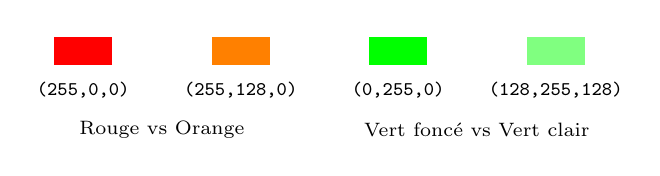
\begin{tikzpicture}
% Rouge vs Orange
\node at (0, 0) {\colorbox[RGB]{255,0,0}{\phantom{aaa}}};
\node at (2, 0) {\colorbox[RGB]{255,128,0}{\phantom{aaa}}};
\node at (0, -0.5) {\scriptsize \texttt{(255,0,0)}};
\node at (2, -0.5) {\scriptsize \texttt{(255,128,0)}};
\node at (1, -1) {\scriptsize Rouge vs Orange};

% Vert foncé vs Vert clair
\node at (4, 0) {\colorbox[RGB]{0,255,0}{\phantom{aaa}}};
\node at (6, 0) {\colorbox[RGB]{128,255,128}{\phantom{aaa}}};
\node at (4, -0.5) {\scriptsize \texttt{(0,255,0)}};
\node at (6, -0.5) {\scriptsize \texttt{(128,255,128)}};
\node at (5, -1) {\scriptsize Vert foncé vs Vert clair};
\end{tikzpicture}
\end{minipage}

\vspace{0.8em}
\hspace{1em}• \textit{→ RGB ne reflète pas toujours la perception humaine}

\pause
\vspace{0.5em}
\textbf{3. BRIEF Lab} \\
\hspace{1em}• Comparaison dans l’espace Lab : \\
\hspace{2em}– $L$ : luminosité (luminance) \\
\hspace{2em}– $a$, $b$ : composantes de couleur perceptuelles \\

\end{frame}
\begin{frame}{Comparaison de descripteurs BRIEF : distance de Hamming}
\centering
\small
\note{Plus la distance est faible, plus les points sont similaires.}

\textbf{Descripteur 1 (image gauche)}\\[0.2em]
\texttt{1 \quad 0 \quad 1 \quad 0 \quad 1}
\pause

\vspace{0.8em}
\textbf{Descripteur 2 (image droite)}\\[0.2em]
\texttt{1 \quad 1 \quad 0 \quad 0 \quad 1}
\pause

\vspace{1em}
\textbf{Comparaison bit à bit :}\\[0.5em]
\begin{tabular}{c}
\begin{tabular}{c c c c c}
\textbf{Bit 1} & \textbf{Bit 2} & \textbf{Bit 3} & \textbf{Bit 4} & \textbf{Bit 5} \\
1 & 0 & 1 & 0 & 1 \\
1 & 1 & 0 & 0 & 1 \\
\hline
\textcolor{green}{0} & \textcolor{red}{1} & \textcolor{red}{1} & \textcolor{green}{0} & \textcolor{green}{0}
\end{tabular}
\end{tabular}
\pause

\vspace{1em}
\textbf{Distance de Hamming = nombre de bits différents = } \texttt{2}

\end{frame}


%===========================
\subsection{Algorithme}
%===========================

\begin{frame}[fragile]{Pseudo-code : Appariement de points}
  \scriptsize
\begin{algorithm}[H]
\DontPrintSemicolon
\Input{Points $P_1$ sur image 1, Points $P_2$ sur image 2, Matrice fondamentale $F$}
\Output{Liste de correspondances fiables}

\only<1->{
\BlankLine
\textbf{Pré-tri des points sur image 1} \;
\ForEach{$p \in P_1$}{
    \Si{$p$ n'est pas un coin}{
        retirer $p$ \tcp*{suppression non maximale locale}
    }
}
}

\only<2->{
\BlankLine
\textbf{Filtrage épipolaire} \;
\ForEach{$p_1 \in P_1$}{
    $l \gets F \cdot p_1$ \tcp*{droite épipolaire dans image 2}
    $C(p_1) \gets \{p_2 \in P_2 \mid \text{distance}(p_2, l) < \varepsilon\}$ \;
}
}

\only<3->{
\BlankLine
\textbf{Comparaison des descripteurs BRIEF} \;
\ForEach{$p_1 \in P_1$}{
    $d_1 \gets \text{BRIEF}(p_1)$ \;
    \ForEach{$p_2 \in C(p_1)$}{
        $d_2 \gets \text{BRIEF}(p_2)$ \;
        $h \gets \text{distance\_Hamming}(d_1, d_2)$ \;
        enregistrer $(p_1, p_2, h)$ \;
    }
}
}

\only<4->{
\Return{paires $(p_1, p_2)$ avec plus petite distance de Hamming}
}
\caption{Appariement}
\end{algorithm}

\end{frame}

%===========================
\subsection{Resultat}
%===========================

\begin{frame}{Résultats appariement}
\begin{center}
\includegraphics[width=\linewidth]{capture/app_complet_2.jpeg}\\
\hyperlink{brief-appendix}{
\beamerbutton{Seuil brief}
}
\hyperlink{sift-appendix}{
\beamerbutton{Comparaison avec Sift}
}
\end{center}

\end{frame}

%%%%%%%%%%%%%%%%%%%%%%%%%%%%%%%%%%%%%%%%%%%%%%%%%
\section[Reconstruction]{Reconstruction}
%------------------------------------------------
%++++++++++++++++++++++++++++++++++++++++++++++++
\subsection{Modélisation théorique}
%++++++++++++++++++++++++++++++++++++++++++++++++

\begin{frame}
\frametitle{Les différents repères}

\begin{minipage}{0.48\textwidth}
    \centering
    \includegraphics[width=\linewidth]{capture/cube_tikz.pdf}
    \vspace{0.5em}
    
    {\footnotesize\textbf{Représentation du cube (vue 3D)}}
\end{minipage}
\hfill
\begin{minipage}{0.48\textwidth}
    \centering
    \includegraphics[width=\linewidth]{capture/cube_repere.png}
    \vspace{0.5em}

    {\footnotesize\textbf{Cube sur une image}}
\end{minipage}

\end{frame}


\begin{frame}
\frametitle{Les différents repères}

\begin{minipage}[c]{0.48\linewidth}
  \centering
  \begin{overlayarea}{0.9\linewidth}{4cm}
    \hspace*{-1cm}
    \begin{tikzpicture}[x=0.75pt,y=0.75pt,yscale=-1,xscale=1, scale=0.6]
    \only<1>{


\tikzset{every picture/.style={line width=0.75pt}} %set default line width to 0.75pt        

\begin{tikzpicture}[x=0.75pt,y=0.75pt,yscale=-1,xscale=1]
%uncomment if require: \path (0,300); %set diagram left start at 0, and has height of 300

%Shape: Rectangle [id:dp9723727103024109] 
\draw  [line width=0.75]  (273.11,2.68) -- (273.16,155.68) -- (150.53,258.66) -- (150.47,105.66) -- cycle ;
%Shape: Circle [id:dp9239162914529644] 
\draw   (170.87,132.32) .. controls (172.23,131.96) and (173.33,132.77) .. (173.33,134.13) .. controls (173.33,135.49) and (172.23,136.89) .. (170.87,137.26) .. controls (169.5,137.62) and (168.4,136.81) .. (168.4,135.45) .. controls (168.4,134.09) and (169.5,132.69) .. (170.87,132.32) -- cycle ;
%Straight Lines [id:da4507743094695521] 
\draw  [dash pattern={on 0.84pt off 2.51pt}]  (211.82,130.67) -- (45,134.7) ;
%Shape: Circle [id:dp9335082203579057] 
\draw   (499.62,131.92) .. controls (500.98,131.55) and (502.08,132.36) .. (502.08,133.72) .. controls (502.08,135.09) and (500.98,136.49) .. (499.62,136.85) .. controls (498.25,137.22) and (497.15,136.41) .. (497.15,135.05) .. controls (497.15,133.68) and (498.25,132.28) .. (499.62,131.92) -- cycle ;
%Shape: Circle [id:dp5162114026007054] 
\draw  [color={rgb, 255:red, 241; green, 53; blue, 53 }  ,draw opacity=1 ] (512.82,105.92) .. controls (514.18,105.55) and (515.28,106.36) .. (515.28,107.72) .. controls (515.28,109.09) and (514.18,110.49) .. (512.82,110.85) .. controls (511.45,111.22) and (510.35,110.41) .. (510.35,109.05) .. controls (510.35,107.68) and (511.45,106.28) .. (512.82,105.92) -- cycle ;
%Shape: Circle [id:dp4319786220460511] 
\draw  [fill={rgb, 255:red, 0; green, 0; blue, 0 }  ,fill opacity=1 ] (321.12,132.42) .. controls (322.48,132.42) and (323.58,133.52) .. (323.58,134.88) .. controls (323.58,136.25) and (322.48,137.35) .. (321.12,137.35) .. controls (319.75,137.35) and (318.65,136.25) .. (318.65,134.88) .. controls (318.65,133.52) and (319.75,132.42) .. (321.12,132.42) -- cycle ;
%Straight Lines [id:da5164589906920809] 
\draw    (321.12,134.88) -- (321.97,70.75) ;
\draw [shift={(322,68.75)}, rotate = 90.77] [color={rgb, 255:red, 0; green, 0; blue, 0 }  ][line width=0.75]    (10.93,-3.29) .. controls (6.95,-1.4) and (3.31,-0.3) .. (0,0) .. controls (3.31,0.3) and (6.95,1.4) .. (10.93,3.29)   ;
%Straight Lines [id:da7854412907443913] 
\draw    (321.12,134.88) -- (253.5,134.75) ;
\draw [shift={(251.5,134.75)}, rotate = 0.11] [color={rgb, 255:red, 0; green, 0; blue, 0 }  ][line width=0.75]    (10.93,-3.29) .. controls (6.95,-1.4) and (3.31,-0.3) .. (0,0) .. controls (3.31,0.3) and (6.95,1.4) .. (10.93,3.29)   ;
%Straight Lines [id:da3058610918194634] 
\draw    (321.12,134.88) -- (272.48,176.16) ;
\draw [shift={(270.95,177.45)}, rotate = 319.68] [color={rgb, 255:red, 0; green, 0; blue, 0 }  ][line width=0.75]    (10.93,-3.29) .. controls (6.95,-1.4) and (3.31,-0.3) .. (0,0) .. controls (3.31,0.3) and (6.95,1.4) .. (10.93,3.29)   ;
%Straight Lines [id:da5453100201962917] 
\draw  [dash pattern={on 4.5pt off 4.5pt}]  (149.63,172.62) -- (150.47,105.66) ;
\draw [shift={(149.61,174.62)}, rotate = 270.72] [color={rgb, 255:red, 0; green, 0; blue, 0 }  ][line width=0.75]    (10.93,-3.29) .. controls (6.95,-1.4) and (3.31,-0.3) .. (0,0) .. controls (3.31,0.3) and (6.95,1.4) .. (10.93,3.29)   ;
%Straight Lines [id:da4691798453437107] 
\draw  [dash pattern={on 4.5pt off 4.5pt}]  (199.11,64.39) -- (150.47,105.66) ;
\draw [shift={(200.64,63.1)}, rotate = 139.68] [color={rgb, 255:red, 0; green, 0; blue, 0 }  ][line width=0.75]    (10.93,-3.29) .. controls (6.95,-1.4) and (3.31,-0.3) .. (0,0) .. controls (3.31,0.3) and (6.95,1.4) .. (10.93,3.29)   ;
%Straight Lines [id:da9224741393814412] 
\draw [color={rgb, 255:red, 241; green, 45; blue, 45 }  ,draw opacity=1 ]   (512.82,108.38) -- (192.48,152.97) ;
\draw [shift={(190.5,153.25)}, rotate = 352.08] [color={rgb, 255:red, 241; green, 45; blue, 45 }  ,draw opacity=1 ][line width=0.75]    (10.93,-3.29) .. controls (6.95,-1.4) and (3.31,-0.3) .. (0,0) .. controls (3.31,0.3) and (6.95,1.4) .. (10.93,3.29)   ;
%Shape: Circle [id:dp7585208638434278] 
\draw  [color={rgb, 255:red, 241; green, 53; blue, 53 }  ,draw opacity=1 ] (190.5,150.78) .. controls (191.86,150.42) and (192.97,151.23) .. (192.97,152.59) .. controls (192.97,153.95) and (191.86,155.35) .. (190.5,155.72) .. controls (189.14,156.08) and (188.03,155.27) .. (188.03,153.91) .. controls (188.03,152.55) and (189.14,151.15) .. (190.5,150.78) -- cycle ;
%Shape: Cube [id:dp7714367112041981] 
\draw   (499.62,131.92) -- (520.32,111.22) -- (568.62,111.22) -- (568.62,160.52) -- (547.92,181.22) -- (499.62,181.22) -- cycle ; \draw   (568.62,111.22) -- (547.92,131.92) -- (499.62,131.92) ; \draw   (547.92,131.92) -- (547.92,181.22) ;

% Text Node
\draw (517,97.9) node [anchor=north west][inner sep=0.75pt]  [font=\footnotesize,color={rgb, 255:red, 167; green, 17; blue, 17 }  ,opacity=1 ]  {$P$};
% Text Node
\draw (324,59.9) node [anchor=north west][inner sep=0.75pt]  [font=\footnotesize]  {$\vec{j}$};
% Text Node
\draw (280.5,178.9) node [anchor=north west][inner sep=0.75pt]  [font=\footnotesize]  {$\vec{i}$};
% Text Node
\draw (324.43,139.84) node [anchor=north west][inner sep=0.75pt]  [font=\footnotesize]  {$O$};
% Text Node
\draw (252,112.9) node [anchor=north west][inner sep=0.75pt]  [font=\footnotesize]  {$\vec{k}$};
% Text Node
\draw (158.65,118.28) node [anchor=north west][inner sep=0.75pt]  [font=\footnotesize]  {$C$};
% Text Node
\draw (156,62.9) node [anchor=north west][inner sep=0.75pt]  [font=\footnotesize]  {$\vec{u}$};
% Text Node
\draw (125.5,114.4) node [anchor=north west][inner sep=0.75pt]  [font=\footnotesize]  {$\vec{v}$};
% Text Node
\draw (184.5,155.9) node [anchor=north west][inner sep=0.75pt]  [font=\footnotesize,color={rgb, 255:red, 159; green, 16; blue, 16 }  ,opacity=1 ]  {$P'$};


\end{tikzpicture}}
    \only<2>{
%Shape: Rectangle [id:dp4318964674614302] 
\draw  [line width=0.75]  (261.98,12.03) -- (262.02,142.84) -- (150.52,236.47) -- (150.47,105.66) -- cycle ;
%Shape: Circle [id:dp8619322586517022] 
\draw  [color={rgb, 255:red, 16; green, 18; blue, 125 }  ,draw opacity=1 ][fill={rgb, 255:red, 16; green, 18; blue, 125 }  ,fill opacity=1 ] (350.47,93.07) .. controls (351.83,92.71) and (352.93,93.52) .. (352.93,94.88) .. controls (352.93,96.24) and (351.83,97.64) .. (350.47,98.01) .. controls (349.1,98.37) and (348,97.56) .. (348,96.2) .. controls (348,94.84) and (349.1,93.44) .. (350.47,93.07) -- cycle ;
%Shape: Cube [id:dp5712797611314612] 
\draw   (325.13,88.8) -- (342.27,71.67) -- (382.25,71.67) -- (382.25,112.75) -- (365.12,129.88) -- (325.13,129.88) -- cycle ; \draw   (382.25,71.67) -- (365.12,88.8) -- (325.13,88.8) ; \draw   (365.12,88.8) -- (365.12,129.88) ;
%Shape: Rectangle [id:dp6697517945708218] 
\draw  [color={rgb, 255:red, 255; green, 255; blue, 255 }  ,draw opacity=1 ] (41.02,5.34) -- (469,5.34) -- (469,280.34) -- (41.02,280.34) -- cycle ;

% Text Node
\draw (358,50.9) node [anchor=north west][inner sep=0.75pt]  [font=\footnotesize,color={rgb, 255:red, 16; green, 18; blue, 125 }  ,opacity=1 ]  {$M$};}
    \only<3>{\input{donnees/s2_3.tex}}
    \only<4>{\input{donnees/s2_4.tex}}
    \only<5>{
\draw  [line width=0.75]  (261.98,12.03) -- (262.02,142.84) -- (150.52,236.47) -- (150.47,105.66) -- cycle ;
%Shape: Circle [id:dp0391503239902703] 
\draw  [color={rgb, 255:red, 16; green, 18; blue, 125 }  ,draw opacity=1 ][fill={rgb, 255:red, 16; green, 18; blue, 125 }  ,fill opacity=1 ] (350.47,93.07) .. controls (351.83,92.71) and (352.93,93.52) .. (352.93,94.88) .. controls (352.93,96.24) and (351.83,97.64) .. (350.47,98.01) .. controls (349.1,98.37) and (348,97.56) .. (348,96.2) .. controls (348,94.84) and (349.1,93.44) .. (350.47,93.07) -- cycle ;
%Shape: Circle [id:dp8654606077158083] 
\draw  [fill={rgb, 255:red, 0; green, 0; blue, 0 }  ,fill opacity=1 ] (365.12,130.42) .. controls (366.48,130.42) and (367.58,131.52) .. (367.58,132.88) .. controls (367.58,134.25) and (366.48,135.35) .. (365.12,135.35) .. controls (363.75,135.35) and (362.65,134.25) .. (362.65,132.88) .. controls (362.65,131.52) and (363.75,130.42) .. (365.12,130.42) -- cycle ;
%Straight Lines [id:da3675337375445349] 
\draw  [dash pattern={on 4.5pt off 4.5pt}]  (150.02,143.52) -- (150.47,105.66) ;
\draw [shift={(150,145.52)}, rotate = 270.68] [color={rgb, 255:red, 0; green, 0; blue, 0 }  ][line width=0.75]    (10.93,-3.29) .. controls (6.95,-1.4) and (3.31,-0.3) .. (0,0) .. controls (3.31,0.3) and (6.95,1.4) .. (10.93,3.29)   ;
%Straight Lines [id:da2135082456633841] 
\draw  [dash pattern={on 4.5pt off 4.5pt}]  (182.47,78.8) -- (150.47,105.66) ;
\draw [shift={(184,77.52)}, rotate = 139.99] [color={rgb, 255:red, 0; green, 0; blue, 0 }  ][line width=0.75]    (10.93,-3.29) .. controls (6.95,-1.4) and (3.31,-0.3) .. (0,0) .. controls (3.31,0.3) and (6.95,1.4) .. (10.93,3.29)   ;
%Shape: Circle [id:dp3919067214179274] 
\draw  [color={rgb, 255:red, 16; green, 18; blue, 125 }  ,draw opacity=1 ] (209.53,118.71) .. controls (210.9,118.35) and (212,119.15) .. (212,120.52) .. controls (212,121.88) and (210.9,123.28) .. (209.53,123.64) .. controls (208.17,124.01) and (207.07,123.2) .. (207.07,121.84) .. controls (207.07,120.48) and (208.17,119.08) .. (209.53,118.71) -- cycle ;
%Straight Lines [id:da13961882146045834] 
\draw [color={rgb, 255:red, 16; green, 18; blue, 125 }  ,draw opacity=1 ][fill={rgb, 255:red, 16; green, 18; blue, 125 }  ,fill opacity=1 ]   (350.47,95.54) -- (212,120.52) ;
%Straight Lines [id:da6009765896576962] 
\draw    (365.12,130.42) -- (331,129.27) ;
\draw [shift={(329,129.2)}, rotate = 1.93] [color={rgb, 255:red, 0; green, 0; blue, 0 }  ][line width=0.75]    (10.93,-3.29) .. controls (6.95,-1.4) and (3.31,-0.3) .. (0,0) .. controls (3.31,0.3) and (6.95,1.4) .. (10.93,3.29)   ;
%Straight Lines [id:da13460515919081129] 
\draw    (365.12,130.42) -- (380.86,114.19) ;
\draw [shift={(382.25,112.75)}, rotate = 134.12] [color={rgb, 255:red, 0; green, 0; blue, 0 }  ][line width=0.75]    (10.93,-3.29) .. controls (6.95,-1.4) and (3.31,-0.3) .. (0,0) .. controls (3.31,0.3) and (6.95,1.4) .. (10.93,3.29)   ;
%Straight Lines [id:da5115010168409273] 
\draw    (364.65,132.88) -- (364.04,100.2) ;
\draw [shift={(364,98.2)}, rotate = 88.93] [color={rgb, 255:red, 0; green, 0; blue, 0 }  ][line width=0.75]    (10.93,-3.29) .. controls (6.95,-1.4) and (3.31,-0.3) .. (0,0) .. controls (3.31,0.3) and (6.95,1.4) .. (10.93,3.29)   ;
%Shape: Cube [id:dp47417096557677685] 
\draw   (325.13,88.8) -- (342.27,71.67) -- (382.25,71.67) -- (382.25,112.75) -- (365.12,129.88) -- (325.13,129.88) -- cycle ; \draw   (382.25,71.67) -- (365.12,88.8) -- (325.13,88.8) ; \draw   (365.12,88.8) -- (365.12,129.88) ;
%Shape: Rectangle [id:dp12317704811349806] 
\draw  [color={rgb, 255:red, 255; green, 255; blue, 255 }  ,draw opacity=1 ] (41.02,5.34) -- (469,5.34) -- (469,280.34) -- (41.02,280.34) -- cycle ;

% Text Node
\draw (358,50.9) node [anchor=north west][inner sep=0.75pt]  [font=\footnotesize,color={rgb, 255:red, 16; green, 18; blue, 125 }  ,opacity=1 ]  {$M$};
% Text Node
\draw (364.65,136.28) node [anchor=north west][inner sep=0.75pt]  [font=\footnotesize]  {$W$};
% Text Node
\draw (154,71.9) node [anchor=north west][inner sep=0.75pt]  [font=\footnotesize]  {$u'$};
% Text Node
\draw (129.5,109.4) node [anchor=north west][inner sep=0.75pt]  [font=\footnotesize]  {$v'$};
% Text Node
\draw (210,99.9) node [anchor=north west][inner sep=0.75pt]  [font=\footnotesize,color={rgb, 255:red, 167; green, 17; blue, 17 }  ,opacity=1 ]  {$\textcolor[rgb]{0.06,0.07,0.49}{m}$};
}
    \only<6>{
%Shape: Rectangle [id:dp22091086801975413] 
\draw  [line width=0.75]  (261.98,12.03) -- (262.02,142.84) -- (150.52,236.47) -- (150.47,105.66) -- cycle ;
%Shape: Circle [id:dp3960031807548443] 
\draw  [color={rgb, 255:red, 16; green, 18; blue, 125 }  ,draw opacity=1 ][fill={rgb, 255:red, 16; green, 18; blue, 125 }  ,fill opacity=1 ] (350.47,93.07) .. controls (351.83,92.71) and (352.93,93.52) .. (352.93,94.88) .. controls (352.93,96.24) and (351.83,97.64) .. (350.47,98.01) .. controls (349.1,98.37) and (348,97.56) .. (348,96.2) .. controls (348,94.84) and (349.1,93.44) .. (350.47,93.07) -- cycle ;
%Shape: Circle [id:dp7170017338469822] 
\draw  [fill={rgb, 255:red, 0; green, 0; blue, 0 }  ,fill opacity=1 ] (365.12,130.42) .. controls (366.48,130.42) and (367.58,131.52) .. (367.58,132.88) .. controls (367.58,134.25) and (366.48,135.35) .. (365.12,135.35) .. controls (363.75,135.35) and (362.65,134.25) .. (362.65,132.88) .. controls (362.65,131.52) and (363.75,130.42) .. (365.12,130.42) -- cycle ;
%Straight Lines [id:da925005109202037] 
\draw  [dash pattern={on 4.5pt off 4.5pt}]  (150.02,143.52) -- (150.47,105.66) ;
\draw [shift={(150,145.52)}, rotate = 270.68] [color={rgb, 255:red, 0; green, 0; blue, 0 }  ][line width=0.75]    (10.93,-3.29) .. controls (6.95,-1.4) and (3.31,-0.3) .. (0,0) .. controls (3.31,0.3) and (6.95,1.4) .. (10.93,3.29)   ;
%Straight Lines [id:da7341104591578826] 
\draw  [dash pattern={on 4.5pt off 4.5pt}]  (182.47,78.8) -- (150.47,105.66) ;
\draw [shift={(184,77.52)}, rotate = 139.99] [color={rgb, 255:red, 0; green, 0; blue, 0 }  ][line width=0.75]    (10.93,-3.29) .. controls (6.95,-1.4) and (3.31,-0.3) .. (0,0) .. controls (3.31,0.3) and (6.95,1.4) .. (10.93,3.29)   ;
%Shape: Circle [id:dp054443755291766927] 
\draw  [color={rgb, 255:red, 16; green, 18; blue, 125 }  ,draw opacity=1 ] (209.53,118.71) .. controls (210.9,118.35) and (212,119.15) .. (212,120.52) .. controls (212,121.88) and (210.9,123.28) .. (209.53,123.64) .. controls (208.17,124.01) and (207.07,123.2) .. (207.07,121.84) .. controls (207.07,120.48) and (208.17,119.08) .. (209.53,118.71) -- cycle ;
%Straight Lines [id:da5500031803707174] 
\draw [color={rgb, 255:red, 16; green, 18; blue, 125 }  ,draw opacity=1 ][fill={rgb, 255:red, 16; green, 18; blue, 125 }  ,fill opacity=1 ]   (350.47,95.54) -- (212,120.52) ;
%Straight Lines [id:da19418058541638872] 
\draw    (365.12,130.42) -- (331,129.27) ;
\draw [shift={(329,129.2)}, rotate = 1.93] [color={rgb, 255:red, 0; green, 0; blue, 0 }  ][line width=0.75]    (10.93,-3.29) .. controls (6.95,-1.4) and (3.31,-0.3) .. (0,0) .. controls (3.31,0.3) and (6.95,1.4) .. (10.93,3.29)   ;
%Straight Lines [id:da06456179839803622] 
\draw    (365.12,130.42) -- (380.86,114.19) ;
\draw [shift={(382.25,112.75)}, rotate = 134.12] [color={rgb, 255:red, 0; green, 0; blue, 0 }  ][line width=0.75]    (10.93,-3.29) .. controls (6.95,-1.4) and (3.31,-0.3) .. (0,0) .. controls (3.31,0.3) and (6.95,1.4) .. (10.93,3.29)   ;
%Straight Lines [id:da6878817592231475] 
\draw    (364.65,132.88) -- (364.04,100.2) ;
\draw [shift={(364,98.2)}, rotate = 88.93] [color={rgb, 255:red, 0; green, 0; blue, 0 }  ][line width=0.75]    (10.93,-3.29) .. controls (6.95,-1.4) and (3.31,-0.3) .. (0,0) .. controls (3.31,0.3) and (6.95,1.4) .. (10.93,3.29)   ;
%Shape: Cube [id:dp39297068054343187] 
\draw   (325.13,88.8) -- (342.27,71.67) -- (382.25,71.67) -- (382.25,112.75) -- (365.12,129.88) -- (325.13,129.88) -- cycle ; \draw   (382.25,71.67) -- (365.12,88.8) -- (325.13,88.8) ; \draw   (365.12,88.8) -- (365.12,129.88) ;
%Straight Lines [id:da3701505179737167] 
\draw [color={rgb, 255:red, 0; green, 0; blue, 0 }  ,draw opacity=1 ]   (75.12,154.88) -- (75.97,90.75) ;
\draw [shift={(76,88.75)}, rotate = 90.77] [color={rgb, 255:red, 0; green, 0; blue, 0 }  ,draw opacity=1 ][line width=0.75]    (10.93,-3.29) .. controls (6.95,-1.4) and (3.31,-0.3) .. (0,0) .. controls (3.31,0.3) and (6.95,1.4) .. (10.93,3.29)   ;
%Straight Lines [id:da9863793705895071] 
\draw [color={rgb, 255:red, 0; green, 0; blue, 0 }  ,draw opacity=1 ]   (75.12,154.88) -- (116.31,128.59) ;
\draw [shift={(118,127.52)}, rotate = 147.45] [color={rgb, 255:red, 0; green, 0; blue, 0 }  ,draw opacity=1 ][line width=0.75]    (10.93,-3.29) .. controls (6.95,-1.4) and (3.31,-0.3) .. (0,0) .. controls (3.31,0.3) and (6.95,1.4) .. (10.93,3.29)   ;
%Straight Lines [id:da21691112687890424] 
\draw [color={rgb, 255:red, 0; green, 0; blue, 0 }  ,draw opacity=1 ]   (75.12,154.88) -- (128,153.57) ;
\draw [shift={(130,153.52)}, rotate = 178.57] [color={rgb, 255:red, 0; green, 0; blue, 0 }  ,draw opacity=1 ][line width=0.75]    (10.93,-3.29) .. controls (6.95,-1.4) and (3.31,-0.3) .. (0,0) .. controls (3.31,0.3) and (6.95,1.4) .. (10.93,3.29)   ;
%Straight Lines [id:da5973484313893659] 
\draw [color={rgb, 255:red, 16; green, 18; blue, 125 }  ,draw opacity=1 ]   (157,133.52) -- (75.12,154.88) ;
%Straight Lines [id:da9607014603660214] 
\draw [color={rgb, 255:red, 0; green, 0; blue, 0 }  ,draw opacity=1 ] [dash pattern={on 0.84pt off 2.51pt}]  (211.07,120.84) -- (157,133.52) ;
%Shape: Rectangle [id:dp47930549648846155] 
\draw  [color={rgb, 255:red, 255; green, 255; blue, 255 }  ,draw opacity=1 ] (41.02,5.34) -- (469,5.34) -- (469,280.34) -- (41.02,280.34) -- cycle ;

% Text Node
\draw (358,50.9) node [anchor=north west][inner sep=0.75pt]  [font=\footnotesize,color={rgb, 255:red, 16; green, 18; blue, 125 }  ,opacity=1 ]  {$M$};
% Text Node
\draw (364.65,136.28) node [anchor=north west][inner sep=0.75pt]  [font=\footnotesize]  {$W$};
% Text Node
\draw (154,71.9) node [anchor=north west][inner sep=0.75pt]  [font=\footnotesize]  {$u'$};
% Text Node
\draw (129.5,109.4) node [anchor=north west][inner sep=0.75pt]  [font=\footnotesize]  {$v'$};
% Text Node
\draw (210,99.9) node [anchor=north west][inner sep=0.75pt]  [font=\footnotesize,color={rgb, 255:red, 167; green, 17; blue, 17 }  ,opacity=1 ]  {$\textcolor[rgb]{0.06,0.07,0.49}{m}$};
% Text Node
\draw (56.65,159.28) node [anchor=north west][inner sep=0.75pt]  [font=\footnotesize]  {$C$};
% Text Node
\draw (61,70.9) node [anchor=north west][inner sep=0.75pt]  [font=\footnotesize]  {$y$};
}
    \only<7>{\input{donnees/s2_7.tex}}
    \only<8>{
%Shape: Rectangle [id:dp20518050829306933] 
\draw  [line width=0.75]  (261.98,12.03) -- (262.02,142.84) -- (150.52,236.47) -- (150.47,105.66) -- cycle ;
%Shape: Circle [id:dp48036249842364387] 
\draw  [color={rgb, 255:red, 16; green, 18; blue, 125 }  ,draw opacity=1 ][fill={rgb, 255:red, 16; green, 18; blue, 125 }  ,fill opacity=1 ] (350.47,93.07) .. controls (351.83,92.71) and (352.93,93.52) .. (352.93,94.88) .. controls (352.93,96.24) and (351.83,97.64) .. (350.47,98.01) .. controls (349.1,98.37) and (348,97.56) .. (348,96.2) .. controls (348,94.84) and (349.1,93.44) .. (350.47,93.07) -- cycle ;
%Shape: Circle [id:dp15975553735025072] 
\draw  [fill={rgb, 255:red, 0; green, 0; blue, 0 }  ,fill opacity=1 ] (365.12,130.42) .. controls (366.48,130.42) and (367.58,131.52) .. (367.58,132.88) .. controls (367.58,134.25) and (366.48,135.35) .. (365.12,135.35) .. controls (363.75,135.35) and (362.65,134.25) .. (362.65,132.88) .. controls (362.65,131.52) and (363.75,130.42) .. (365.12,130.42) -- cycle ;
%Straight Lines [id:da04569264629085701] 
\draw  [dash pattern={on 4.5pt off 4.5pt}]  (150.02,143.52) -- (150.47,105.66) ;
\draw [shift={(150,145.52)}, rotate = 270.68] [color={rgb, 255:red, 0; green, 0; blue, 0 }  ][line width=0.75]    (10.93,-3.29) .. controls (6.95,-1.4) and (3.31,-0.3) .. (0,0) .. controls (3.31,0.3) and (6.95,1.4) .. (10.93,3.29)   ;
%Straight Lines [id:da34135028023903646] 
\draw  [dash pattern={on 4.5pt off 4.5pt}]  (182.47,78.8) -- (150.47,105.66) ;
\draw [shift={(184,77.52)}, rotate = 139.99] [color={rgb, 255:red, 0; green, 0; blue, 0 }  ][line width=0.75]    (10.93,-3.29) .. controls (6.95,-1.4) and (3.31,-0.3) .. (0,0) .. controls (3.31,0.3) and (6.95,1.4) .. (10.93,3.29)   ;
%Shape: Circle [id:dp9804788379329312] 
\draw  [color={rgb, 255:red, 16; green, 18; blue, 125 }  ,draw opacity=1 ] (209.53,118.71) .. controls (210.9,118.35) and (212,119.15) .. (212,120.52) .. controls (212,121.88) and (210.9,123.28) .. (209.53,123.64) .. controls (208.17,124.01) and (207.07,123.2) .. (207.07,121.84) .. controls (207.07,120.48) and (208.17,119.08) .. (209.53,118.71) -- cycle ;
%Straight Lines [id:da9492695065393072] 
\draw [color={rgb, 255:red, 16; green, 18; blue, 125 }  ,draw opacity=1 ][fill={rgb, 255:red, 16; green, 18; blue, 125 }  ,fill opacity=1 ]   (350.47,95.54) -- (212,120.52) ;
%Straight Lines [id:da3349950281049371] 
\draw    (365.12,130.42) -- (331,129.27) ;
\draw [shift={(329,129.2)}, rotate = 1.93] [color={rgb, 255:red, 0; green, 0; blue, 0 }  ][line width=0.75]    (10.93,-3.29) .. controls (6.95,-1.4) and (3.31,-0.3) .. (0,0) .. controls (3.31,0.3) and (6.95,1.4) .. (10.93,3.29)   ;
%Straight Lines [id:da036984224071377914] 
\draw    (365.12,130.42) -- (380.86,114.19) ;
\draw [shift={(382.25,112.75)}, rotate = 134.12] [color={rgb, 255:red, 0; green, 0; blue, 0 }  ][line width=0.75]    (10.93,-3.29) .. controls (6.95,-1.4) and (3.31,-0.3) .. (0,0) .. controls (3.31,0.3) and (6.95,1.4) .. (10.93,3.29)   ;
%Straight Lines [id:da6787819066580656] 
\draw    (364.65,132.88) -- (364.04,100.2) ;
\draw [shift={(364,98.2)}, rotate = 88.93] [color={rgb, 255:red, 0; green, 0; blue, 0 }  ][line width=0.75]    (10.93,-3.29) .. controls (6.95,-1.4) and (3.31,-0.3) .. (0,0) .. controls (3.31,0.3) and (6.95,1.4) .. (10.93,3.29)   ;
%Shape: Cube [id:dp8344554965778904] 
\draw   (325.13,88.8) -- (342.27,71.67) -- (382.25,71.67) -- (382.25,112.75) -- (365.12,129.88) -- (325.13,129.88) -- cycle ; \draw   (382.25,71.67) -- (365.12,88.8) -- (325.13,88.8) ; \draw   (365.12,88.8) -- (365.12,129.88) ;
%Straight Lines [id:da9940442974254676] 
\draw [color={rgb, 255:red, 0; green, 0; blue, 0 }  ,draw opacity=1 ] [dash pattern={on 0.84pt off 2.51pt}]  (338,148.2) -- (75.12,154.88) ;
%Straight Lines [id:da09913909765003492] 
\draw [color={rgb, 255:red, 0; green, 0; blue, 0 }  ,draw opacity=1 ]   (75.12,154.88) -- (75.97,90.75) ;
\draw [shift={(76,88.75)}, rotate = 90.77] [color={rgb, 255:red, 0; green, 0; blue, 0 }  ,draw opacity=1 ][line width=0.75]    (10.93,-3.29) .. controls (6.95,-1.4) and (3.31,-0.3) .. (0,0) .. controls (3.31,0.3) and (6.95,1.4) .. (10.93,3.29)   ;
%Straight Lines [id:da954541250044646] 
\draw [color={rgb, 255:red, 0; green, 0; blue, 0 }  ,draw opacity=1 ]   (75.12,154.88) -- (116.31,128.59) ;
\draw [shift={(118,127.52)}, rotate = 147.45] [color={rgb, 255:red, 0; green, 0; blue, 0 }  ,draw opacity=1 ][line width=0.75]    (10.93,-3.29) .. controls (6.95,-1.4) and (3.31,-0.3) .. (0,0) .. controls (3.31,0.3) and (6.95,1.4) .. (10.93,3.29)   ;
%Straight Lines [id:da8173811873321303] 
\draw [color={rgb, 255:red, 0; green, 0; blue, 0 }  ,draw opacity=1 ]   (75.12,154.88) -- (128,153.57) ;
\draw [shift={(130,153.52)}, rotate = 178.57] [color={rgb, 255:red, 0; green, 0; blue, 0 }  ,draw opacity=1 ][line width=0.75]    (10.93,-3.29) .. controls (6.95,-1.4) and (3.31,-0.3) .. (0,0) .. controls (3.31,0.3) and (6.95,1.4) .. (10.93,3.29)   ;
%Straight Lines [id:da6590312752180065] 
\draw [color={rgb, 255:red, 16; green, 18; blue, 125 }  ,draw opacity=1 ]   (157,133.52) -- (75.12,154.88) ;
%Straight Lines [id:da9534946249718639] 
\draw [color={rgb, 255:red, 0; green, 0; blue, 0 }  ,draw opacity=1 ]   (86,179.5) -- (192,178.53) ;
\draw [shift={(194,178.52)}, rotate = 179.48] [color={rgb, 255:red, 0; green, 0; blue, 0 }  ,draw opacity=1 ][line width=0.75]    (10.93,-3.29) .. controls (6.95,-1.4) and (3.31,-0.3) .. (0,0) .. controls (3.31,0.3) and (6.95,1.4) .. (10.93,3.29)   ;
\draw [shift={(84,179.52)}, rotate = 359.48] [color={rgb, 255:red, 0; green, 0; blue, 0 }  ,draw opacity=1 ][line width=0.75]    (10.93,-3.29) .. controls (6.95,-1.4) and (3.31,-0.3) .. (0,0) .. controls (3.31,0.3) and (6.95,1.4) .. (10.93,3.29)   ;
%Straight Lines [id:da2603521647004613] 
\draw [color={rgb, 255:red, 0; green, 0; blue, 0 }  ,draw opacity=1 ] [dash pattern={on 0.84pt off 2.51pt}]  (211.07,120.84) -- (157,133.52) ;
%Shape: Rectangle [id:dp15198164582240803] 
\draw  [color={rgb, 255:red, 255; green, 255; blue, 255 }  ,draw opacity=1 ] (41.02,5.34) -- (469,5.34) -- (469,280.34) -- (41.02,280.34) -- cycle ;
%Straight Lines [id:da6760200769193868] 
\draw    (202.02,152.01) -- (201.04,102.52) ;
\draw [shift={(201,100.52)}, rotate = 88.86] [color={rgb, 255:red, 0; green, 0; blue, 0 }  ][line width=0.75]    (10.93,-3.29) .. controls (6.95,-1.4) and (3.31,-0.3) .. (0,0) .. controls (3.31,0.3) and (6.95,1.4) .. (10.93,3.29)   ;
%Straight Lines [id:da9313328046524404] 
\draw    (202.56,151.13) -- (235.26,132.51) ;
\draw [shift={(237,131.52)}, rotate = 150.34] [color={rgb, 255:red, 0; green, 0; blue, 0 }  ][line width=0.75]    (10.93,-3.29) .. controls (6.95,-1.4) and (3.31,-0.3) .. (0,0) .. controls (3.31,0.3) and (6.95,1.4) .. (10.93,3.29)   ;

% Text Node
\draw (358,50.9) node [anchor=north west][inner sep=0.75pt]  [font=\footnotesize,color={rgb, 255:red, 16; green, 18; blue, 125 }  ,opacity=1 ]  {$M$};
% Text Node
\draw (364.65,136.28) node [anchor=north west][inner sep=0.75pt]  [font=\footnotesize]  {$W$};
% Text Node
\draw (154,71.9) node [anchor=north west][inner sep=0.75pt]  [font=\footnotesize]  {$u'$};
% Text Node
\draw (129.5,109.4) node [anchor=north west][inner sep=0.75pt]  [font=\footnotesize]  {$v'$};
% Text Node
% Text Node
\draw (210,99.9) node [anchor=north west][inner sep=0.75pt]  [font=\footnotesize,color={rgb, 255:red, 167; green, 17; blue, 17 }  ,opacity=1 ]  {$\textcolor[rgb]{0.06,0.07,0.49}{m}$};
% Text Node
\draw (294,159) node [anchor=north west][inner sep=0.75pt]   [align=left] {axe optique};
% Text Node
\draw (126,192.9) node [anchor=north west][inner sep=0.75pt]  [font=\footnotesize]  {$f$};
% Text Node
\draw (56.65,159.28) node [anchor=north west][inner sep=0.75pt]  [font=\footnotesize]  {$C$};
% Text Node
\draw (61,70.9) node [anchor=north west][inner sep=0.75pt]  [font=\footnotesize]  {$y$};
% Text Node
\draw (101,112.9) node [anchor=north west][inner sep=0.75pt]  [font=\footnotesize]  {$x$};
% Text Node
\draw (184.65,156.6) node [anchor=north west][inner sep=0.75pt]  [font=\footnotesize]  {$C'$};
% Text Node
\draw (241,123.9) node [anchor=north west][inner sep=0.75pt]  [font=\footnotesize]  {$v$};
% Text Node
\draw (197,79.92) node [anchor=north west][inner sep=0.75pt]  [font=\footnotesize]  {$u$};

}
    \end{tikzpicture}
  \end{overlayarea}
\end{minipage}
\hfill
\begin{minipage}[c]{0.48\linewidth}
  \vspace*{\fill}
  \begin{itemize}
    \item<2-> $M$ : point réel
    \item<3-> $W$ : origine du repère du monde
    \item<4-> $(u', v')$ : coordonnées dans le plan image en pixels
    \item<5-> $m$ : projection de $M$ dans le plan image
    \item<6-> $C$ : origine du repère de la caméra
    \item<8-> $C'$ : origine du repère de l'image par projection de C
  \end{itemize}
  \vspace*{\fill}
\end{minipage}
\end{frame}

\begin{frame}{Projection d’un point 3D sur le plan image}
\begin{minipage}[c]{0.48\linewidth}
  \begin{overlayarea}{\linewidth}{5cm}
    \only<1>{
      Par le théorème de Thalès (projection perspective) \\[0.3em]
      $\begin{array}{rcl}
      u &=& f x_c \\
      v &=& f y_c \\
      w &=& z_c
      \end{array}$
    }

    \only<2>{
      Par le théorème de Thalès (projection perspective) \\[0.3em]
      $\begin{array}{rcl}
      u &=& f x_c \\
      v &=& f y_c \\
      w &=& z_c
      \end{array}$
      \\[0.5em]
      $\displaystyle
      \begin{bmatrix}
      u \\ v \\ w
      \end{bmatrix}
      =
      \begin{bmatrix}
      f & 0 & 0 & 0 \\
      0 & f & 0 & 0 \\
      0 & 0 & 1 & 0
      \end{bmatrix}
      \begin{bmatrix}
      x_c \\ y_c \\ z_c \\ 1
      \end{bmatrix}
      $
    }

    \only<3>{
      Le changement de repère s’écrit avec une transformation homogène :\\[0.5em]
      $\displaystyle
      \begin{bmatrix}
      x_c \\ y_c \\ z_c \\ 1
      \end{bmatrix}
      =
      \begin{bmatrix}
      R & T \\
      0 & 1
      \end{bmatrix}
      \begin{bmatrix}
      X_w \\ Y_w \\ Z_w \\ 1
      \end{bmatrix}
      $
  
      Où $R \in \mathbb{R}^{3\times3}$ est une rotation, $T \in \mathbb{R}^3$ une translation.
    }
  \end{overlayarea}
\end{minipage}
\hfill
\begin{minipage}[c]{0.48\linewidth}
  \centering
  \begin{overlayarea}{0.9\linewidth}{4cm}
    \hspace*{-1cm}
    \begin{tikzpicture}[x=0.75pt,y=0.75pt,yscale=-1,xscale=1, scale=0.6]
      \input{donnees/s2_9.tex}
    \end{tikzpicture}
  \end{overlayarea}
\end{minipage}
\end{frame}


\begin{frame}{Projection d’un point 3D sur le plan image}
  \centering
    $\displaystyle
    \begin{bmatrix}
    u \\ v \\ w
    \end{bmatrix}
    =
    \begin{bmatrix}
    f & 0 & 0 & 0 \\
    0 & f & 0 & 0 \\
    0 & 0 & 1 & 0
    \end{bmatrix}
    \begin{bmatrix}
    R & T \\
    0 & 1
    \end{bmatrix}
    \begin{bmatrix}
    X_w \\ Y_w \\ Z_w \\ 1
    \end{bmatrix}
    $
\end{frame}

%-----------------------------------------------
\begin{frame}
\frametitle{Les différents repères}

\[
\lambda_i 
\begin{pmatrix}
u^{(i)} \\
v^{(i)} \\
1
\end{pmatrix}
=
\begin{pmatrix}
p_{11} & p_{12} & p_{13} & p_{14} \\
p_{21} & p_{22} & p_{23} & p_{24} \\
p_{31} & p_{32} & p_{33} & p_{34}
\end{pmatrix}
\begin{pmatrix}
x_C^{(i)} \\
y_C^{(i)} \\
z_C^{(i)} \\
1
\end{pmatrix}
\]
\end{frame}


\begin{frame}{Modèle de projection — Matrice \( P \)}

\begin{itemize}
  \item<1-> On considère un point 3D \( M = (X, Y, Z) \)
  \item<2-> Il se projette sur un point image \( m = (u, v) \)

  \item<3-> On cherche une relation linéaire homogène :
  \[
  \lambda
  \begin{bmatrix}
  u \cr v \cr 1
  \end{bmatrix}
  P
  =
  \begin{bmatrix}
  X \cr Y \cr Z \cr 1
  \end{bmatrix}
  \]

  \item<4-> \( P \) est une matrice \( 3 \times 4 \), avec 12 inconnues
  \item<5-> En développant les lignes :
  \[
  \lambda u = p_{11}X + p_{12}Y + p_{13}Z + p_{14}
  \]
  \[
  \lambda v = p_{21}X + p_{22}Y + p_{23}Z + p_{24}
  \]
  \[
  \lambda   = p_{31}X + p_{32}Y + p_{33}Z + p_{34}
  \]
\end{itemize}
\end{frame}

%------------------------

\begin{frame}{Équations sans \(\lambda\) et système matriciel}

\begin{itemize}
  \item<1-> Pour un point donné, on élimine \( \lambda \) :
  
  \[
  u (p_{31}X + p_{32}Y + p_{33}Z + p_{34}) = p_{11}X + p_{12}Y + p_{13}Z + p_{14}
  \]
  \[
  v (p_{31}X + p_{32}Y + p_{33}Z + p_{34}) = p_{21}X + p_{22}Y + p_{23}Z + p_{24}
  \]

  \vspace{0.5em}
   \item<2-> Cela donne un système homogène ...
   \[
   \scriptsize
   \begin{cases}
0= & p_{11} x_{C} +p_{12} y_{C}  +p_{13} z_{C} +p_{14} -p_{31} u x_{C} -p_{32} u  z_{C}  -p_{33} u  z_{C}  -p_{34} u \\
0= &  p_{21} x_{C}  +p_{22} y_{C}  +p_{23} z_{C}  +p_{24} -p_{31} v  x_{C}  -p_{32} v  z_{C}  -p_{33} v  z_{C}  -p_{34} v 
\end{cases}
   \]
  \item<3-> En faisant cela pour n points on obtient un système ...
\end{itemize}

\end{frame}

\begin{frame}{Équations sans \(\lambda\) et système matriciel}
  
\[
\resizebox{\textwidth}{!}{$
\left(
\begin{array}{cccccccccccc}
    x_{C}^{(1)} & y_{C}^{(1)} & z_{C}^{(1)} & 1 & 0 & 0 & 0 & 0 & -u^{( 1)} x{C}^{(1)} & -u^{( 1)}y{C}^{(1)} & -u^{( 1)}z_{C}^{(1)} & -u^{(1)}\\
0 & 0 & 0 & 0 & x_{C}^{( 1)} & y_{C}^{( 1)} & z_{C}^{( 1)} & 1 & -v^{( 1)} x_{C}^{( 1)} & -v^{( 1)} y_{C}^{( 1)} & -v^{( 1)} z_{C}^{( 1)} & -v^{( 1)}\\
\vdots  & \vdots  & \vdots  & \vdots  & \vdots  & \vdots  & \vdots  & \vdots  & \vdots  & \vdots  & \vdots  & \vdots \\
x_{C}^{( i)} & y_{C}^{( i)} & z_{C}^{( i)} & 1 & 0 & 0 & 0 & 0 & -u^{( i)} x_{C}^{( i)} & -u^{( i)} y_{C}^{( i)} & -u^{( i)} z_{C}^{( i)} & -u^{( i)}\\
0 & 0 & 0 & 0 & x_{C}^{( i)} & y_{C}^{( i)} & z_{C}^{( i)} & 1 & -v^{( i)} x_{C}^{( i)} & -v^{( i)} y_{C}^{( i)} & -v^{( i)} z_{C}^{( i)} & -v^{( i)}\\
\vdots  & \vdots  & \vdots  & \vdots  & \vdots  & \vdots  & \vdots  & \vdots  & \vdots  & \vdots  & \vdots  & \vdots \\
x_{C}^{( 6)} & y_{C}^{( 6)} & z_{C}^{( 6)} & 1 & 0 & 0 & 0 & 0 & -u^{( 6)} x_{C}^{( 6)} & -u^{( 6)} y_{C}^{( 6)} & -u^{( 6)} z_{C}^{( 6)} & -u^{( 6)}\\
0 & 0 & 0 & 0 & x_{C}^{( 6)} & y_{C}^{( 6)} & z_{C}^{( 6)} & 1 & -v^{( 6)} x_{C}^{( 6)} & -v^{( 6)} y_{C}^{( 6)} & -v^{( 6)} z_{C}^{( 6)} & -v^{( 6)}
\end{array}
\right)
\begin{pmatrix}
p_{11}\\
p_{12}\\
p_{13}\\
p_{14}\\
p_{21}\\
p_{22}\\
p_{23}\\
p_{24}\\
p_{31}\\
p_{32}\\
p_{33}\\
p_{34}
\end{pmatrix} =\begin{pmatrix}
0\\
0\\
0\\
0\\
0\\
0\\
0\\
0\\
0\\
0\\
0\\
0
\end{pmatrix}
$}
\]
\end{frame}

\subsection{En pratiques}

\begin{frame}{Shootin photo : importance de la prise de vue}
  \centering
  \begin{minipage}{0.48\linewidth}
    \centering
    \begin{figure}
      \centering
      \includegraphics[width=0.48\linewidth]{capture/dodec0.jpg}%
      \includegraphics[width=0.48\linewidth]{capture/dodec1.jpg} \\
      \includegraphics[width=0.48\linewidth]{capture/dodec2.jpg}%
      \includegraphics[width=0.48\linewidth]{capture/dodec3.jpg}
      {\footnotesize\textbf{Vues initiales}}
    \end{figure}
  \end{minipage}
  \hfill
  \begin{minipage}{0.48\linewidth}
    \centering
    \begin{figure}
      \centering
      \includegraphics[width=0.48\linewidth]{capture/dodecf0.jpg}%
      \includegraphics[width=0.48\linewidth]{capture/dodecf1.jpg} \\
      \includegraphics[width=0.48\linewidth]{capture/dodecf2.jpg}%
      \includegraphics[width=0.48\linewidth]{capture/dodecf3.jpg}
      {\footnotesize\textbf{Vues améliorées}}
    \end{figure}
  \end{minipage}
\end{frame}


\begin{frame}{Calibration}
 \centering
  \begin{minipage}{0.48\linewidth}
    \centering
    \begin{figure}
      \centering
      \includegraphics[width=0.7\linewidth]{capture/cube_calibrage.jpg}%
      \caption{Cube calibrage}
    \end{figure}
  \end{minipage}
  \hfill
  \begin{minipage}{0.48\linewidth}
    \centering
    \begin{figure}
      \centering
      \includegraphics[width=0.8\linewidth]{capture/selection.png}%
      \caption{Selection des points}
    \end{figure}
  \end{minipage}
\end{frame}



%------------------------------------------
\subsection{Résolution système}
%------------------------------------------------

\begin{frame}{Résolution système}
  
\[
\resizebox{\textwidth}{!}{$
\left(
\begin{array}{cccccccccccc}
    x_{C}^{(1)} & y_{C}^{(1)} & z_{C}^{(1)} & 1 & 0 & 0 & 0 & 0 & -u^{( 1)} x{C}^{(1)} & -u^{( 1)}y{C}^{(1)} & -u^{( 1)}z_{C}^{(1)} & -u^{(1)}\\
0 & 0 & 0 & 0 & x_{C}^{( 1)} & y_{C}^{( 1)} & z_{C}^{( 1)} & 1 & -v^{( 1)} x_{C}^{( 1)} & -v^{( 1)} y_{C}^{( 1)} & -v^{( 1)} z_{C}^{( 1)} & -v^{( 1)}\\
\vdots  & \vdots  & \vdots  & \vdots  & \vdots  & \vdots  & \vdots  & \vdots  & \vdots  & \vdots  & \vdots  & \vdots \\
x_{C}^{( i)} & y_{C}^{( i)} & z_{C}^{( i)} & 1 & 0 & 0 & 0 & 0 & -u^{( i)} x_{C}^{( i)} & -u^{( i)} y_{C}^{( i)} & -u^{( i)} z_{C}^{( i)} & -u^{( i)}\\
0 & 0 & 0 & 0 & x_{C}^{( i)} & y_{C}^{( i)} & z_{C}^{( i)} & 1 & -v^{( i)} x_{C}^{( i)} & -v^{( i)} y_{C}^{( i)} & -v^{( i)} z_{C}^{( i)} & -v^{( i)}\\
\vdots  & \vdots  & \vdots  & \vdots  & \vdots  & \vdots  & \vdots  & \vdots  & \vdots  & \vdots  & \vdots  & \vdots \\
x_{C}^{( 6)} & y_{C}^{( 6)} & z_{C}^{( 6)} & 1 & 0 & 0 & 0 & 0 & -u^{( 6)} x_{C}^{( 6)} & -u^{( 6)} y_{C}^{( 6)} & -u^{( 6)} z_{C}^{( 6)} & -u^{( 6)}\\
0 & 0 & 0 & 0 & x_{C}^{( 6)} & y_{C}^{( 6)} & z_{C}^{( 6)} & 1 & -v^{( 6)} x_{C}^{( 6)} & -v^{( 6)} y_{C}^{( 6)} & -v^{( 6)} z_{C}^{( 6)} & -v^{( 6)}
\end{array}
\right)
\begin{pmatrix}
p_{11}\\
p_{12}\\
p_{13}\\
p_{14}\\
p_{21}\\
p_{22}\\
p_{23}\\
p_{24}\\
p_{31}\\
p_{32}\\
p_{33}\\
p_{34}
\end{pmatrix} =\begin{pmatrix}
0\\
0\\
0\\
0\\
0\\
0\\
0\\
0\\
0\\
0\\
0\\
0
\end{pmatrix}
$}
\]
\end{frame}

\begin{frame}{Problème d’optimisation sous contrainte}
\note{
Résolution classique -> solution triviale nulle 
Le système est homogène -> on peut fixé la norme du vecteur $p$ à 1.
On transforme le problème en une minimisation sous contrainte.

En appliquant les multiplicateurs de Lagrange, on obtient une condition d’optimalité : le gradient de la fonction est proportionnel au gradient de la contrainte, ce qui donne une équation aux valeurs propres.
}
Solution triviale \( P = 0 \).  
On impose : \( \|p\|^2 = 1 \)

\vspace{0.8em}
On reformule le problème comme une minimisation sous contrainte :
\[
\min_{\|p\| = 1} \|Ap\|^2
\quad \Leftrightarrow \quad
\min_{\|p\| = 1} p^T A^T A p
\]
\pause
\textbf{Propriété clé :} au minimum, \( p \) vérifie :
\[
\boxed{A^T A p = \lambda p}
\]
  \hyperlink{optimisation-appendix}{
    \beamerbutton{Compléments calcul}
  }
\vspace{1em}
\pause
\[
\boxed{\min \|Ap\| \Rightarrow p = \text{un v.p. associé à la plus petite va.p. de } A^T A}
\]

\end{frame}

\begin{frame}{Décomposition en valeurs singulières (SVD)}
\begin{itemize}
  \item On factorise \( A \) : 
  \[
  A = U \Sigma V^T
  \]
  \pause
  \item \( U \) : matrice orthogonale de \( \mathbb{R}^{m \times m} \)
  \pause
  \item \( \Sigma \) : matrice diagonale \( \mathbb{R}^{m \times n} \) contenant les valeurs singulières \( \sigma_1 \geq \sigma_2 \geq \dots \geq \sigma_n \geq 0 \)
  \pause
  \item \( V \) : matrice orthogonale de \( \mathbb{R}^{n \times n} \), ses colonnes sont les vecteurs propres de \( A^T A \), tels que :
  \[
  A^T A v_i = \sigma_i^2 v_i
  \]
\end{itemize}

\note{
La décomposition en valeurs singulières, ou SVD, permet de factoriser n’importe quelle matrice \( A \) en trois matrices : deux orthogonales \( U \) et \( V \), et une diagonale \( \Sigma \) contenant les valeurs singulières.

Ces valeurs sont les racines carrées des valeurs propres de \( A^T A \), classées par ordre décroissant.

\( U \) contient les vecteurs propres de \( AA^T \), \( V \) ceux de \( A^T A \). Autrement dit, chaque colonne \( v_i \) de \( V \) vérifie : \( A^T A v_i = \sigma_i^2 v_i \).

La dernière colonne de \( V \), associée à la plus petite valeur singulière, donne donc directement le vecteur \( p \) recherché.

C’est une méthode très stable numériquement.
}
\end{frame}


%++++++++++++++++++++++++++++++++++++++++++++++++
\subsection{Implémentation}

\begin{frame}{Algorithme QR : principe de convergence}
\scriptsize
\begin{minipage}[t][0.8\textheight][t]{\textwidth}
\vspace*{\fill}
\textbf{Décomposition QR pour l’itération :}
\begin{itemize}
  \item Si \( A = QR \), avec :
  \begin{itemize}
    \scriptsize
    \item \( Q \) une matrice orthogonale (\( Q^T Q = I \)),
    \item \( R \) une matrice triangulaire supérieure,
  \end{itemize}
  \pause
  alors on définit :
  \[
    A' = RQ
  \]
  \pause
  \vspace{-1em}
  \item \( A' \) est \textbf{semblable} à \( A \), car :
  \[
    Q^T A Q = Q^T Q R Q = R Q = A'
  \]
\end{itemize}
\pause
\vspace{-0.3em}
\textbf{Construction de la suite :}
\[
\begin{cases}
A_0 = A \\
\text{À chaque itération : } A_k = Q_k R_k \\
A_{k+1} = R_k Q_k
\end{cases}
\]
\vspace{-0.3em}
\pause
\begin{itemize}
  \item Cette suite \( (A_k) \) converge vers une matrice triangulaire.
  \item Les valeurs propres de \( A_k \) sont identiques à celles de \( A \).
\end{itemize}

\vspace*{\fill}
\end{minipage}

\end{frame}


\begin{frame}{Résolution avec SVD}
\hyperlink{SVD-appendix}{\beamerbutton{Pseudo-code détaillé}}
\begin{itemize}
  \item Produit symétrique : \( A^T A \in \mathbb{R}^{n \times n} \)
  \pause
  \item Décomposition QR : 
  \[
    A^TA = Q_{k-1} \cdots Q_0 \, A_k \, Q_0^T \cdots Q_{k-1}^T
  \]
  \pause
  \item Matrice des vecteurs propres : 
  \[
    V = Q_0 Q_1 \cdots Q_{k-1}
  \]
  \pause
  \item Extraction du vecteur propre associé à la plus petite valeur propre non nulle :
  \[
    v_{i_0} \in V
  \]
\end{itemize}

\end{frame}

\section{Reconstruction des points}
\begin{frame}{Reconstruction : retrouver les coordonnées 3D}
  \vspace*{\fill}
  \begin{itemize}
    \item<1-> On connaît les matrices de projection \( P_1 \) et \( P_2 \)
    \item<2-> Deux points image correspondants :
    \vspace*{-0.5em}
    \[
      m_1 = (u_1, v_1),\quad m_2 = (u_2, v_2)
    \]
    \item<3-> Point 3D inconnu :  \( M= (X , Y, Z) \)
    \item<4-> On a :
    \vspace*{-0.5em}
    \[
      \lambda_1 m_1 = P_1 M,\quad \lambda_2 m_2 = P_2 M
    \]
    \item<5-> Système de 6 équations linéaires homogènes
    \item<6-> Résolution par SVD
  \end{itemize}
  \vspace*{\fill}
\end{frame}



\begin{frame}{Reconstruction 3D multi-vues}
  \begin{minipage}{0.6\linewidth}
    \includegraphics[width=\linewidth]{capture/cloud.png}
    \captionof*{figure}{Nuage de points}
  \end{minipage}
  \hfill
  \begin{minipage}{0.3\linewidth}
    \begin{minipage}{0.4\linewidth}
\fcolorbox{red}{white}{\includegraphics[width=\linewidth]{capture/dodecf1.jpg}}\\[0.5em]
      \fcolorbox{green!50!black}{white}{\includegraphics[width=\linewidth]{capture/dodecf3.jpg}}\\[0.5em]
      \fcolorbox{blue!50!black}{white}{\includegraphics[width=\linewidth]{capture/dodecf5.jpg}}\\[0.5em]
      \fcolorbox{cyan}{white}{\includegraphics[width=\linewidth]{capture/dodecf7.jpg}}
    \end{minipage}
    \hfill
    \begin{minipage}{0.4\linewidth}
      \fcolorbox{red}{white}{\includegraphics[width=\linewidth]{capture/dodecf0.jpg}}\\[0.5em]
      \fcolorbox{green!50!black}{white}{\includegraphics[width=\linewidth]{capture/dodecf2.jpg}}\\[0.5em]
      \fcolorbox{blue!50!black}{white}{\includegraphics[width=\linewidth]{capture/dodecf4.jpg}}\\[0.5em]
      \fcolorbox{cyan}{white}{\includegraphics[width=\linewidth]{capture/dodecf6.jpg}}
    \end{minipage}
  \end{minipage}
\end{frame}
%%%%%%%%%%%%%%%%%%%%%%%%%%%%%%%%%%%%%%%%%%%%%%%%%
\section[Enveloppe Convexe]{Enveloppe Convexe}
%------------------------------------------------
%++++++++++++++++++++++++++++++++++++++++++++++++
%++++++++++++++++++++++++++++++++++++++++++++++++
%------------------------------------------------

\captionsetup[figure]{labelformat=empty}
\tikzset{every picture/.style={line width=0.75pt}} %set default line width to 0.75pt
\begin{frame}{Triangulation}

\begin{center}
\hspace{0.05\textwidth}
\begin{minipage}{0.45\textwidth}
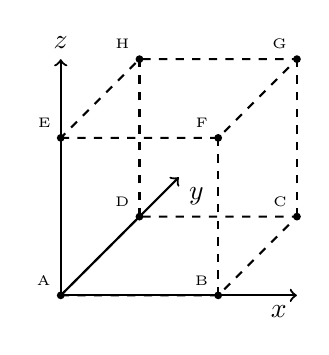
\begin{tikzpicture}[scale=1, x={(1cm,0cm)}, y={(0.5cm,0.5cm)}, z={(0cm,1cm)}]
  % Axes
  \draw[->, thick] (0,0,0) -- (3,0,0) node[anchor=north east] {\(x\)};
  \draw[->, thick] (0,0,0) -- (0,3,0) node[anchor=north west] {\(y\)};
  \draw[->, thick] (0,0,0) -- (0,0,3) node[anchor=south] {\(z\)};

  % Sommets
  \foreach \x/\y/\z/\name in {
    0/0/0/A, 2/0/0/B, 2/2/0/C, 0/2/0/D,
    0/0/2/E, 2/0/2/F, 2/2/2/G, 0/2/2/H}
    {
      \filldraw[black] (\x,\y,\z) circle (1pt) node[anchor=south east] {\tiny \name};
    }

  % Arêtes
  \draw[dashed] (0,0,0) -- (2,0,0) -- (2,2,0) -- (0,2,0) -- cycle;
  \draw[dashed] (0,0,2) -- (2,0,2) -- (2,2,2) -- (0,2,2) -- cycle;
  \draw[dashed] (0,0,0) -- (0,0,2);
  \draw[dashed] (2,0,0) -- (2,0,2);
  \draw[dashed] (2,2,0) -- (2,2,2);
  \draw[dashed] (0,2,0) -- (0,2,2);
\end{tikzpicture}
\end{minipage}
\begin{minipage}{0.45\textwidth}

\begin{tikzpicture}[scale=1, line join=round]
  % Points du cube
  \coordinate (A) at (0,0,0);
  \coordinate (B) at (2,0,0);
  \coordinate (C) at (2,2,0);
  \coordinate (D) at (0,2,0);
  \coordinate (E) at (0,0,2);
  \coordinate (F) at (2,0,2);
  \coordinate (G) at (2,2,2);
  \coordinate (H) at (0,2,2);

  % Triangles - chaque face = 2 triangles
  \fill[blue!50]  (A) -- (B) -- (C) -- cycle;
  \fill[blue!10]  (A) -- (C) -- (D) -- cycle;

  \fill[green!60] (A) -- (B) -- (F) -- cycle;
  \fill[green!20] (A) -- (F) -- (E) -- cycle;

  \fill[red!60]   (B) -- (C) -- (G) -- cycle;
  \fill[red!20]   (B) -- (G) -- (F) -- cycle;

  \fill[yellow!60] (C) -- (D) -- (H) -- cycle;
  \fill[yellow!30] (C) -- (H) -- (G) -- cycle;

 % \fill[orange!50] (D) -- (A) -- (E) -- cycle;
 % \fill[orange!10] (D) -- (E) -- (H) -- cycle;

  \fill[gray!50]   (E) -- (F) -- (G) -- cycle;
  \fill[gray!10]   (E) -- (G) -- (H) -- cycle;

  % Arêtes
%  \draw[thick] (A) -- (B) -- (C) -- (D) -- cycle;
 % \draw[thick] (E) -- (F) -- (G) -- (H) -- cycle;
 % \draw[thick] (A) -- (E);
%  \draw[thick] (B) -- (F);
%  \draw[thick] (C) -- (G);
%  \draw[thick] (D) -- (H);
\end{tikzpicture}
\end{minipage}
\end{center}
\end{frame}

\begin{frame}[fragile]
  \frametitle{Le format \texttt{STL}}

  \begin{columns}
    \column{0.45\textwidth}
    \scriptsize
\begin{verbatim}
solid cube
  facet normal 0 0 1 // Face supérieure
    outer loop
      vertex 0 0 1
      vertex 1 0 1
      vertex 0 1 1
    endloop
  endfacet
  facet normal 0 0 1
    outer loop
      vertex 1 0 1
      vertex 1 1 1
      vertex 0 1 1
    endloop
  endfacet
  // Autres faces...
endsolid cube
\end{verbatim}
    \column{0.55\textwidth}
    \begin{figure}
      \centering
      \includegraphics[width=3.5cm]{capture/cubestl.png} % Remplace par ton image
      \caption{\tiny fichier STL visualisé avec viewstl.com}
    \end{figure}
  \end{columns}
\end{frame}

%%%%%%%%%%%%%%%%%%%%%%%%%%%%%%%%%%%%%%%%%%%%%%%%%
\section[Analyse des résultats]{Analyse des résultats}

%------------------------------------------------
\begin{frame}
\frametitle{Titre d'une slide avant la sous-section}
Ici, on n’a pas encore de titre de sous-section dans le bandeau du haut.\\
\end{frame}


%++++++++++++++++++++++++++++++++++++++++++++++++
\subsection{Quelques exemples}

%------------------------------------------------
\begin{frame}{Aspect pratique}
Ici, on a un titre de sous-section, contrairement à la slide.\\[1.5cm]
Voir le code ici pour référencer une slide avec et la citer avec son numéro via .
\end{frame}

%++++++++++++++++++++++++++++++++++++++++++++++++
\subsection{Critiques}

%------------------------------------------------
\begin{frame}
\frametitle{Titre sans lettre descendant sous la baseline}
Ici c'est mieux, non ?
\end{frame}

\section*[Appendix]{Appendix}
%===============================================
\begin{frame}{Exemple Moravec}
  \label{moravec-appendix}
  \centering
  \begin{tikzpicture}
    \node[anchor=south west,inner sep=0] (image) at (0,0) {\includegraphics[width=0.5\textwidth]{capture/rub_rouge.jpg}};
    \only<2>{\draw[red, thick] (1,4.5) rectangle (2,5.5);}     % rectangle cible
  \end{tikzpicture}
\end{frame}

\begin{frame}
  \note{
    Voici une animation de l’évolution de la détection avec l’algorithme de Moravec.

    On visualise étape par étape comment les coins apparaissent au fur et à mesure.

    Ce genre de visualisation aide à comprendre la sensibilité de l’algorithme selon l’image et les paramètres.
  }
  \centering
  \begin{overlayarea}{0.9\linewidth}{4cm}
    \vspace*{-1cm}
    \hspace*{-1cm}
    \begin{tikzpicture}[x=0.75pt,y=0.75pt,yscale=-1,xscale=1, scale=2]
      \only<1>{
%Shape: Rectangle [id:dp855744465122586] 
\draw  [color={rgb, 255:red, 0; green, 0; blue, 0 }  ,draw opacity=1 ][fill={rgb, 255:red, 200; green, 43; blue, 43 }  ,fill opacity=0.23 ] (279.6,109) -- (299.6,109) -- (299.6,129) -- (279.6,129) -- cycle ;
%Shape: Rectangle [id:dp8201664290630494] 
\draw  [color={rgb, 255:red, 0; green, 0; blue, 0 }  ,draw opacity=1 ][fill={rgb, 255:red, 200; green, 43; blue, 43 }  ,fill opacity=0.64 ] (299.6,129) -- (319.6,129) -- (319.6,149) -- (299.6,149) -- cycle ;
%Shape: Rectangle [id:dp8273756646818722] 
\draw  [color={rgb, 255:red, 0; green, 0; blue, 0 }  ,draw opacity=1 ][fill={rgb, 255:red, 200; green, 43; blue, 43 }  ,fill opacity=0.64 ] (279.6,129) -- (299.6,129) -- (299.6,149) -- (279.6,149) -- cycle ;
%Shape: Rectangle [id:dp6720526871451368] 
\draw  [color={rgb, 255:red, 0; green, 0; blue, 0 }  ,draw opacity=1 ][fill={rgb, 255:red, 200; green, 43; blue, 43 }  ,fill opacity=0.69 ] (299.6,149) -- (319.6,149) -- (319.6,169) -- (299.6,169) -- cycle ;
%Shape: Rectangle [id:dp21990750654974778] 
\draw  [color={rgb, 255:red, 0; green, 0; blue, 0 }  ,draw opacity=1 ][fill={rgb, 255:red, 200; green, 43; blue, 43 }  ,fill opacity=0.68 ] (319.6,129) -- (339.6,129) -- (339.6,149) -- (319.6,149) -- cycle ;
%Shape: Rectangle [id:dp07109720325756996] 
\draw  [color={rgb, 255:red, 0; green, 0; blue, 0 }  ,draw opacity=1 ][fill={rgb, 255:red, 200; green, 43; blue, 43 }  ,fill opacity=0.32 ] (299.6,89) -- (319.6,89) -- (319.6,109) -- (299.6,109) -- cycle ;
%Shape: Rectangle [id:dp9795028573738183] 
\draw  [color={rgb, 255:red, 0; green, 0; blue, 0 }  ,draw opacity=1 ][fill={rgb, 255:red, 200; green, 43; blue, 43 }  ,fill opacity=0.64 ] (299.6,109) -- (319.6,109) -- (319.6,129) -- (299.6,129) -- cycle ;
%Shape: Rectangle [id:dp5174606270935156] 
\draw  [color={rgb, 255:red, 0; green, 0; blue, 0 }  ,draw opacity=1 ][fill={rgb, 255:red, 200; green, 43; blue, 43 }  ,fill opacity=0.23 ] (239.6,69) -- (259.6,69) -- (259.6,89) -- (239.6,89) -- cycle ;
%Shape: Rectangle [id:dp003251435331488195] 
\draw  [color={rgb, 255:red, 0; green, 0; blue, 0 }  ,draw opacity=1 ][fill={rgb, 255:red, 200; green, 43; blue, 43 }  ,fill opacity=0.21 ] (259.6,89) -- (279.6,89) -- (279.6,109) -- (259.6,109) -- cycle ;
%Shape: Rectangle [id:dp12978711061445025] 
\draw  [color={rgb, 255:red, 0; green, 0; blue, 0 }  ,draw opacity=1 ][fill={rgb, 255:red, 200; green, 43; blue, 43 }  ,fill opacity=0.25 ] (239.6,89) -- (259.6,89) -- (259.6,109) -- (239.6,109) -- cycle ;
%Shape: Rectangle [id:dp11386610015932308] 
\draw  [color={rgb, 255:red, 0; green, 0; blue, 0 }  ,draw opacity=1 ][fill={rgb, 255:red, 200; green, 43; blue, 43 }  ,fill opacity=0.28 ] (239.6,109) -- (259.6,109) -- (259.6,129) -- (239.6,129) -- cycle ;
%Shape: Rectangle [id:dp31730737510449536] 
\draw  [color={rgb, 255:red, 0; green, 0; blue, 0 }  ,draw opacity=1 ][fill={rgb, 255:red, 200; green, 43; blue, 43 }  ,fill opacity=0.66 ] (259.6,129) -- (279.6,129) -- (279.6,149) -- (259.6,149) -- cycle ;
%Shape: Rectangle [id:dp0039535950874963754] 
\draw  [color={rgb, 255:red, 0; green, 0; blue, 0 }  ,draw opacity=1 ][fill={rgb, 255:red, 200; green, 43; blue, 43 }  ,fill opacity=0.77 ] (279.6,149) -- (299.6,149) -- (299.6,169) -- (279.6,169) -- cycle ;
%Shape: Rectangle [id:dp5148350575823291] 
\draw  [color={rgb, 255:red, 0; green, 0; blue, 0 }  ,draw opacity=1 ][fill={rgb, 255:red, 200; green, 43; blue, 43 }  ,fill opacity=0.24 ] (259.6,109) -- (279.6,109) -- (279.6,129) -- (259.6,129) -- cycle ;
%Shape: Rectangle [id:dp36043744827539115] 
\draw  [color={rgb, 255:red, 0; green, 0; blue, 0 }  ,draw opacity=1 ][fill={rgb, 255:red, 200; green, 43; blue, 43 }  ,fill opacity=0.26 ] (259.6,69) -- (279.6,69) -- (279.6,89) -- (259.6,89) -- cycle ;
%Shape: Rectangle [id:dp3332412201524424] 
\draw  [color={rgb, 255:red, 0; green, 0; blue, 0 }  ,draw opacity=1 ][fill={rgb, 255:red, 200; green, 43; blue, 43 }  ,fill opacity=0.22 ] (279.6,89) -- (299.6,89) -- (299.6,109) -- (279.6,109) -- cycle ;
%Shape: Rectangle [id:dp49757845918426946] 
\draw  [color={rgb, 255:red, 0; green, 0; blue, 0 }  ,draw opacity=1 ][fill={rgb, 255:red, 200; green, 43; blue, 43 }  ,fill opacity=0.29 ] (279.6,69) -- (299.6,69) -- (299.6,89) -- (279.6,89) -- cycle ;
%Shape: Rectangle [id:dp1948054383738922] 
\draw  [color={rgb, 255:red, 0; green, 0; blue, 0 }  ,draw opacity=1 ][fill={rgb, 255:red, 200; green, 43; blue, 43 }  ,fill opacity=0.28 ] (299.6,69) -- (319.6,69) -- (319.6,89) -- (299.6,89) -- cycle ;
%Shape: Rectangle [id:dp5908482157161481] 
\draw  [color={rgb, 255:red, 0; green, 0; blue, 0 }  ,draw opacity=1 ][fill={rgb, 255:red, 200; green, 43; blue, 43 }  ,fill opacity=0.65 ] (319.6,109) -- (339.6,109) -- (339.6,129) -- (319.6,129) -- cycle ;
%Shape: Rectangle [id:dp8244027566618196] 
\draw  [color={rgb, 255:red, 0; green, 0; blue, 0 }  ,draw opacity=1 ][fill={rgb, 255:red, 200; green, 43; blue, 43 }  ,fill opacity=0.64 ] (239.6,129) -- (259.6,129) -- (259.6,149) -- (239.6,149) -- cycle ;
%Shape: Rectangle [id:dp29418903051156065] 
\draw  [color={rgb, 255:red, 0; green, 0; blue, 0 }  ,draw opacity=1 ][fill={rgb, 255:red, 200; green, 43; blue, 43 }  ,fill opacity=0.73 ] (239.6,149) -- (259.6,149) -- (259.6,169) -- (239.6,169) -- cycle ;
%Shape: Rectangle [id:dp03059484266780088] 
\draw  [color={rgb, 255:red, 0; green, 0; blue, 0 }  ,draw opacity=1 ][fill={rgb, 255:red, 200; green, 43; blue, 43 }  ,fill opacity=0.74 ] (259.6,149) -- (279.6,149) -- (279.6,169) -- (259.6,169) -- cycle ;
%Shape: Rectangle [id:dp15824841679231605] 
\draw  [color={rgb, 255:red, 0; green, 0; blue, 0 }  ,draw opacity=1 ][fill={rgb, 255:red, 200; green, 43; blue, 43 }  ,fill opacity=0.68 ] (319.6,149) -- (339.6,149) -- (339.6,169) -- (319.6,169) -- cycle ;
%Shape: Rectangle [id:dp5219374564422655] 
\draw  [color={rgb, 255:red, 0; green, 0; blue, 0 }  ,draw opacity=1 ][fill={rgb, 255:red, 200; green, 43; blue, 43 }  ,fill opacity=0.7 ] (319.6,69) -- (339.6,69) -- (339.6,89) -- (319.6,89) -- cycle ;
%Shape: Rectangle [id:dp41832573855226485] 
\draw  [color={rgb, 255:red, 0; green, 0; blue, 0 }  ,draw opacity=1 ][fill={rgb, 255:red, 200; green, 43; blue, 43 }  ,fill opacity=0.63 ] (319.6,89) -- (339.6,89) -- (339.6,109) -- (319.6,109) -- cycle ;
%Shape: Rectangle [id:dp4512036699306804] 
\draw  [color={rgb, 255:red, 255; green, 255; blue, 255 }  ,draw opacity=1 ] (209,54.5) -- (451,54.5) -- (451,190.5) -- (209,190.5) -- cycle ;
%Shape: Rectangle [id:dp30277857918883444] 
\draw  [color={rgb, 255:red, 222; green, 195; blue, 14 }  ,draw opacity=1 ][fill={rgb, 255:red, 192; green, 177; blue, 255 }  ,fill opacity=0.34 ] (259.6,335) -- (279.6,335) -- (279.6,355) -- (259.6,355) -- cycle ;

% Text Node
\draw (304.8,136) node [anchor=north west][inner sep=0.75pt]  [font=\footnotesize] [align=left] {64};
% Text Node
\draw (324.8,155.2) node [anchor=north west][inner sep=0.75pt]  [font=\footnotesize] [align=left] {69};
% Text Node
\draw (305.2,115.6) node [anchor=north west][inner sep=0.75pt]  [font=\footnotesize] [align=left] {65};
% Text Node
\draw (305.2,95.6) node [anchor=north west][inner sep=0.75pt]  [font=\footnotesize] [align=left] {32};
% Text Node
\draw (285.2,95.6) node [anchor=north west][inner sep=0.75pt]  [font=\footnotesize] [align=left] {22};
% Text Node
\draw (325.2,115.6) node [anchor=north west][inner sep=0.75pt]  [font=\footnotesize] [align=left] {65};
% Text Node
\draw (244.4,76) node [anchor=north west][inner sep=0.75pt]  [font=\footnotesize] [align=left] {23};
% Text Node
\draw (265.2,96) node [anchor=north west][inner sep=0.75pt]  [font=\footnotesize] [align=left] {21};
% Text Node
\draw (244.8,95.6) node [anchor=north west][inner sep=0.75pt]  [font=\footnotesize] [align=left] {25};
% Text Node
\draw (264.8,116.4) node [anchor=north west][inner sep=0.75pt]  [font=\footnotesize] [align=left] {24};
% Text Node
\draw (284.8,135.6) node [anchor=north west][inner sep=0.75pt]  [font=\footnotesize] [align=left] {64};
% Text Node
\draw (304.8,155.2) node [anchor=north west][inner sep=0.75pt]  [font=\footnotesize] [align=left] {69};
% Text Node
\draw (264.4,75.6) node [anchor=north west][inner sep=0.75pt]  [font=\footnotesize] [align=left] {26};
% Text Node
\draw (285.2,75.6) node [anchor=north west][inner sep=0.75pt]  [font=\footnotesize] [align=left] {29};
% Text Node
\draw (304.8,75.2) node [anchor=north west][inner sep=0.75pt]  [font=\footnotesize] [align=left] {28};
% Text Node
\draw (324.8,95.2) node [anchor=north west][inner sep=0.75pt]  [font=\footnotesize] [align=left] {63};
% Text Node
\draw (324.8,76.8) node [anchor=north west][inner sep=0.75pt]  [font=\footnotesize] [align=left] {70};
% Text Node
\draw (244.8,115.6) node [anchor=north west][inner sep=0.75pt]  [font=\footnotesize] [align=left] {28};
% Text Node
\draw (264.8,135.6) node [anchor=north west][inner sep=0.75pt]  [font=\footnotesize] [align=left] {66};
% Text Node
\draw (284.8,155.2) node [anchor=north west][inner sep=0.75pt]  [font=\footnotesize] [align=left] {77};
% Text Node
\draw (244,136) node [anchor=north west][inner sep=0.75pt]  [font=\footnotesize] [align=left] {63};
% Text Node
\draw (264,155.2) node [anchor=north west][inner sep=0.75pt]  [font=\footnotesize] [align=left] {74};
% Text Node
\draw (245.2,155.6) node [anchor=north west][inner sep=0.75pt]  [font=\footnotesize] [align=left] {73};
% Text Node
\draw (324.8,136.4) node [anchor=north west][inner sep=0.75pt]  [font=\footnotesize] [align=left] {68};
% Text Node
\draw (285.2,116.4) node [anchor=north west][inner sep=0.75pt]  [font=\footnotesize] [align=left] {23};

\draw (355,80) node [anchor=north west][inner sep=0.75pt]  [font=\footnotesize]  {$w=2$};}
      \only<2>{
%Shape: Rectangle [id:dp34895762482355186] 
\draw  [color={rgb, 255:red, 0; green, 0; blue, 0 }  ,draw opacity=1 ][fill={rgb, 255:red, 200; green, 43; blue, 43 }  ,fill opacity=0.23 ] (279.6,109) -- (299.6,109) -- (299.6,129) -- (279.6,129) -- cycle ;
%Shape: Rectangle [id:dp3706129514955345] 
\draw  [color={rgb, 255:red, 0; green, 0; blue, 0 }  ,draw opacity=1 ][fill={rgb, 255:red, 200; green, 43; blue, 43 }  ,fill opacity=0.64 ] (299.6,129) -- (319.6,129) -- (319.6,149) -- (299.6,149) -- cycle ;
%Shape: Rectangle [id:dp7937037744108977] 
\draw  [color={rgb, 255:red, 0; green, 0; blue, 0 }  ,draw opacity=1 ][fill={rgb, 255:red, 200; green, 43; blue, 43 }  ,fill opacity=0.64 ] (279.6,129) -- (299.6,129) -- (299.6,149) -- (279.6,149) -- cycle ;
%Shape: Rectangle [id:dp20259457131157055] 
\draw  [color={rgb, 255:red, 0; green, 0; blue, 0 }  ,draw opacity=1 ][fill={rgb, 255:red, 200; green, 43; blue, 43 }  ,fill opacity=0.69 ] (299.6,149) -- (319.6,149) -- (319.6,169) -- (299.6,169) -- cycle ;
%Shape: Rectangle [id:dp4433057251733791] 
\draw  [color={rgb, 255:red, 0; green, 0; blue, 0 }  ,draw opacity=1 ][fill={rgb, 255:red, 200; green, 43; blue, 43 }  ,fill opacity=0.68 ] (319.6,129) -- (339.6,129) -- (339.6,149) -- (319.6,149) -- cycle ;
%Shape: Rectangle [id:dp6669398936433204] 
\draw  [color={rgb, 255:red, 0; green, 0; blue, 0 }  ,draw opacity=1 ][fill={rgb, 255:red, 200; green, 43; blue, 43 }  ,fill opacity=0.32 ] (299.6,89) -- (319.6,89) -- (319.6,109) -- (299.6,109) -- cycle ;
%Shape: Rectangle [id:dp21171515185264544] 
\draw  [color={rgb, 255:red, 0; green, 0; blue, 0 }  ,draw opacity=1 ][fill={rgb, 255:red, 200; green, 43; blue, 43 }  ,fill opacity=0.64 ] (299.6,109) -- (319.6,109) -- (319.6,129) -- (299.6,129) -- cycle ;
%Shape: Rectangle [id:dp06872955891721255] 
\draw  [color={rgb, 255:red, 0; green, 0; blue, 0 }  ,draw opacity=1 ][fill={rgb, 255:red, 200; green, 43; blue, 43 }  ,fill opacity=0.23 ] (239.6,69) -- (259.6,69) -- (259.6,89) -- (239.6,89) -- cycle ;
%Shape: Rectangle [id:dp31874857825881] 
\draw  [color={rgb, 255:red, 0; green, 0; blue, 0 }  ,draw opacity=1 ][fill={rgb, 255:red, 200; green, 43; blue, 43 }  ,fill opacity=0.21 ] (259.6,89) -- (279.6,89) -- (279.6,109) -- (259.6,109) -- cycle ;
%Shape: Rectangle [id:dp6824558327787323] 
\draw  [color={rgb, 255:red, 0; green, 0; blue, 0 }  ,draw opacity=1 ][fill={rgb, 255:red, 200; green, 43; blue, 43 }  ,fill opacity=0.25 ] (239.6,89) -- (259.6,89) -- (259.6,109) -- (239.6,109) -- cycle ;
%Shape: Rectangle [id:dp7485420074379594] 
\draw  [color={rgb, 255:red, 0; green, 0; blue, 0 }  ,draw opacity=1 ][fill={rgb, 255:red, 200; green, 43; blue, 43 }  ,fill opacity=0.28 ] (239.6,109) -- (259.6,109) -- (259.6,129) -- (239.6,129) -- cycle ;
%Shape: Rectangle [id:dp518076998549063] 
\draw  [color={rgb, 255:red, 0; green, 0; blue, 0 }  ,draw opacity=1 ][fill={rgb, 255:red, 200; green, 43; blue, 43 }  ,fill opacity=0.66 ] (259.6,129) -- (279.6,129) -- (279.6,149) -- (259.6,149) -- cycle ;
%Shape: Rectangle [id:dp30451200783199606] 
\draw  [color={rgb, 255:red, 0; green, 0; blue, 0 }  ,draw opacity=1 ][fill={rgb, 255:red, 200; green, 43; blue, 43 }  ,fill opacity=0.77 ] (279.6,149) -- (299.6,149) -- (299.6,169) -- (279.6,169) -- cycle ;
%Shape: Rectangle [id:dp1908549710583085] 
\draw  [color={rgb, 255:red, 0; green, 0; blue, 0 }  ,draw opacity=1 ][fill={rgb, 255:red, 200; green, 43; blue, 43 }  ,fill opacity=0.24 ] (259.6,109) -- (279.6,109) -- (279.6,129) -- (259.6,129) -- cycle ;
%Shape: Rectangle [id:dp4988144165606093] 
\draw  [color={rgb, 255:red, 0; green, 0; blue, 0 }  ,draw opacity=1 ][fill={rgb, 255:red, 200; green, 43; blue, 43 }  ,fill opacity=0.26 ] (259.6,69) -- (279.6,69) -- (279.6,89) -- (259.6,89) -- cycle ;
%Shape: Rectangle [id:dp7655450055950659] 
\draw  [color={rgb, 255:red, 0; green, 0; blue, 0 }  ,draw opacity=1 ][fill={rgb, 255:red, 200; green, 43; blue, 43 }  ,fill opacity=0.22 ] (279.6,89) -- (299.6,89) -- (299.6,109) -- (279.6,109) -- cycle ;
%Shape: Rectangle [id:dp13960350908642583] 
\draw  [color={rgb, 255:red, 0; green, 0; blue, 0 }  ,draw opacity=1 ][fill={rgb, 255:red, 200; green, 43; blue, 43 }  ,fill opacity=0.29 ] (279.6,69) -- (299.6,69) -- (299.6,89) -- (279.6,89) -- cycle ;
%Shape: Rectangle [id:dp4182608599365719] 
\draw  [color={rgb, 255:red, 0; green, 0; blue, 0 }  ,draw opacity=1 ][fill={rgb, 255:red, 200; green, 43; blue, 43 }  ,fill opacity=0.28 ] (299.6,69) -- (319.6,69) -- (319.6,89) -- (299.6,89) -- cycle ;
%Shape: Rectangle [id:dp3569567884999012] 
\draw  [color={rgb, 255:red, 0; green, 0; blue, 0 }  ,draw opacity=1 ][fill={rgb, 255:red, 200; green, 43; blue, 43 }  ,fill opacity=0.65 ] (319.6,109) -- (339.6,109) -- (339.6,129) -- (319.6,129) -- cycle ;
%Shape: Rectangle [id:dp28676610010827] 
\draw  [color={rgb, 255:red, 0; green, 0; blue, 0 }  ,draw opacity=1 ][fill={rgb, 255:red, 200; green, 43; blue, 43 }  ,fill opacity=0.64 ] (239.6,129) -- (259.6,129) -- (259.6,149) -- (239.6,149) -- cycle ;
%Shape: Rectangle [id:dp45600868944371487] 
\draw  [color={rgb, 255:red, 0; green, 0; blue, 0 }  ,draw opacity=1 ][fill={rgb, 255:red, 200; green, 43; blue, 43 }  ,fill opacity=0.73 ] (239.6,149) -- (259.6,149) -- (259.6,169) -- (239.6,169) -- cycle ;
%Shape: Rectangle [id:dp8145428819349263] 
\draw  [color={rgb, 255:red, 0; green, 0; blue, 0 }  ,draw opacity=1 ][fill={rgb, 255:red, 200; green, 43; blue, 43 }  ,fill opacity=0.74 ] (259.6,149) -- (279.6,149) -- (279.6,169) -- (259.6,169) -- cycle ;
%Shape: Rectangle [id:dp7078836921241948] 
\draw  [color={rgb, 255:red, 0; green, 0; blue, 0 }  ,draw opacity=1 ][fill={rgb, 255:red, 200; green, 43; blue, 43 }  ,fill opacity=0.68 ] (319.6,149) -- (339.6,149) -- (339.6,169) -- (319.6,169) -- cycle ;
%Shape: Rectangle [id:dp8396418073196056] 
\draw  [color={rgb, 255:red, 0; green, 0; blue, 0 }  ,draw opacity=1 ][fill={rgb, 255:red, 200; green, 43; blue, 43 }  ,fill opacity=0.7 ] (319.6,69) -- (339.6,69) -- (339.6,89) -- (319.6,89) -- cycle ;
%Shape: Rectangle [id:dp9348793553111198] 
\draw  [color={rgb, 255:red, 0; green, 0; blue, 0 }  ,draw opacity=1 ][fill={rgb, 255:red, 200; green, 43; blue, 43 }  ,fill opacity=0.63 ] (319.6,89) -- (339.6,89) -- (339.6,109) -- (319.6,109) -- cycle ;
%Shape: Rectangle [id:dp10953260736468606] 
\draw  [color={rgb, 255:red, 30; green, 14; blue, 222 }  ,draw opacity=1 ][fill={rgb, 255:red, 192; green, 177; blue, 255 }  ,fill opacity=0.34 ] (279.6,109) -- (299.6,109) -- (299.6,129) -- (279.6,129) -- cycle ;
%Shape: Rectangle [id:dp7457156202929361] 
\draw  [color={rgb, 255:red, 255; green, 255; blue, 255 }  ,draw opacity=1 ] (209,54.5) -- (451,54.5) -- (451,190.5) -- (209,190.5) -- cycle ;
%Shape: Rectangle [id:dp4886950260713504] 
\draw  [color={rgb, 255:red, 222; green, 195; blue, 14 }  ,draw opacity=1 ][fill={rgb, 255:red, 192; green, 177; blue, 255 }  ,fill opacity=0.34 ] (239.6,109) -- (259.6,109) -- (259.6,129) -- (239.6,129) -- cycle ;
%Shape: Rectangle [id:dp7097656602066365] 
\draw  [color={rgb, 255:red, 222; green, 195; blue, 14 }  ,draw opacity=1 ][fill={rgb, 255:red, 192; green, 177; blue, 255 }  ,fill opacity=0.34 ] (259.6,335) -- (279.6,335) -- (279.6,355) -- (259.6,355) -- cycle ;


\draw (304.8,136) node [anchor=north west][inner sep=0.75pt]  [font=\footnotesize] [align=left] {64};
% Text Node
\draw (324.8,155.2) node [anchor=north west][inner sep=0.75pt]  [font=\footnotesize] [align=left] {69};
% Text Node
\draw (305.2,115.6) node [anchor=north west][inner sep=0.75pt]  [font=\footnotesize] [align=left] {65};
% Text Node
\draw (305.2,95.6) node [anchor=north west][inner sep=0.75pt]  [font=\footnotesize] [align=left] {32};
% Text Node
\draw (285.2,95.6) node [anchor=north west][inner sep=0.75pt]  [font=\footnotesize] [align=left] {22};
% Text Node
\draw (325.2,115.6) node [anchor=north west][inner sep=0.75pt]  [font=\footnotesize] [align=left] {65};
% Text Node
\draw (244.4,76) node [anchor=north west][inner sep=0.75pt]  [font=\footnotesize] [align=left] {23};
% Text Node
\draw (265.2,96) node [anchor=north west][inner sep=0.75pt]  [font=\footnotesize] [align=left] {21};
% Text Node
\draw (244.8,95.6) node [anchor=north west][inner sep=0.75pt]  [font=\footnotesize] [align=left] {25};
% Text Node
\draw (264.8,116.4) node [anchor=north west][inner sep=0.75pt]  [font=\footnotesize] [align=left] {24};
% Text Node
\draw (284.8,135.6) node [anchor=north west][inner sep=0.75pt]  [font=\footnotesize] [align=left] {64};
% Text Node
\draw (304.8,155.2) node [anchor=north west][inner sep=0.75pt]  [font=\footnotesize] [align=left] {69};
% Text Node
\draw (264.4,75.6) node [anchor=north west][inner sep=0.75pt]  [font=\footnotesize] [align=left] {26};
% Text Node
\draw (285.2,75.6) node [anchor=north west][inner sep=0.75pt]  [font=\footnotesize] [align=left] {29};
% Text Node
\draw (304.8,75.2) node [anchor=north west][inner sep=0.75pt]  [font=\footnotesize] [align=left] {28};
% Text Node
\draw (324.8,95.2) node [anchor=north west][inner sep=0.75pt]  [font=\footnotesize] [align=left] {63};
% Text Node
\draw (324.8,76.8) node [anchor=north west][inner sep=0.75pt]  [font=\footnotesize] [align=left] {70};
% Text Node
\draw (244.8,115.6) node [anchor=north west][inner sep=0.75pt]  [font=\footnotesize] [align=left] {28};
% Text Node
\draw (264.8,135.6) node [anchor=north west][inner sep=0.75pt]  [font=\footnotesize] [align=left] {66};
% Text Node
\draw (284.8,155.2) node [anchor=north west][inner sep=0.75pt]  [font=\footnotesize] [align=left] {77};
% Text Node
\draw (244,136) node [anchor=north west][inner sep=0.75pt]  [font=\footnotesize] [align=left] {63};
% Text Node
\draw (264,155.2) node [anchor=north west][inner sep=0.75pt]  [font=\footnotesize] [align=left] {74};
% Text Node
\draw (245.2,155.6) node [anchor=north west][inner sep=0.75pt]  [font=\footnotesize] [align=left] {73};
% Text Node
\draw (324.8,136.4) node [anchor=north west][inner sep=0.75pt]  [font=\footnotesize] [align=left] {68};
% Text Node
\draw (285.2,116.4) node [anchor=north west][inner sep=0.75pt]  [font=\footnotesize] [align=left] {23};
% Text Node


\draw (355,80) node [anchor=north west][inner sep=0.75pt]  [font=\footnotesize]  {$w=2$};
% Text Node
\draw (355,135.4) node [anchor=north west][inner sep=0.75pt]  [font=\footnotesize]  {$i=-2$};
% Text Node
\draw (355,108.8) node [anchor=north west][inner sep=0.75pt]  [font=\footnotesize]  {$dx=1,\ dy=0$};
% Text Node
\draw (355,125.27) node [anchor=north west][inner sep=0.75pt]  [font=\footnotesize,color={rgb, 255:red, 72; green, 36; blue, 227 }  ,opacity=1 ] [align=left] {\textcolor[rgb]{0.55,0.64,0.02}{pixel comparé}};
% Text Node
\draw (355,98.13) node [anchor=north west][inner sep=0.75pt]  [font=\footnotesize,opacity=1 ] [align=left] {direction horizontal};
% Text Node
\draw (355.3,154.4) node [anchor=north west][inner sep=0.75pt]  [font=\footnotesize]  {$S=28$};
% Text Node
\draw (383.3,154.0) node [anchor=north west][inner sep=0.75pt]  [font=\footnotesize]  {$S^{2} =784$};

% Text Node
\draw (355,117) node [anchor=north west][inner sep=0.75pt]  [font=\footnotesize,color={rgb, 255:red, 72; green, 36; blue, 227 }  ,opacity=1 ] [align=left] {pixel considéré};
% Text Node}
      \only<3>{
%Shape: Rectangle [id:dp4812352510414377] 
\draw  [color={rgb, 255:red, 0; green, 0; blue, 0 }  ,draw opacity=1 ][fill={rgb, 255:red, 200; green, 43; blue, 43 }  ,fill opacity=0.23 ] (279.6,109) -- (299.6,109) -- (299.6,129) -- (279.6,129) -- cycle ;
%Shape: Rectangle [id:dp8369925573319851] 
\draw  [color={rgb, 255:red, 0; green, 0; blue, 0 }  ,draw opacity=1 ][fill={rgb, 255:red, 200; green, 43; blue, 43 }  ,fill opacity=0.64 ] (299.6,129) -- (319.6,129) -- (319.6,149) -- (299.6,149) -- cycle ;
%Shape: Rectangle [id:dp22732928696285393] 
\draw  [color={rgb, 255:red, 0; green, 0; blue, 0 }  ,draw opacity=1 ][fill={rgb, 255:red, 200; green, 43; blue, 43 }  ,fill opacity=0.64 ] (279.6,129) -- (299.6,129) -- (299.6,149) -- (279.6,149) -- cycle ;
%Shape: Rectangle [id:dp8704034364799831] 
\draw  [color={rgb, 255:red, 0; green, 0; blue, 0 }  ,draw opacity=1 ][fill={rgb, 255:red, 200; green, 43; blue, 43 }  ,fill opacity=0.69 ] (299.6,149) -- (319.6,149) -- (319.6,169) -- (299.6,169) -- cycle ;
%Shape: Rectangle [id:dp37274322264135495] 
\draw  [color={rgb, 255:red, 0; green, 0; blue, 0 }  ,draw opacity=1 ][fill={rgb, 255:red, 200; green, 43; blue, 43 }  ,fill opacity=0.68 ] (319.6,129) -- (339.6,129) -- (339.6,149) -- (319.6,149) -- cycle ;
%Shape: Rectangle [id:dp2642638953436689] 
\draw  [color={rgb, 255:red, 0; green, 0; blue, 0 }  ,draw opacity=1 ][fill={rgb, 255:red, 200; green, 43; blue, 43 }  ,fill opacity=0.32 ] (299.6,89) -- (319.6,89) -- (319.6,109) -- (299.6,109) -- cycle ;
%Shape: Rectangle [id:dp5440385706105905] 
\draw  [color={rgb, 255:red, 0; green, 0; blue, 0 }  ,draw opacity=1 ][fill={rgb, 255:red, 200; green, 43; blue, 43 }  ,fill opacity=0.64 ] (299.6,109) -- (319.6,109) -- (319.6,129) -- (299.6,129) -- cycle ;
%Shape: Rectangle [id:dp02554658774016616] 
\draw  [color={rgb, 255:red, 0; green, 0; blue, 0 }  ,draw opacity=1 ][fill={rgb, 255:red, 200; green, 43; blue, 43 }  ,fill opacity=0.23 ] (239.6,69) -- (259.6,69) -- (259.6,89) -- (239.6,89) -- cycle ;
%Shape: Rectangle [id:dp2866912157681306] 
\draw  [color={rgb, 255:red, 0; green, 0; blue, 0 }  ,draw opacity=1 ][fill={rgb, 255:red, 200; green, 43; blue, 43 }  ,fill opacity=0.21 ] (259.6,89) -- (279.6,89) -- (279.6,109) -- (259.6,109) -- cycle ;
%Shape: Rectangle [id:dp5714893317994543] 
\draw  [color={rgb, 255:red, 0; green, 0; blue, 0 }  ,draw opacity=1 ][fill={rgb, 255:red, 200; green, 43; blue, 43 }  ,fill opacity=0.25 ] (239.6,89) -- (259.6,89) -- (259.6,109) -- (239.6,109) -- cycle ;
%Shape: Rectangle [id:dp19250474380221405] 
\draw  [color={rgb, 255:red, 0; green, 0; blue, 0 }  ,draw opacity=1 ][fill={rgb, 255:red, 200; green, 43; blue, 43 }  ,fill opacity=0.28 ] (239.6,109) -- (259.6,109) -- (259.6,129) -- (239.6,129) -- cycle ;
%Shape: Rectangle [id:dp5221422669665428] 
\draw  [color={rgb, 255:red, 0; green, 0; blue, 0 }  ,draw opacity=1 ][fill={rgb, 255:red, 200; green, 43; blue, 43 }  ,fill opacity=0.66 ] (259.6,129) -- (279.6,129) -- (279.6,149) -- (259.6,149) -- cycle ;
%Shape: Rectangle [id:dp6823240417832277] 
\draw  [color={rgb, 255:red, 0; green, 0; blue, 0 }  ,draw opacity=1 ][fill={rgb, 255:red, 200; green, 43; blue, 43 }  ,fill opacity=0.77 ] (279.6,149) -- (299.6,149) -- (299.6,169) -- (279.6,169) -- cycle ;
%Shape: Rectangle [id:dp9885272513506412] 
\draw  [color={rgb, 255:red, 0; green, 0; blue, 0 }  ,draw opacity=1 ][fill={rgb, 255:red, 200; green, 43; blue, 43 }  ,fill opacity=0.24 ] (259.6,109) -- (279.6,109) -- (279.6,129) -- (259.6,129) -- cycle ;
%Shape: Rectangle [id:dp21382036721315567] 
\draw  [color={rgb, 255:red, 0; green, 0; blue, 0 }  ,draw opacity=1 ][fill={rgb, 255:red, 200; green, 43; blue, 43 }  ,fill opacity=0.26 ] (259.6,69) -- (279.6,69) -- (279.6,89) -- (259.6,89) -- cycle ;
%Shape: Rectangle [id:dp8913435985913778] 
\draw  [color={rgb, 255:red, 0; green, 0; blue, 0 }  ,draw opacity=1 ][fill={rgb, 255:red, 200; green, 43; blue, 43 }  ,fill opacity=0.22 ] (279.6,89) -- (299.6,89) -- (299.6,109) -- (279.6,109) -- cycle ;
%Shape: Rectangle [id:dp4260618206954214] 
\draw  [color={rgb, 255:red, 0; green, 0; blue, 0 }  ,draw opacity=1 ][fill={rgb, 255:red, 200; green, 43; blue, 43 }  ,fill opacity=0.29 ] (279.6,69) -- (299.6,69) -- (299.6,89) -- (279.6,89) -- cycle ;
%Shape: Rectangle [id:dp6202390296160146] 
\draw  [color={rgb, 255:red, 0; green, 0; blue, 0 }  ,draw opacity=1 ][fill={rgb, 255:red, 200; green, 43; blue, 43 }  ,fill opacity=0.28 ] (299.6,69) -- (319.6,69) -- (319.6,89) -- (299.6,89) -- cycle ;
%Shape: Rectangle [id:dp3342486595721411] 
\draw  [color={rgb, 255:red, 0; green, 0; blue, 0 }  ,draw opacity=1 ][fill={rgb, 255:red, 200; green, 43; blue, 43 }  ,fill opacity=0.65 ] (319.6,109) -- (339.6,109) -- (339.6,129) -- (319.6,129) -- cycle ;
%Shape: Rectangle [id:dp9920584697146176] 
\draw  [color={rgb, 255:red, 0; green, 0; blue, 0 }  ,draw opacity=1 ][fill={rgb, 255:red, 200; green, 43; blue, 43 }  ,fill opacity=0.64 ] (239.6,129) -- (259.6,129) -- (259.6,149) -- (239.6,149) -- cycle ;
%Shape: Rectangle [id:dp7634742015665422] 
\draw  [color={rgb, 255:red, 0; green, 0; blue, 0 }  ,draw opacity=1 ][fill={rgb, 255:red, 200; green, 43; blue, 43 }  ,fill opacity=0.73 ] (239.6,149) -- (259.6,149) -- (259.6,169) -- (239.6,169) -- cycle ;
%Shape: Rectangle [id:dp1475849290481438] 
\draw  [color={rgb, 255:red, 0; green, 0; blue, 0 }  ,draw opacity=1 ][fill={rgb, 255:red, 200; green, 43; blue, 43 }  ,fill opacity=0.74 ] (259.6,149) -- (279.6,149) -- (279.6,169) -- (259.6,169) -- cycle ;
%Shape: Rectangle [id:dp08516043078024949] 
\draw  [color={rgb, 255:red, 0; green, 0; blue, 0 }  ,draw opacity=1 ][fill={rgb, 255:red, 200; green, 43; blue, 43 }  ,fill opacity=0.68 ] (319.6,149) -- (339.6,149) -- (339.6,169) -- (319.6,169) -- cycle ;
%Shape: Rectangle [id:dp07859591766270757] 
\draw  [color={rgb, 255:red, 0; green, 0; blue, 0 }  ,draw opacity=1 ][fill={rgb, 255:red, 200; green, 43; blue, 43 }  ,fill opacity=0.7 ] (319.6,69) -- (339.6,69) -- (339.6,89) -- (319.6,89) -- cycle ;
%Shape: Rectangle [id:dp5177098587849153] 
\draw  [color={rgb, 255:red, 0; green, 0; blue, 0 }  ,draw opacity=1 ][fill={rgb, 255:red, 200; green, 43; blue, 43 }  ,fill opacity=0.63 ] (319.6,89) -- (339.6,89) -- (339.6,109) -- (319.6,109) -- cycle ;
%Shape: Rectangle [id:dp08372666390563621] 
\draw  [color={rgb, 255:red, 30; green, 14; blue, 222 }  ,draw opacity=1 ][fill={rgb, 255:red, 192; green, 177; blue, 255 }  ,fill opacity=0.34 ] (279.6,109) -- (299.6,109) -- (299.6,129) -- (279.6,129) -- cycle ;
%Shape: Rectangle [id:dp3807570709257173] 
\draw  [color={rgb, 255:red, 255; green, 255; blue, 255 }  ,draw opacity=1 ] (209,54.5) -- (451,54.5) -- (451,190.5) -- (209,190.5) -- cycle ;
%Shape: Rectangle [id:dp44333620508990423] 
\draw  [color={rgb, 255:red, 222; green, 195; blue, 14 }  ,draw opacity=1 ][fill={rgb, 255:red, 192; green, 177; blue, 255 }  ,fill opacity=0.34 ] (259.6,109) -- (279.6,109) -- (279.6,129) -- (259.6,129) -- cycle ;

\draw (304.8,136) node [anchor=north west][inner sep=0.75pt]  [font=\footnotesize] [align=left] {64};
% Text Node
\draw (324.8,155.2) node [anchor=north west][inner sep=0.75pt]  [font=\footnotesize] [align=left] {69};
% Text Node
\draw (305.2,115.6) node [anchor=north west][inner sep=0.75pt]  [font=\footnotesize] [align=left] {65};
% Text Node
\draw (305.2,95.6) node [anchor=north west][inner sep=0.75pt]  [font=\footnotesize] [align=left] {32};
% Text Node
\draw (285.2,95.6) node [anchor=north west][inner sep=0.75pt]  [font=\footnotesize] [align=left] {22};
% Text Node
\draw (325.2,115.6) node [anchor=north west][inner sep=0.75pt]  [font=\footnotesize] [align=left] {65};
% Text Node
\draw (244.4,76) node [anchor=north west][inner sep=0.75pt]  [font=\footnotesize] [align=left] {23};
% Text Node
\draw (265.2,96) node [anchor=north west][inner sep=0.75pt]  [font=\footnotesize] [align=left] {21};
% Text Node
\draw (244.8,95.6) node [anchor=north west][inner sep=0.75pt]  [font=\footnotesize] [align=left] {25};
% Text Node
\draw (264.8,116.4) node [anchor=north west][inner sep=0.75pt]  [font=\footnotesize] [align=left] {24};
% Text Node
\draw (284.8,135.6) node [anchor=north west][inner sep=0.75pt]  [font=\footnotesize] [align=left] {64};
% Text Node
\draw (304.8,155.2) node [anchor=north west][inner sep=0.75pt]  [font=\footnotesize] [align=left] {69};
% Text Node
\draw (264.4,75.6) node [anchor=north west][inner sep=0.75pt]  [font=\footnotesize] [align=left] {26};
% Text Node
\draw (285.2,75.6) node [anchor=north west][inner sep=0.75pt]  [font=\footnotesize] [align=left] {29};
% Text Node
\draw (304.8,75.2) node [anchor=north west][inner sep=0.75pt]  [font=\footnotesize] [align=left] {28};
% Text Node
\draw (324.8,95.2) node [anchor=north west][inner sep=0.75pt]  [font=\footnotesize] [align=left] {63};
% Text Node
\draw (324.8,76.8) node [anchor=north west][inner sep=0.75pt]  [font=\footnotesize] [align=left] {70};
% Text Node
\draw (244.8,115.6) node [anchor=north west][inner sep=0.75pt]  [font=\footnotesize] [align=left] {28};
% Text Node
\draw (264.8,135.6) node [anchor=north west][inner sep=0.75pt]  [font=\footnotesize] [align=left] {66};
% Text Node
\draw (284.8,155.2) node [anchor=north west][inner sep=0.75pt]  [font=\footnotesize] [align=left] {77};
% Text Node
\draw (244,136) node [anchor=north west][inner sep=0.75pt]  [font=\footnotesize] [align=left] {63};
% Text Node
\draw (264,155.2) node [anchor=north west][inner sep=0.75pt]  [font=\footnotesize] [align=left] {74};
% Text Node
\draw (245.2,155.6) node [anchor=north west][inner sep=0.75pt]  [font=\footnotesize] [align=left] {73};
% Text Node
\draw (324.8,136.4) node [anchor=north west][inner sep=0.75pt]  [font=\footnotesize] [align=left] {68};
% Text Node
\draw (285.2,116.4) node [anchor=north west][inner sep=0.75pt]  [font=\footnotesize] [align=left] {23};
% Text Node
\draw (355,80) node [anchor=north west][inner sep=0.75pt]  [font=\footnotesize]  {$w=2$};
% Text Node
\draw (355,135.4) node [anchor=north west][inner sep=0.75pt]  [font=\footnotesize]  {$i=-1$};
% Text Node
\draw (355,108.8) node [anchor=north west][inner sep=0.75pt]  [font=\footnotesize]  {$dx=1,\ dy=0$};
% Text Node
\draw (355,125.27) node [anchor=north west][inner sep=0.75pt]  [font=\footnotesize,color={rgb, 255:red, 72; green, 36; blue, 227 }  ,opacity=1 ] [align=left] {\textcolor[rgb]{0.55,0.64,0.02}{pixel comparé}};
% Text Node
\draw (355,98.13) node [anchor=north west][inner sep=0.75pt]  [font=\footnotesize,opacity=1 ] [align=left] {direction horizontal};
% Text Node
\draw (355.3,154.4) node [anchor=north west][inner sep=0.75pt]  [font=\footnotesize]  {$S=52$};
% Text Node
\draw (383.3,154.0) node [anchor=north west][inner sep=0.75pt]  [font=\footnotesize]  {$S^{2} =1248$};

% Text Node
\draw (355,117) node [anchor=north west][inner sep=0.75pt]  [font=\footnotesize,color={rgb, 255:red, 72; green, 36; blue, 227 }  ,opacity=1 ] [align=left] {pixel considéré};
% Text Node}
      \only<4>{
%Shape: Rectangle [id:dp5192071024908617] 
\draw  [color={rgb, 255:red, 0; green, 0; blue, 0 }  ,draw opacity=1 ][fill={rgb, 255:red, 200; green, 43; blue, 43 }  ,fill opacity=0.23 ] (279.6,109) -- (299.6,109) -- (299.6,129) -- (279.6,129) -- cycle ;
%Shape: Rectangle [id:dp9236036776180179] 
\draw  [color={rgb, 255:red, 0; green, 0; blue, 0 }  ,draw opacity=1 ][fill={rgb, 255:red, 200; green, 43; blue, 43 }  ,fill opacity=0.64 ] (299.6,129) -- (319.6,129) -- (319.6,149) -- (299.6,149) -- cycle ;
%Shape: Rectangle [id:dp2517405814578214] 
\draw  [color={rgb, 255:red, 0; green, 0; blue, 0 }  ,draw opacity=1 ][fill={rgb, 255:red, 200; green, 43; blue, 43 }  ,fill opacity=0.64 ] (279.6,129) -- (299.6,129) -- (299.6,149) -- (279.6,149) -- cycle ;
%Shape: Rectangle [id:dp6487739812614729] 
\draw  [color={rgb, 255:red, 0; green, 0; blue, 0 }  ,draw opacity=1 ][fill={rgb, 255:red, 200; green, 43; blue, 43 }  ,fill opacity=0.69 ] (299.6,149) -- (319.6,149) -- (319.6,169) -- (299.6,169) -- cycle ;
%Shape: Rectangle [id:dp56790215710131] 
\draw  [color={rgb, 255:red, 0; green, 0; blue, 0 }  ,draw opacity=1 ][fill={rgb, 255:red, 200; green, 43; blue, 43 }  ,fill opacity=0.68 ] (319.6,129) -- (339.6,129) -- (339.6,149) -- (319.6,149) -- cycle ;
%Shape: Rectangle [id:dp3160175285872746] 
\draw  [color={rgb, 255:red, 0; green, 0; blue, 0 }  ,draw opacity=1 ][fill={rgb, 255:red, 200; green, 43; blue, 43 }  ,fill opacity=0.32 ] (299.6,89) -- (319.6,89) -- (319.6,109) -- (299.6,109) -- cycle ;
%Shape: Rectangle [id:dp29940151559187067] 
\draw  [color={rgb, 255:red, 0; green, 0; blue, 0 }  ,draw opacity=1 ][fill={rgb, 255:red, 200; green, 43; blue, 43 }  ,fill opacity=0.64 ] (299.6,109) -- (319.6,109) -- (319.6,129) -- (299.6,129) -- cycle ;
%Shape: Rectangle [id:dp34533507939410724] 
\draw  [color={rgb, 255:red, 0; green, 0; blue, 0 }  ,draw opacity=1 ][fill={rgb, 255:red, 200; green, 43; blue, 43 }  ,fill opacity=0.23 ] (239.6,69) -- (259.6,69) -- (259.6,89) -- (239.6,89) -- cycle ;
%Shape: Rectangle [id:dp09193846882501755] 
\draw  [color={rgb, 255:red, 0; green, 0; blue, 0 }  ,draw opacity=1 ][fill={rgb, 255:red, 200; green, 43; blue, 43 }  ,fill opacity=0.21 ] (259.6,89) -- (279.6,89) -- (279.6,109) -- (259.6,109) -- cycle ;
%Shape: Rectangle [id:dp32652928317529517] 
\draw  [color={rgb, 255:red, 0; green, 0; blue, 0 }  ,draw opacity=1 ][fill={rgb, 255:red, 200; green, 43; blue, 43 }  ,fill opacity=0.25 ] (239.6,89) -- (259.6,89) -- (259.6,109) -- (239.6,109) -- cycle ;
%Shape: Rectangle [id:dp8857799255732063] 
\draw  [color={rgb, 255:red, 0; green, 0; blue, 0 }  ,draw opacity=1 ][fill={rgb, 255:red, 200; green, 43; blue, 43 }  ,fill opacity=0.28 ] (239.6,109) -- (259.6,109) -- (259.6,129) -- (239.6,129) -- cycle ;
%Shape: Rectangle [id:dp46673758434330925] 
\draw  [color={rgb, 255:red, 0; green, 0; blue, 0 }  ,draw opacity=1 ][fill={rgb, 255:red, 200; green, 43; blue, 43 }  ,fill opacity=0.66 ] (259.6,129) -- (279.6,129) -- (279.6,149) -- (259.6,149) -- cycle ;
%Shape: Rectangle [id:dp016678671468070227] 
\draw  [color={rgb, 255:red, 0; green, 0; blue, 0 }  ,draw opacity=1 ][fill={rgb, 255:red, 200; green, 43; blue, 43 }  ,fill opacity=0.77 ] (279.6,149) -- (299.6,149) -- (299.6,169) -- (279.6,169) -- cycle ;
%Shape: Rectangle [id:dp9127282378074322] 
\draw  [color={rgb, 255:red, 0; green, 0; blue, 0 }  ,draw opacity=1 ][fill={rgb, 255:red, 200; green, 43; blue, 43 }  ,fill opacity=0.24 ] (259.6,109) -- (279.6,109) -- (279.6,129) -- (259.6,129) -- cycle ;
%Shape: Rectangle [id:dp3547099592131202] 
\draw  [color={rgb, 255:red, 0; green, 0; blue, 0 }  ,draw opacity=1 ][fill={rgb, 255:red, 200; green, 43; blue, 43 }  ,fill opacity=0.26 ] (259.6,69) -- (279.6,69) -- (279.6,89) -- (259.6,89) -- cycle ;
%Shape: Rectangle [id:dp5783170288231004] 
\draw  [color={rgb, 255:red, 0; green, 0; blue, 0 }  ,draw opacity=1 ][fill={rgb, 255:red, 200; green, 43; blue, 43 }  ,fill opacity=0.22 ] (279.6,89) -- (299.6,89) -- (299.6,109) -- (279.6,109) -- cycle ;
%Shape: Rectangle [id:dp5807823124816117] 
\draw  [color={rgb, 255:red, 0; green, 0; blue, 0 }  ,draw opacity=1 ][fill={rgb, 255:red, 200; green, 43; blue, 43 }  ,fill opacity=0.29 ] (279.6,69) -- (299.6,69) -- (299.6,89) -- (279.6,89) -- cycle ;
%Shape: Rectangle [id:dp18187210922169417] 
\draw  [color={rgb, 255:red, 0; green, 0; blue, 0 }  ,draw opacity=1 ][fill={rgb, 255:red, 200; green, 43; blue, 43 }  ,fill opacity=0.28 ] (299.6,69) -- (319.6,69) -- (319.6,89) -- (299.6,89) -- cycle ;
%Shape: Rectangle [id:dp3840923530349337] 
\draw  [color={rgb, 255:red, 0; green, 0; blue, 0 }  ,draw opacity=1 ][fill={rgb, 255:red, 200; green, 43; blue, 43 }  ,fill opacity=0.65 ] (319.6,109) -- (339.6,109) -- (339.6,129) -- (319.6,129) -- cycle ;
%Shape: Rectangle [id:dp12505696536988953] 
\draw  [color={rgb, 255:red, 0; green, 0; blue, 0 }  ,draw opacity=1 ][fill={rgb, 255:red, 200; green, 43; blue, 43 }  ,fill opacity=0.64 ] (239.6,129) -- (259.6,129) -- (259.6,149) -- (239.6,149) -- cycle ;
%Shape: Rectangle [id:dp8093623572954336] 
\draw  [color={rgb, 255:red, 0; green, 0; blue, 0 }  ,draw opacity=1 ][fill={rgb, 255:red, 200; green, 43; blue, 43 }  ,fill opacity=0.73 ] (239.6,149) -- (259.6,149) -- (259.6,169) -- (239.6,169) -- cycle ;
%Shape: Rectangle [id:dp4501480289911729] 
\draw  [color={rgb, 255:red, 0; green, 0; blue, 0 }  ,draw opacity=1 ][fill={rgb, 255:red, 200; green, 43; blue, 43 }  ,fill opacity=0.74 ] (259.6,149) -- (279.6,149) -- (279.6,169) -- (259.6,169) -- cycle ;
%Shape: Rectangle [id:dp1842703104934752] 
\draw  [color={rgb, 255:red, 0; green, 0; blue, 0 }  ,draw opacity=1 ][fill={rgb, 255:red, 200; green, 43; blue, 43 }  ,fill opacity=0.68 ] (319.6,149) -- (339.6,149) -- (339.6,169) -- (319.6,169) -- cycle ;
%Shape: Rectangle [id:dp993771752487645] 
\draw  [color={rgb, 255:red, 0; green, 0; blue, 0 }  ,draw opacity=1 ][fill={rgb, 255:red, 200; green, 43; blue, 43 }  ,fill opacity=0.7 ] (319.6,69) -- (339.6,69) -- (339.6,89) -- (319.6,89) -- cycle ;
%Shape: Rectangle [id:dp4196239051406302] 
\draw  [color={rgb, 255:red, 0; green, 0; blue, 0 }  ,draw opacity=1 ][fill={rgb, 255:red, 200; green, 43; blue, 43 }  ,fill opacity=0.63 ] (319.6,89) -- (339.6,89) -- (339.6,109) -- (319.6,109) -- cycle ;
%Shape: Rectangle [id:dp9089119523474927] 
\draw  [color={rgb, 255:red, 255; green, 255; blue, 255 }  ,draw opacity=1 ] (209,54.5) -- (451,54.5) -- (451,190.5) -- (209,190.5) -- cycle ;
%Shape: Rectangle [id:dp9656794727290822] 
\draw  [color={rgb, 255:red, 30; green, 14; blue, 222 }  ,draw opacity=1 ][fill={rgb, 255:red, 192; green, 177; blue, 255 }  ,fill opacity=0.34 ] (279.6,109) -- (299.6,109) -- (299.6,129) -- (279.6,129) -- cycle ;
%Shape: Rectangle [id:dp2872429599526535] 
\draw  [color={rgb, 255:red, 222; green, 195; blue, 14 }  ,draw opacity=1 ][fill={rgb, 255:red, 192; green, 177; blue, 255 }  ,fill opacity=0.34 ] (319.6,109) -- (339.6,109) -- (339.6,129) -- (319.6,129) -- cycle ;

% Text Node
\draw (304.8,136) node [anchor=north west][inner sep=0.75pt]  [font=\footnotesize] [align=left] {64};
% Text Node
\draw (324.8,155.2) node [anchor=north west][inner sep=0.75pt]  [font=\footnotesize] [align=left] {69};
% Text Node
\draw (305.2,115.6) node [anchor=north west][inner sep=0.75pt]  [font=\footnotesize] [align=left] {65};
% Text Node
\draw (305.2,95.6) node [anchor=north west][inner sep=0.75pt]  [font=\footnotesize] [align=left] {32};
% Text Node
\draw (285.2,95.6) node [anchor=north west][inner sep=0.75pt]  [font=\footnotesize] [align=left] {22};
% Text Node
\draw (325.2,115.6) node [anchor=north west][inner sep=0.75pt]  [font=\footnotesize] [align=left] {65};
% Text Node
\draw (244.4,76) node [anchor=north west][inner sep=0.75pt]  [font=\footnotesize] [align=left] {23};
% Text Node
\draw (265.2,96) node [anchor=north west][inner sep=0.75pt]  [font=\footnotesize] [align=left] {21};
% Text Node
\draw (244.8,95.6) node [anchor=north west][inner sep=0.75pt]  [font=\footnotesize] [align=left] {25};
% Text Node
\draw (264.8,116.4) node [anchor=north west][inner sep=0.75pt]  [font=\footnotesize] [align=left] {24};
% Text Node
\draw (284.8,135.6) node [anchor=north west][inner sep=0.75pt]  [font=\footnotesize] [align=left] {64};
% Text Node
\draw (304.8,155.2) node [anchor=north west][inner sep=0.75pt]  [font=\footnotesize] [align=left] {69};
% Text Node
\draw (264.4,75.6) node [anchor=north west][inner sep=0.75pt]  [font=\footnotesize] [align=left] {26};
% Text Node
\draw (285.2,75.6) node [anchor=north west][inner sep=0.75pt]  [font=\footnotesize] [align=left] {29};
% Text Node
\draw (304.8,75.2) node [anchor=north west][inner sep=0.75pt]  [font=\footnotesize] [align=left] {28};
% Text Node
\draw (324.8,95.2) node [anchor=north west][inner sep=0.75pt]  [font=\footnotesize] [align=left] {63};
% Text Node
\draw (324.8,76.8) node [anchor=north west][inner sep=0.75pt]  [font=\footnotesize] [align=left] {70};
% Text Node
\draw (244.8,115.6) node [anchor=north west][inner sep=0.75pt]  [font=\footnotesize] [align=left] {28};
% Text Node
\draw (264.8,135.6) node [anchor=north west][inner sep=0.75pt]  [font=\footnotesize] [align=left] {66};
% Text Node
\draw (284.8,155.2) node [anchor=north west][inner sep=0.75pt]  [font=\footnotesize] [align=left] {77};
% Text Node
\draw (244,136) node [anchor=north west][inner sep=0.75pt]  [font=\footnotesize] [align=left] {63};
% Text Node
\draw (264,155.2) node [anchor=north west][inner sep=0.75pt]  [font=\footnotesize] [align=left] {74};
% Text Node
\draw (245.2,155.6) node [anchor=north west][inner sep=0.75pt]  [font=\footnotesize] [align=left] {73};
% Text Node
\draw (324.8,136.4) node [anchor=north west][inner sep=0.75pt]  [font=\footnotesize] [align=left] {68};
% Text Node
\draw (285.2,116.4) node [anchor=north west][inner sep=0.75pt]  [font=\footnotesize] [align=left] {23};
% Text Node
\draw (358.17,167.4) node [anchor=north west][inner sep=0.75pt]  [font=\footnotesize]  {$Var( 1,0) =386.8$};

\draw (355,80) node [anchor=north west][inner sep=0.75pt]  [font=\footnotesize]  {$w=2$};
% Text Node
\draw (355,135.4) node [anchor=north west][inner sep=0.75pt]  [font=\footnotesize]  {$i=2$};
% Text Node
\draw (355,108.8) node [anchor=north west][inner sep=0.75pt]  [font=\footnotesize]  {$dx=1,\ dy=0$};
% Text Node
\draw (355,125.27) node [anchor=north west][inner sep=0.75pt]  [font=\footnotesize,color={rgb, 255:red, 72; green, 36; blue, 227 }  ,opacity=1 ] [align=left] {\textcolor[rgb]{0.55,0.64,0.02}{pixel comparé}};
% Text Node
\draw (355,98.13) node [anchor=north west][inner sep=0.75pt]  [font=\footnotesize,opacity=1 ] [align=left] {direction horizontal};
% Text Node
\draw (355.3,154.4) node [anchor=north west][inner sep=0.75pt]  [font=\footnotesize]  {$S=205$};
% Text Node
\draw (383.3,154.0) node [anchor=north west][inner sep=0.75pt]  [font=\footnotesize]  {$S^{2} =10339$};

% Text Node
\draw (355,117) node [anchor=north west][inner sep=0.75pt]  [font=\footnotesize,color={rgb, 255:red, 72; green, 36; blue, 227 }  ,opacity=1 ] [align=left] {pixel considéré};
% Text Node}
      \only<5>{
%Shape: Rectangle [id:dp3673988175672026] 
\draw  [color={rgb, 255:red, 0; green, 0; blue, 0 }  ,draw opacity=1 ][fill={rgb, 255:red, 200; green, 43; blue, 43 }  ,fill opacity=0.23 ] (279.6,109) -- (299.6,109) -- (299.6,129) -- (279.6,129) -- cycle ;
%Shape: Rectangle [id:dp06911017740122116] 
\draw  [color={rgb, 255:red, 0; green, 0; blue, 0 }  ,draw opacity=1 ][fill={rgb, 255:red, 200; green, 43; blue, 43 }  ,fill opacity=0.64 ] (299.6,129) -- (319.6,129) -- (319.6,149) -- (299.6,149) -- cycle ;
%Shape: Rectangle [id:dp9183287545259993] 
\draw  [color={rgb, 255:red, 0; green, 0; blue, 0 }  ,draw opacity=1 ][fill={rgb, 255:red, 200; green, 43; blue, 43 }  ,fill opacity=0.64 ] (279.6,129) -- (299.6,129) -- (299.6,149) -- (279.6,149) -- cycle ;
%Shape: Rectangle [id:dp6562694088472094] 
\draw  [color={rgb, 255:red, 0; green, 0; blue, 0 }  ,draw opacity=1 ][fill={rgb, 255:red, 200; green, 43; blue, 43 }  ,fill opacity=0.69 ] (299.6,149) -- (319.6,149) -- (319.6,169) -- (299.6,169) -- cycle ;
%Shape: Rectangle [id:dp7985021018689166] 
\draw  [color={rgb, 255:red, 0; green, 0; blue, 0 }  ,draw opacity=1 ][fill={rgb, 255:red, 200; green, 43; blue, 43 }  ,fill opacity=0.68 ] (319.6,129) -- (339.6,129) -- (339.6,149) -- (319.6,149) -- cycle ;
%Shape: Rectangle [id:dp7031718926325354] 
\draw  [color={rgb, 255:red, 0; green, 0; blue, 0 }  ,draw opacity=1 ][fill={rgb, 255:red, 200; green, 43; blue, 43 }  ,fill opacity=0.32 ] (299.6,89) -- (319.6,89) -- (319.6,109) -- (299.6,109) -- cycle ;
%Shape: Rectangle [id:dp783587759994216] 
\draw  [color={rgb, 255:red, 0; green, 0; blue, 0 }  ,draw opacity=1 ][fill={rgb, 255:red, 200; green, 43; blue, 43 }  ,fill opacity=0.64 ] (299.6,109) -- (319.6,109) -- (319.6,129) -- (299.6,129) -- cycle ;
%Shape: Rectangle [id:dp9662939252630034] 
\draw  [color={rgb, 255:red, 0; green, 0; blue, 0 }  ,draw opacity=1 ][fill={rgb, 255:red, 200; green, 43; blue, 43 }  ,fill opacity=0.23 ] (239.6,69) -- (259.6,69) -- (259.6,89) -- (239.6,89) -- cycle ;
%Shape: Rectangle [id:dp48575293023469235] 
\draw  [color={rgb, 255:red, 0; green, 0; blue, 0 }  ,draw opacity=1 ][fill={rgb, 255:red, 200; green, 43; blue, 43 }  ,fill opacity=0.21 ] (259.6,89) -- (279.6,89) -- (279.6,109) -- (259.6,109) -- cycle ;
%Shape: Rectangle [id:dp4857509184179015] 
\draw  [color={rgb, 255:red, 0; green, 0; blue, 0 }  ,draw opacity=1 ][fill={rgb, 255:red, 200; green, 43; blue, 43 }  ,fill opacity=0.25 ] (239.6,89) -- (259.6,89) -- (259.6,109) -- (239.6,109) -- cycle ;
%Shape: Rectangle [id:dp18106676258474197] 
\draw  [color={rgb, 255:red, 0; green, 0; blue, 0 }  ,draw opacity=1 ][fill={rgb, 255:red, 200; green, 43; blue, 43 }  ,fill opacity=0.28 ] (239.6,109) -- (259.6,109) -- (259.6,129) -- (239.6,129) -- cycle ;
%Shape: Rectangle [id:dp7398331420310125] 
\draw  [color={rgb, 255:red, 0; green, 0; blue, 0 }  ,draw opacity=1 ][fill={rgb, 255:red, 200; green, 43; blue, 43 }  ,fill opacity=0.66 ] (259.6,129) -- (279.6,129) -- (279.6,149) -- (259.6,149) -- cycle ;
%Shape: Rectangle [id:dp6664500511746738] 
\draw  [color={rgb, 255:red, 0; green, 0; blue, 0 }  ,draw opacity=1 ][fill={rgb, 255:red, 200; green, 43; blue, 43 }  ,fill opacity=0.77 ] (279.6,149) -- (299.6,149) -- (299.6,169) -- (279.6,169) -- cycle ;
%Shape: Rectangle [id:dp7761037756805319] 
\draw  [color={rgb, 255:red, 0; green, 0; blue, 0 }  ,draw opacity=1 ][fill={rgb, 255:red, 200; green, 43; blue, 43 }  ,fill opacity=0.24 ] (259.6,109) -- (279.6,109) -- (279.6,129) -- (259.6,129) -- cycle ;
%Shape: Rectangle [id:dp47615480173576585] 
\draw  [color={rgb, 255:red, 0; green, 0; blue, 0 }  ,draw opacity=1 ][fill={rgb, 255:red, 200; green, 43; blue, 43 }  ,fill opacity=0.26 ] (259.6,69) -- (279.6,69) -- (279.6,89) -- (259.6,89) -- cycle ;
%Shape: Rectangle [id:dp5511363480961518] 
\draw  [color={rgb, 255:red, 0; green, 0; blue, 0 }  ,draw opacity=1 ][fill={rgb, 255:red, 200; green, 43; blue, 43 }  ,fill opacity=0.22 ] (279.6,89) -- (299.6,89) -- (299.6,109) -- (279.6,109) -- cycle ;
%Shape: Rectangle [id:dp0682147004306336] 
\draw  [color={rgb, 255:red, 0; green, 0; blue, 0 }  ,draw opacity=1 ][fill={rgb, 255:red, 200; green, 43; blue, 43 }  ,fill opacity=0.29 ] (279.6,69) -- (299.6,69) -- (299.6,89) -- (279.6,89) -- cycle ;
%Shape: Rectangle [id:dp8691993765448085] 
\draw  [color={rgb, 255:red, 0; green, 0; blue, 0 }  ,draw opacity=1 ][fill={rgb, 255:red, 200; green, 43; blue, 43 }  ,fill opacity=0.28 ] (299.6,69) -- (319.6,69) -- (319.6,89) -- (299.6,89) -- cycle ;
%Shape: Rectangle [id:dp17404541200070656] 
\draw  [color={rgb, 255:red, 0; green, 0; blue, 0 }  ,draw opacity=1 ][fill={rgb, 255:red, 200; green, 43; blue, 43 }  ,fill opacity=0.65 ] (319.6,109) -- (339.6,109) -- (339.6,129) -- (319.6,129) -- cycle ;
%Shape: Rectangle [id:dp5923320394720909] 
\draw  [color={rgb, 255:red, 0; green, 0; blue, 0 }  ,draw opacity=1 ][fill={rgb, 255:red, 200; green, 43; blue, 43 }  ,fill opacity=0.64 ] (239.6,129) -- (259.6,129) -- (259.6,149) -- (239.6,149) -- cycle ;
%Shape: Rectangle [id:dp7479336276737337] 
\draw  [color={rgb, 255:red, 0; green, 0; blue, 0 }  ,draw opacity=1 ][fill={rgb, 255:red, 200; green, 43; blue, 43 }  ,fill opacity=0.73 ] (239.6,149) -- (259.6,149) -- (259.6,169) -- (239.6,169) -- cycle ;
%Shape: Rectangle [id:dp3768471165379389] 
\draw  [color={rgb, 255:red, 0; green, 0; blue, 0 }  ,draw opacity=1 ][fill={rgb, 255:red, 200; green, 43; blue, 43 }  ,fill opacity=0.74 ] (259.6,149) -- (279.6,149) -- (279.6,169) -- (259.6,169) -- cycle ;
%Shape: Rectangle [id:dp6110539098309046] 
\draw  [color={rgb, 255:red, 0; green, 0; blue, 0 }  ,draw opacity=1 ][fill={rgb, 255:red, 200; green, 43; blue, 43 }  ,fill opacity=0.68 ] (319.6,149) -- (339.6,149) -- (339.6,169) -- (319.6,169) -- cycle ;
%Shape: Rectangle [id:dp964874955359474] 
\draw  [color={rgb, 255:red, 0; green, 0; blue, 0 }  ,draw opacity=1 ][fill={rgb, 255:red, 200; green, 43; blue, 43 }  ,fill opacity=0.7 ] (319.6,69) -- (339.6,69) -- (339.6,89) -- (319.6,89) -- cycle ;
%Shape: Rectangle [id:dp5795440959245807] 
\draw  [color={rgb, 255:red, 0; green, 0; blue, 0 }  ,draw opacity=1 ][fill={rgb, 255:red, 200; green, 43; blue, 43 }  ,fill opacity=0.63 ] (319.6,89) -- (339.6,89) -- (339.6,109) -- (319.6,109) -- cycle ;
%Shape: Rectangle [id:dp5219399610706349] 
\draw  [color={rgb, 255:red, 30; green, 14; blue, 222 }  ,draw opacity=1 ][fill={rgb, 255:red, 192; green, 177; blue, 255 }  ,fill opacity=0.34 ] (279.6,109) -- (299.6,109) -- (299.6,129) -- (279.6,129) -- cycle ;
%Shape: Rectangle [id:dp6941838183488424] 
\draw  [color={rgb, 255:red, 255; green, 255; blue, 255 }  ,draw opacity=1 ] (209,54.5) -- (451,54.5) -- (451,190.5) -- (209,190.5) -- cycle ;

\draw (304.8,136) node [anchor=north west][inner sep=0.75pt]  [font=\footnotesize] [align=left] {64};
% Text Node
\draw (324.8,155.2) node [anchor=north west][inner sep=0.75pt]  [font=\footnotesize] [align=left] {69};
% Text Node
\draw (305.2,115.6) node [anchor=north west][inner sep=0.75pt]  [font=\footnotesize] [align=left] {65};
% Text Node
\draw (305.2,95.6) node [anchor=north west][inner sep=0.75pt]  [font=\footnotesize] [align=left] {32};
% Text Node
\draw (285.2,95.6) node [anchor=north west][inner sep=0.75pt]  [font=\footnotesize] [align=left] {22};
% Text Node
\draw (325.2,115.6) node [anchor=north west][inner sep=0.75pt]  [font=\footnotesize] [align=left] {65};
% Text Node
\draw (244.4,76) node [anchor=north west][inner sep=0.75pt]  [font=\footnotesize] [align=left] {23};
% Text Node
\draw (265.2,96) node [anchor=north west][inner sep=0.75pt]  [font=\footnotesize] [align=left] {21};
% Text Node
\draw (244.8,95.6) node [anchor=north west][inner sep=0.75pt]  [font=\footnotesize] [align=left] {25};
% Text Node
\draw (264.8,116.4) node [anchor=north west][inner sep=0.75pt]  [font=\footnotesize] [align=left] {24};
% Text Node
\draw (284.8,135.6) node [anchor=north west][inner sep=0.75pt]  [font=\footnotesize] [align=left] {64};
% Text Node
\draw (304.8,155.2) node [anchor=north west][inner sep=0.75pt]  [font=\footnotesize] [align=left] {69};
% Text Node
\draw (264.4,75.6) node [anchor=north west][inner sep=0.75pt]  [font=\footnotesize] [align=left] {26};
% Text Node
\draw (285.2,75.6) node [anchor=north west][inner sep=0.75pt]  [font=\footnotesize] [align=left] {29};
% Text Node
\draw (304.8,75.2) node [anchor=north west][inner sep=0.75pt]  [font=\footnotesize] [align=left] {28};
% Text Node
\draw (324.8,95.2) node [anchor=north west][inner sep=0.75pt]  [font=\footnotesize] [align=left] {63};
% Text Node
\draw (324.8,76.8) node [anchor=north west][inner sep=0.75pt]  [font=\footnotesize] [align=left] {70};
% Text Node
\draw (244.8,115.6) node [anchor=north west][inner sep=0.75pt]  [font=\footnotesize] [align=left] {28};
% Text Node
\draw (264.8,135.6) node [anchor=north west][inner sep=0.75pt]  [font=\footnotesize] [align=left] {66};
% Text Node
\draw (284.8,155.2) node [anchor=north west][inner sep=0.75pt]  [font=\footnotesize] [align=left] {77};
% Text Node
\draw (244,136) node [anchor=north west][inner sep=0.75pt]  [font=\footnotesize] [align=left] {63};
% Text Node
\draw (264,155.2) node [anchor=north west][inner sep=0.75pt]  [font=\footnotesize] [align=left] {74};
% Text Node
\draw (245.2,155.6) node [anchor=north west][inner sep=0.75pt]  [font=\footnotesize] [align=left] {73};
% Text Node
\draw (324.8,136.4) node [anchor=north west][inner sep=0.75pt]  [font=\footnotesize] [align=left] {68};
% Text Node
\draw (285.2,116.4) node [anchor=north west][inner sep=0.75pt]  [font=\footnotesize] [align=left] {23};
% Text Node
\draw (355,80) node [anchor=north west][inner sep=0.75pt]  [font=\footnotesize]  {$w=2$};
% Text Node
\draw (355,114.33) node [anchor=north west][inner sep=0.75pt]  [font=\footnotesize,color={rgb, 255:red, 72; green, 36; blue, 227 }  ,opacity=1 ] [align=left] {Var(1,0)=386.8};
% Text Node
\draw (355,98.2) node [anchor=north west][inner sep=0.75pt]  [font=\footnotesize]  {$T=300$};
% Text Node
\draw (355,124.33) node [anchor=north west][inner sep=0.75pt]  [font=\footnotesize,color={rgb, 255:red, 72; green, 36; blue, 227 }  ,opacity=1 ] [align=left] {Var(0,1)=526.8};
% Text Node
\draw (355,133.73) node [anchor=north west][inner sep=0.75pt]  [font=\footnotesize,color={rgb, 255:red, 72; green, 36; blue, 227 }  ,opacity=1 ] [align=left] {Var(1,1)=439.7};
% Text Node
\draw (355,143.93) node [anchor=north west][inner sep=0.75pt]  [font=\footnotesize,color={rgb, 255:red, 72; green, 36; blue, 227 }  ,opacity=1 ] [align=left] {Var(1,-1)=471.2};
% Text Node
\draw (356.23,157.5) node[anchor=north west, inner sep=0.75pt, font=\footnotesize\bfseries] {$S = 386.8$};
\draw (356.23,170.2) node[anchor=north west, inner sep=0.75pt, font=\footnotesize\bfseries] {$S > T \Longrightarrow$};
\draw (388.93,170.2) node[anchor=north west, inner sep=0.75pt, font=\footnotesize\bfseries, align=left] {point d’intérêt};
}
    \end{tikzpicture}
  \end{overlayarea}
\end{frame}

\begin{frame}
      \hyperlink{algo-moravec}{
    \beamerbutton{Voir le schéma détaillé}
  }

\end{frame}

\begin{frame}
    \label{moravec-code}
\end{frame}


\begin{frame}
  \label{projection-appendix}
\frametitle{Les différents repères}

\begin{minipage}[c]{0.48\linewidth}
  \centering
  \begin{overlayarea}{0.9\linewidth}{4cm}
    \hspace*{-1cm}
    \begin{tikzpicture}[x=0.75pt,y=0.75pt,yscale=-1,xscale=1, scale=0.6]
    \only<1>{


\tikzset{every picture/.style={line width=0.75pt}} %set default line width to 0.75pt        

\begin{tikzpicture}[x=0.75pt,y=0.75pt,yscale=-1,xscale=1]
%uncomment if require: \path (0,300); %set diagram left start at 0, and has height of 300

%Shape: Rectangle [id:dp9723727103024109] 
\draw  [line width=0.75]  (273.11,2.68) -- (273.16,155.68) -- (150.53,258.66) -- (150.47,105.66) -- cycle ;
%Shape: Circle [id:dp9239162914529644] 
\draw   (170.87,132.32) .. controls (172.23,131.96) and (173.33,132.77) .. (173.33,134.13) .. controls (173.33,135.49) and (172.23,136.89) .. (170.87,137.26) .. controls (169.5,137.62) and (168.4,136.81) .. (168.4,135.45) .. controls (168.4,134.09) and (169.5,132.69) .. (170.87,132.32) -- cycle ;
%Straight Lines [id:da4507743094695521] 
\draw  [dash pattern={on 0.84pt off 2.51pt}]  (211.82,130.67) -- (45,134.7) ;
%Shape: Circle [id:dp9335082203579057] 
\draw   (499.62,131.92) .. controls (500.98,131.55) and (502.08,132.36) .. (502.08,133.72) .. controls (502.08,135.09) and (500.98,136.49) .. (499.62,136.85) .. controls (498.25,137.22) and (497.15,136.41) .. (497.15,135.05) .. controls (497.15,133.68) and (498.25,132.28) .. (499.62,131.92) -- cycle ;
%Shape: Circle [id:dp5162114026007054] 
\draw  [color={rgb, 255:red, 241; green, 53; blue, 53 }  ,draw opacity=1 ] (512.82,105.92) .. controls (514.18,105.55) and (515.28,106.36) .. (515.28,107.72) .. controls (515.28,109.09) and (514.18,110.49) .. (512.82,110.85) .. controls (511.45,111.22) and (510.35,110.41) .. (510.35,109.05) .. controls (510.35,107.68) and (511.45,106.28) .. (512.82,105.92) -- cycle ;
%Shape: Circle [id:dp4319786220460511] 
\draw  [fill={rgb, 255:red, 0; green, 0; blue, 0 }  ,fill opacity=1 ] (321.12,132.42) .. controls (322.48,132.42) and (323.58,133.52) .. (323.58,134.88) .. controls (323.58,136.25) and (322.48,137.35) .. (321.12,137.35) .. controls (319.75,137.35) and (318.65,136.25) .. (318.65,134.88) .. controls (318.65,133.52) and (319.75,132.42) .. (321.12,132.42) -- cycle ;
%Straight Lines [id:da5164589906920809] 
\draw    (321.12,134.88) -- (321.97,70.75) ;
\draw [shift={(322,68.75)}, rotate = 90.77] [color={rgb, 255:red, 0; green, 0; blue, 0 }  ][line width=0.75]    (10.93,-3.29) .. controls (6.95,-1.4) and (3.31,-0.3) .. (0,0) .. controls (3.31,0.3) and (6.95,1.4) .. (10.93,3.29)   ;
%Straight Lines [id:da7854412907443913] 
\draw    (321.12,134.88) -- (253.5,134.75) ;
\draw [shift={(251.5,134.75)}, rotate = 0.11] [color={rgb, 255:red, 0; green, 0; blue, 0 }  ][line width=0.75]    (10.93,-3.29) .. controls (6.95,-1.4) and (3.31,-0.3) .. (0,0) .. controls (3.31,0.3) and (6.95,1.4) .. (10.93,3.29)   ;
%Straight Lines [id:da3058610918194634] 
\draw    (321.12,134.88) -- (272.48,176.16) ;
\draw [shift={(270.95,177.45)}, rotate = 319.68] [color={rgb, 255:red, 0; green, 0; blue, 0 }  ][line width=0.75]    (10.93,-3.29) .. controls (6.95,-1.4) and (3.31,-0.3) .. (0,0) .. controls (3.31,0.3) and (6.95,1.4) .. (10.93,3.29)   ;
%Straight Lines [id:da5453100201962917] 
\draw  [dash pattern={on 4.5pt off 4.5pt}]  (149.63,172.62) -- (150.47,105.66) ;
\draw [shift={(149.61,174.62)}, rotate = 270.72] [color={rgb, 255:red, 0; green, 0; blue, 0 }  ][line width=0.75]    (10.93,-3.29) .. controls (6.95,-1.4) and (3.31,-0.3) .. (0,0) .. controls (3.31,0.3) and (6.95,1.4) .. (10.93,3.29)   ;
%Straight Lines [id:da4691798453437107] 
\draw  [dash pattern={on 4.5pt off 4.5pt}]  (199.11,64.39) -- (150.47,105.66) ;
\draw [shift={(200.64,63.1)}, rotate = 139.68] [color={rgb, 255:red, 0; green, 0; blue, 0 }  ][line width=0.75]    (10.93,-3.29) .. controls (6.95,-1.4) and (3.31,-0.3) .. (0,0) .. controls (3.31,0.3) and (6.95,1.4) .. (10.93,3.29)   ;
%Straight Lines [id:da9224741393814412] 
\draw [color={rgb, 255:red, 241; green, 45; blue, 45 }  ,draw opacity=1 ]   (512.82,108.38) -- (192.48,152.97) ;
\draw [shift={(190.5,153.25)}, rotate = 352.08] [color={rgb, 255:red, 241; green, 45; blue, 45 }  ,draw opacity=1 ][line width=0.75]    (10.93,-3.29) .. controls (6.95,-1.4) and (3.31,-0.3) .. (0,0) .. controls (3.31,0.3) and (6.95,1.4) .. (10.93,3.29)   ;
%Shape: Circle [id:dp7585208638434278] 
\draw  [color={rgb, 255:red, 241; green, 53; blue, 53 }  ,draw opacity=1 ] (190.5,150.78) .. controls (191.86,150.42) and (192.97,151.23) .. (192.97,152.59) .. controls (192.97,153.95) and (191.86,155.35) .. (190.5,155.72) .. controls (189.14,156.08) and (188.03,155.27) .. (188.03,153.91) .. controls (188.03,152.55) and (189.14,151.15) .. (190.5,150.78) -- cycle ;
%Shape: Cube [id:dp7714367112041981] 
\draw   (499.62,131.92) -- (520.32,111.22) -- (568.62,111.22) -- (568.62,160.52) -- (547.92,181.22) -- (499.62,181.22) -- cycle ; \draw   (568.62,111.22) -- (547.92,131.92) -- (499.62,131.92) ; \draw   (547.92,131.92) -- (547.92,181.22) ;

% Text Node
\draw (517,97.9) node [anchor=north west][inner sep=0.75pt]  [font=\footnotesize,color={rgb, 255:red, 167; green, 17; blue, 17 }  ,opacity=1 ]  {$P$};
% Text Node
\draw (324,59.9) node [anchor=north west][inner sep=0.75pt]  [font=\footnotesize]  {$\vec{j}$};
% Text Node
\draw (280.5,178.9) node [anchor=north west][inner sep=0.75pt]  [font=\footnotesize]  {$\vec{i}$};
% Text Node
\draw (324.43,139.84) node [anchor=north west][inner sep=0.75pt]  [font=\footnotesize]  {$O$};
% Text Node
\draw (252,112.9) node [anchor=north west][inner sep=0.75pt]  [font=\footnotesize]  {$\vec{k}$};
% Text Node
\draw (158.65,118.28) node [anchor=north west][inner sep=0.75pt]  [font=\footnotesize]  {$C$};
% Text Node
\draw (156,62.9) node [anchor=north west][inner sep=0.75pt]  [font=\footnotesize]  {$\vec{u}$};
% Text Node
\draw (125.5,114.4) node [anchor=north west][inner sep=0.75pt]  [font=\footnotesize]  {$\vec{v}$};
% Text Node
\draw (184.5,155.9) node [anchor=north west][inner sep=0.75pt]  [font=\footnotesize,color={rgb, 255:red, 159; green, 16; blue, 16 }  ,opacity=1 ]  {$P'$};


\end{tikzpicture}}
    \only<2>{
%Shape: Rectangle [id:dp4318964674614302] 
\draw  [line width=0.75]  (261.98,12.03) -- (262.02,142.84) -- (150.52,236.47) -- (150.47,105.66) -- cycle ;
%Shape: Circle [id:dp8619322586517022] 
\draw  [color={rgb, 255:red, 16; green, 18; blue, 125 }  ,draw opacity=1 ][fill={rgb, 255:red, 16; green, 18; blue, 125 }  ,fill opacity=1 ] (350.47,93.07) .. controls (351.83,92.71) and (352.93,93.52) .. (352.93,94.88) .. controls (352.93,96.24) and (351.83,97.64) .. (350.47,98.01) .. controls (349.1,98.37) and (348,97.56) .. (348,96.2) .. controls (348,94.84) and (349.1,93.44) .. (350.47,93.07) -- cycle ;
%Shape: Cube [id:dp5712797611314612] 
\draw   (325.13,88.8) -- (342.27,71.67) -- (382.25,71.67) -- (382.25,112.75) -- (365.12,129.88) -- (325.13,129.88) -- cycle ; \draw   (382.25,71.67) -- (365.12,88.8) -- (325.13,88.8) ; \draw   (365.12,88.8) -- (365.12,129.88) ;
%Shape: Rectangle [id:dp6697517945708218] 
\draw  [color={rgb, 255:red, 255; green, 255; blue, 255 }  ,draw opacity=1 ] (41.02,5.34) -- (469,5.34) -- (469,280.34) -- (41.02,280.34) -- cycle ;

% Text Node
\draw (358,50.9) node [anchor=north west][inner sep=0.75pt]  [font=\footnotesize,color={rgb, 255:red, 16; green, 18; blue, 125 }  ,opacity=1 ]  {$M$};}
    \only<3>{\input{donnees/s2_3.tex}}
    \only<4>{\input{donnees/s2_4.tex}}
    \only<5>{
\draw  [line width=0.75]  (261.98,12.03) -- (262.02,142.84) -- (150.52,236.47) -- (150.47,105.66) -- cycle ;
%Shape: Circle [id:dp0391503239902703] 
\draw  [color={rgb, 255:red, 16; green, 18; blue, 125 }  ,draw opacity=1 ][fill={rgb, 255:red, 16; green, 18; blue, 125 }  ,fill opacity=1 ] (350.47,93.07) .. controls (351.83,92.71) and (352.93,93.52) .. (352.93,94.88) .. controls (352.93,96.24) and (351.83,97.64) .. (350.47,98.01) .. controls (349.1,98.37) and (348,97.56) .. (348,96.2) .. controls (348,94.84) and (349.1,93.44) .. (350.47,93.07) -- cycle ;
%Shape: Circle [id:dp8654606077158083] 
\draw  [fill={rgb, 255:red, 0; green, 0; blue, 0 }  ,fill opacity=1 ] (365.12,130.42) .. controls (366.48,130.42) and (367.58,131.52) .. (367.58,132.88) .. controls (367.58,134.25) and (366.48,135.35) .. (365.12,135.35) .. controls (363.75,135.35) and (362.65,134.25) .. (362.65,132.88) .. controls (362.65,131.52) and (363.75,130.42) .. (365.12,130.42) -- cycle ;
%Straight Lines [id:da3675337375445349] 
\draw  [dash pattern={on 4.5pt off 4.5pt}]  (150.02,143.52) -- (150.47,105.66) ;
\draw [shift={(150,145.52)}, rotate = 270.68] [color={rgb, 255:red, 0; green, 0; blue, 0 }  ][line width=0.75]    (10.93,-3.29) .. controls (6.95,-1.4) and (3.31,-0.3) .. (0,0) .. controls (3.31,0.3) and (6.95,1.4) .. (10.93,3.29)   ;
%Straight Lines [id:da2135082456633841] 
\draw  [dash pattern={on 4.5pt off 4.5pt}]  (182.47,78.8) -- (150.47,105.66) ;
\draw [shift={(184,77.52)}, rotate = 139.99] [color={rgb, 255:red, 0; green, 0; blue, 0 }  ][line width=0.75]    (10.93,-3.29) .. controls (6.95,-1.4) and (3.31,-0.3) .. (0,0) .. controls (3.31,0.3) and (6.95,1.4) .. (10.93,3.29)   ;
%Shape: Circle [id:dp3919067214179274] 
\draw  [color={rgb, 255:red, 16; green, 18; blue, 125 }  ,draw opacity=1 ] (209.53,118.71) .. controls (210.9,118.35) and (212,119.15) .. (212,120.52) .. controls (212,121.88) and (210.9,123.28) .. (209.53,123.64) .. controls (208.17,124.01) and (207.07,123.2) .. (207.07,121.84) .. controls (207.07,120.48) and (208.17,119.08) .. (209.53,118.71) -- cycle ;
%Straight Lines [id:da13961882146045834] 
\draw [color={rgb, 255:red, 16; green, 18; blue, 125 }  ,draw opacity=1 ][fill={rgb, 255:red, 16; green, 18; blue, 125 }  ,fill opacity=1 ]   (350.47,95.54) -- (212,120.52) ;
%Straight Lines [id:da6009765896576962] 
\draw    (365.12,130.42) -- (331,129.27) ;
\draw [shift={(329,129.2)}, rotate = 1.93] [color={rgb, 255:red, 0; green, 0; blue, 0 }  ][line width=0.75]    (10.93,-3.29) .. controls (6.95,-1.4) and (3.31,-0.3) .. (0,0) .. controls (3.31,0.3) and (6.95,1.4) .. (10.93,3.29)   ;
%Straight Lines [id:da13460515919081129] 
\draw    (365.12,130.42) -- (380.86,114.19) ;
\draw [shift={(382.25,112.75)}, rotate = 134.12] [color={rgb, 255:red, 0; green, 0; blue, 0 }  ][line width=0.75]    (10.93,-3.29) .. controls (6.95,-1.4) and (3.31,-0.3) .. (0,0) .. controls (3.31,0.3) and (6.95,1.4) .. (10.93,3.29)   ;
%Straight Lines [id:da5115010168409273] 
\draw    (364.65,132.88) -- (364.04,100.2) ;
\draw [shift={(364,98.2)}, rotate = 88.93] [color={rgb, 255:red, 0; green, 0; blue, 0 }  ][line width=0.75]    (10.93,-3.29) .. controls (6.95,-1.4) and (3.31,-0.3) .. (0,0) .. controls (3.31,0.3) and (6.95,1.4) .. (10.93,3.29)   ;
%Shape: Cube [id:dp47417096557677685] 
\draw   (325.13,88.8) -- (342.27,71.67) -- (382.25,71.67) -- (382.25,112.75) -- (365.12,129.88) -- (325.13,129.88) -- cycle ; \draw   (382.25,71.67) -- (365.12,88.8) -- (325.13,88.8) ; \draw   (365.12,88.8) -- (365.12,129.88) ;
%Shape: Rectangle [id:dp12317704811349806] 
\draw  [color={rgb, 255:red, 255; green, 255; blue, 255 }  ,draw opacity=1 ] (41.02,5.34) -- (469,5.34) -- (469,280.34) -- (41.02,280.34) -- cycle ;

% Text Node
\draw (358,50.9) node [anchor=north west][inner sep=0.75pt]  [font=\footnotesize,color={rgb, 255:red, 16; green, 18; blue, 125 }  ,opacity=1 ]  {$M$};
% Text Node
\draw (364.65,136.28) node [anchor=north west][inner sep=0.75pt]  [font=\footnotesize]  {$W$};
% Text Node
\draw (154,71.9) node [anchor=north west][inner sep=0.75pt]  [font=\footnotesize]  {$u'$};
% Text Node
\draw (129.5,109.4) node [anchor=north west][inner sep=0.75pt]  [font=\footnotesize]  {$v'$};
% Text Node
\draw (210,99.9) node [anchor=north west][inner sep=0.75pt]  [font=\footnotesize,color={rgb, 255:red, 167; green, 17; blue, 17 }  ,opacity=1 ]  {$\textcolor[rgb]{0.06,0.07,0.49}{m}$};
}
    \only<6>{
%Shape: Rectangle [id:dp22091086801975413] 
\draw  [line width=0.75]  (261.98,12.03) -- (262.02,142.84) -- (150.52,236.47) -- (150.47,105.66) -- cycle ;
%Shape: Circle [id:dp3960031807548443] 
\draw  [color={rgb, 255:red, 16; green, 18; blue, 125 }  ,draw opacity=1 ][fill={rgb, 255:red, 16; green, 18; blue, 125 }  ,fill opacity=1 ] (350.47,93.07) .. controls (351.83,92.71) and (352.93,93.52) .. (352.93,94.88) .. controls (352.93,96.24) and (351.83,97.64) .. (350.47,98.01) .. controls (349.1,98.37) and (348,97.56) .. (348,96.2) .. controls (348,94.84) and (349.1,93.44) .. (350.47,93.07) -- cycle ;
%Shape: Circle [id:dp7170017338469822] 
\draw  [fill={rgb, 255:red, 0; green, 0; blue, 0 }  ,fill opacity=1 ] (365.12,130.42) .. controls (366.48,130.42) and (367.58,131.52) .. (367.58,132.88) .. controls (367.58,134.25) and (366.48,135.35) .. (365.12,135.35) .. controls (363.75,135.35) and (362.65,134.25) .. (362.65,132.88) .. controls (362.65,131.52) and (363.75,130.42) .. (365.12,130.42) -- cycle ;
%Straight Lines [id:da925005109202037] 
\draw  [dash pattern={on 4.5pt off 4.5pt}]  (150.02,143.52) -- (150.47,105.66) ;
\draw [shift={(150,145.52)}, rotate = 270.68] [color={rgb, 255:red, 0; green, 0; blue, 0 }  ][line width=0.75]    (10.93,-3.29) .. controls (6.95,-1.4) and (3.31,-0.3) .. (0,0) .. controls (3.31,0.3) and (6.95,1.4) .. (10.93,3.29)   ;
%Straight Lines [id:da7341104591578826] 
\draw  [dash pattern={on 4.5pt off 4.5pt}]  (182.47,78.8) -- (150.47,105.66) ;
\draw [shift={(184,77.52)}, rotate = 139.99] [color={rgb, 255:red, 0; green, 0; blue, 0 }  ][line width=0.75]    (10.93,-3.29) .. controls (6.95,-1.4) and (3.31,-0.3) .. (0,0) .. controls (3.31,0.3) and (6.95,1.4) .. (10.93,3.29)   ;
%Shape: Circle [id:dp054443755291766927] 
\draw  [color={rgb, 255:red, 16; green, 18; blue, 125 }  ,draw opacity=1 ] (209.53,118.71) .. controls (210.9,118.35) and (212,119.15) .. (212,120.52) .. controls (212,121.88) and (210.9,123.28) .. (209.53,123.64) .. controls (208.17,124.01) and (207.07,123.2) .. (207.07,121.84) .. controls (207.07,120.48) and (208.17,119.08) .. (209.53,118.71) -- cycle ;
%Straight Lines [id:da5500031803707174] 
\draw [color={rgb, 255:red, 16; green, 18; blue, 125 }  ,draw opacity=1 ][fill={rgb, 255:red, 16; green, 18; blue, 125 }  ,fill opacity=1 ]   (350.47,95.54) -- (212,120.52) ;
%Straight Lines [id:da19418058541638872] 
\draw    (365.12,130.42) -- (331,129.27) ;
\draw [shift={(329,129.2)}, rotate = 1.93] [color={rgb, 255:red, 0; green, 0; blue, 0 }  ][line width=0.75]    (10.93,-3.29) .. controls (6.95,-1.4) and (3.31,-0.3) .. (0,0) .. controls (3.31,0.3) and (6.95,1.4) .. (10.93,3.29)   ;
%Straight Lines [id:da06456179839803622] 
\draw    (365.12,130.42) -- (380.86,114.19) ;
\draw [shift={(382.25,112.75)}, rotate = 134.12] [color={rgb, 255:red, 0; green, 0; blue, 0 }  ][line width=0.75]    (10.93,-3.29) .. controls (6.95,-1.4) and (3.31,-0.3) .. (0,0) .. controls (3.31,0.3) and (6.95,1.4) .. (10.93,3.29)   ;
%Straight Lines [id:da6878817592231475] 
\draw    (364.65,132.88) -- (364.04,100.2) ;
\draw [shift={(364,98.2)}, rotate = 88.93] [color={rgb, 255:red, 0; green, 0; blue, 0 }  ][line width=0.75]    (10.93,-3.29) .. controls (6.95,-1.4) and (3.31,-0.3) .. (0,0) .. controls (3.31,0.3) and (6.95,1.4) .. (10.93,3.29)   ;
%Shape: Cube [id:dp39297068054343187] 
\draw   (325.13,88.8) -- (342.27,71.67) -- (382.25,71.67) -- (382.25,112.75) -- (365.12,129.88) -- (325.13,129.88) -- cycle ; \draw   (382.25,71.67) -- (365.12,88.8) -- (325.13,88.8) ; \draw   (365.12,88.8) -- (365.12,129.88) ;
%Straight Lines [id:da3701505179737167] 
\draw [color={rgb, 255:red, 0; green, 0; blue, 0 }  ,draw opacity=1 ]   (75.12,154.88) -- (75.97,90.75) ;
\draw [shift={(76,88.75)}, rotate = 90.77] [color={rgb, 255:red, 0; green, 0; blue, 0 }  ,draw opacity=1 ][line width=0.75]    (10.93,-3.29) .. controls (6.95,-1.4) and (3.31,-0.3) .. (0,0) .. controls (3.31,0.3) and (6.95,1.4) .. (10.93,3.29)   ;
%Straight Lines [id:da9863793705895071] 
\draw [color={rgb, 255:red, 0; green, 0; blue, 0 }  ,draw opacity=1 ]   (75.12,154.88) -- (116.31,128.59) ;
\draw [shift={(118,127.52)}, rotate = 147.45] [color={rgb, 255:red, 0; green, 0; blue, 0 }  ,draw opacity=1 ][line width=0.75]    (10.93,-3.29) .. controls (6.95,-1.4) and (3.31,-0.3) .. (0,0) .. controls (3.31,0.3) and (6.95,1.4) .. (10.93,3.29)   ;
%Straight Lines [id:da21691112687890424] 
\draw [color={rgb, 255:red, 0; green, 0; blue, 0 }  ,draw opacity=1 ]   (75.12,154.88) -- (128,153.57) ;
\draw [shift={(130,153.52)}, rotate = 178.57] [color={rgb, 255:red, 0; green, 0; blue, 0 }  ,draw opacity=1 ][line width=0.75]    (10.93,-3.29) .. controls (6.95,-1.4) and (3.31,-0.3) .. (0,0) .. controls (3.31,0.3) and (6.95,1.4) .. (10.93,3.29)   ;
%Straight Lines [id:da5973484313893659] 
\draw [color={rgb, 255:red, 16; green, 18; blue, 125 }  ,draw opacity=1 ]   (157,133.52) -- (75.12,154.88) ;
%Straight Lines [id:da9607014603660214] 
\draw [color={rgb, 255:red, 0; green, 0; blue, 0 }  ,draw opacity=1 ] [dash pattern={on 0.84pt off 2.51pt}]  (211.07,120.84) -- (157,133.52) ;
%Shape: Rectangle [id:dp47930549648846155] 
\draw  [color={rgb, 255:red, 255; green, 255; blue, 255 }  ,draw opacity=1 ] (41.02,5.34) -- (469,5.34) -- (469,280.34) -- (41.02,280.34) -- cycle ;

% Text Node
\draw (358,50.9) node [anchor=north west][inner sep=0.75pt]  [font=\footnotesize,color={rgb, 255:red, 16; green, 18; blue, 125 }  ,opacity=1 ]  {$M$};
% Text Node
\draw (364.65,136.28) node [anchor=north west][inner sep=0.75pt]  [font=\footnotesize]  {$W$};
% Text Node
\draw (154,71.9) node [anchor=north west][inner sep=0.75pt]  [font=\footnotesize]  {$u'$};
% Text Node
\draw (129.5,109.4) node [anchor=north west][inner sep=0.75pt]  [font=\footnotesize]  {$v'$};
% Text Node
\draw (210,99.9) node [anchor=north west][inner sep=0.75pt]  [font=\footnotesize,color={rgb, 255:red, 167; green, 17; blue, 17 }  ,opacity=1 ]  {$\textcolor[rgb]{0.06,0.07,0.49}{m}$};
% Text Node
\draw (56.65,159.28) node [anchor=north west][inner sep=0.75pt]  [font=\footnotesize]  {$C$};
% Text Node
\draw (61,70.9) node [anchor=north west][inner sep=0.75pt]  [font=\footnotesize]  {$y$};
}
    \only<7>{\input{donnees/s2_7.tex}}
    \only<8>{
%Shape: Rectangle [id:dp20518050829306933] 
\draw  [line width=0.75]  (261.98,12.03) -- (262.02,142.84) -- (150.52,236.47) -- (150.47,105.66) -- cycle ;
%Shape: Circle [id:dp48036249842364387] 
\draw  [color={rgb, 255:red, 16; green, 18; blue, 125 }  ,draw opacity=1 ][fill={rgb, 255:red, 16; green, 18; blue, 125 }  ,fill opacity=1 ] (350.47,93.07) .. controls (351.83,92.71) and (352.93,93.52) .. (352.93,94.88) .. controls (352.93,96.24) and (351.83,97.64) .. (350.47,98.01) .. controls (349.1,98.37) and (348,97.56) .. (348,96.2) .. controls (348,94.84) and (349.1,93.44) .. (350.47,93.07) -- cycle ;
%Shape: Circle [id:dp15975553735025072] 
\draw  [fill={rgb, 255:red, 0; green, 0; blue, 0 }  ,fill opacity=1 ] (365.12,130.42) .. controls (366.48,130.42) and (367.58,131.52) .. (367.58,132.88) .. controls (367.58,134.25) and (366.48,135.35) .. (365.12,135.35) .. controls (363.75,135.35) and (362.65,134.25) .. (362.65,132.88) .. controls (362.65,131.52) and (363.75,130.42) .. (365.12,130.42) -- cycle ;
%Straight Lines [id:da04569264629085701] 
\draw  [dash pattern={on 4.5pt off 4.5pt}]  (150.02,143.52) -- (150.47,105.66) ;
\draw [shift={(150,145.52)}, rotate = 270.68] [color={rgb, 255:red, 0; green, 0; blue, 0 }  ][line width=0.75]    (10.93,-3.29) .. controls (6.95,-1.4) and (3.31,-0.3) .. (0,0) .. controls (3.31,0.3) and (6.95,1.4) .. (10.93,3.29)   ;
%Straight Lines [id:da34135028023903646] 
\draw  [dash pattern={on 4.5pt off 4.5pt}]  (182.47,78.8) -- (150.47,105.66) ;
\draw [shift={(184,77.52)}, rotate = 139.99] [color={rgb, 255:red, 0; green, 0; blue, 0 }  ][line width=0.75]    (10.93,-3.29) .. controls (6.95,-1.4) and (3.31,-0.3) .. (0,0) .. controls (3.31,0.3) and (6.95,1.4) .. (10.93,3.29)   ;
%Shape: Circle [id:dp9804788379329312] 
\draw  [color={rgb, 255:red, 16; green, 18; blue, 125 }  ,draw opacity=1 ] (209.53,118.71) .. controls (210.9,118.35) and (212,119.15) .. (212,120.52) .. controls (212,121.88) and (210.9,123.28) .. (209.53,123.64) .. controls (208.17,124.01) and (207.07,123.2) .. (207.07,121.84) .. controls (207.07,120.48) and (208.17,119.08) .. (209.53,118.71) -- cycle ;
%Straight Lines [id:da9492695065393072] 
\draw [color={rgb, 255:red, 16; green, 18; blue, 125 }  ,draw opacity=1 ][fill={rgb, 255:red, 16; green, 18; blue, 125 }  ,fill opacity=1 ]   (350.47,95.54) -- (212,120.52) ;
%Straight Lines [id:da3349950281049371] 
\draw    (365.12,130.42) -- (331,129.27) ;
\draw [shift={(329,129.2)}, rotate = 1.93] [color={rgb, 255:red, 0; green, 0; blue, 0 }  ][line width=0.75]    (10.93,-3.29) .. controls (6.95,-1.4) and (3.31,-0.3) .. (0,0) .. controls (3.31,0.3) and (6.95,1.4) .. (10.93,3.29)   ;
%Straight Lines [id:da036984224071377914] 
\draw    (365.12,130.42) -- (380.86,114.19) ;
\draw [shift={(382.25,112.75)}, rotate = 134.12] [color={rgb, 255:red, 0; green, 0; blue, 0 }  ][line width=0.75]    (10.93,-3.29) .. controls (6.95,-1.4) and (3.31,-0.3) .. (0,0) .. controls (3.31,0.3) and (6.95,1.4) .. (10.93,3.29)   ;
%Straight Lines [id:da6787819066580656] 
\draw    (364.65,132.88) -- (364.04,100.2) ;
\draw [shift={(364,98.2)}, rotate = 88.93] [color={rgb, 255:red, 0; green, 0; blue, 0 }  ][line width=0.75]    (10.93,-3.29) .. controls (6.95,-1.4) and (3.31,-0.3) .. (0,0) .. controls (3.31,0.3) and (6.95,1.4) .. (10.93,3.29)   ;
%Shape: Cube [id:dp8344554965778904] 
\draw   (325.13,88.8) -- (342.27,71.67) -- (382.25,71.67) -- (382.25,112.75) -- (365.12,129.88) -- (325.13,129.88) -- cycle ; \draw   (382.25,71.67) -- (365.12,88.8) -- (325.13,88.8) ; \draw   (365.12,88.8) -- (365.12,129.88) ;
%Straight Lines [id:da9940442974254676] 
\draw [color={rgb, 255:red, 0; green, 0; blue, 0 }  ,draw opacity=1 ] [dash pattern={on 0.84pt off 2.51pt}]  (338,148.2) -- (75.12,154.88) ;
%Straight Lines [id:da09913909765003492] 
\draw [color={rgb, 255:red, 0; green, 0; blue, 0 }  ,draw opacity=1 ]   (75.12,154.88) -- (75.97,90.75) ;
\draw [shift={(76,88.75)}, rotate = 90.77] [color={rgb, 255:red, 0; green, 0; blue, 0 }  ,draw opacity=1 ][line width=0.75]    (10.93,-3.29) .. controls (6.95,-1.4) and (3.31,-0.3) .. (0,0) .. controls (3.31,0.3) and (6.95,1.4) .. (10.93,3.29)   ;
%Straight Lines [id:da954541250044646] 
\draw [color={rgb, 255:red, 0; green, 0; blue, 0 }  ,draw opacity=1 ]   (75.12,154.88) -- (116.31,128.59) ;
\draw [shift={(118,127.52)}, rotate = 147.45] [color={rgb, 255:red, 0; green, 0; blue, 0 }  ,draw opacity=1 ][line width=0.75]    (10.93,-3.29) .. controls (6.95,-1.4) and (3.31,-0.3) .. (0,0) .. controls (3.31,0.3) and (6.95,1.4) .. (10.93,3.29)   ;
%Straight Lines [id:da8173811873321303] 
\draw [color={rgb, 255:red, 0; green, 0; blue, 0 }  ,draw opacity=1 ]   (75.12,154.88) -- (128,153.57) ;
\draw [shift={(130,153.52)}, rotate = 178.57] [color={rgb, 255:red, 0; green, 0; blue, 0 }  ,draw opacity=1 ][line width=0.75]    (10.93,-3.29) .. controls (6.95,-1.4) and (3.31,-0.3) .. (0,0) .. controls (3.31,0.3) and (6.95,1.4) .. (10.93,3.29)   ;
%Straight Lines [id:da6590312752180065] 
\draw [color={rgb, 255:red, 16; green, 18; blue, 125 }  ,draw opacity=1 ]   (157,133.52) -- (75.12,154.88) ;
%Straight Lines [id:da9534946249718639] 
\draw [color={rgb, 255:red, 0; green, 0; blue, 0 }  ,draw opacity=1 ]   (86,179.5) -- (192,178.53) ;
\draw [shift={(194,178.52)}, rotate = 179.48] [color={rgb, 255:red, 0; green, 0; blue, 0 }  ,draw opacity=1 ][line width=0.75]    (10.93,-3.29) .. controls (6.95,-1.4) and (3.31,-0.3) .. (0,0) .. controls (3.31,0.3) and (6.95,1.4) .. (10.93,3.29)   ;
\draw [shift={(84,179.52)}, rotate = 359.48] [color={rgb, 255:red, 0; green, 0; blue, 0 }  ,draw opacity=1 ][line width=0.75]    (10.93,-3.29) .. controls (6.95,-1.4) and (3.31,-0.3) .. (0,0) .. controls (3.31,0.3) and (6.95,1.4) .. (10.93,3.29)   ;
%Straight Lines [id:da2603521647004613] 
\draw [color={rgb, 255:red, 0; green, 0; blue, 0 }  ,draw opacity=1 ] [dash pattern={on 0.84pt off 2.51pt}]  (211.07,120.84) -- (157,133.52) ;
%Shape: Rectangle [id:dp15198164582240803] 
\draw  [color={rgb, 255:red, 255; green, 255; blue, 255 }  ,draw opacity=1 ] (41.02,5.34) -- (469,5.34) -- (469,280.34) -- (41.02,280.34) -- cycle ;
%Straight Lines [id:da6760200769193868] 
\draw    (202.02,152.01) -- (201.04,102.52) ;
\draw [shift={(201,100.52)}, rotate = 88.86] [color={rgb, 255:red, 0; green, 0; blue, 0 }  ][line width=0.75]    (10.93,-3.29) .. controls (6.95,-1.4) and (3.31,-0.3) .. (0,0) .. controls (3.31,0.3) and (6.95,1.4) .. (10.93,3.29)   ;
%Straight Lines [id:da9313328046524404] 
\draw    (202.56,151.13) -- (235.26,132.51) ;
\draw [shift={(237,131.52)}, rotate = 150.34] [color={rgb, 255:red, 0; green, 0; blue, 0 }  ][line width=0.75]    (10.93,-3.29) .. controls (6.95,-1.4) and (3.31,-0.3) .. (0,0) .. controls (3.31,0.3) and (6.95,1.4) .. (10.93,3.29)   ;

% Text Node
\draw (358,50.9) node [anchor=north west][inner sep=0.75pt]  [font=\footnotesize,color={rgb, 255:red, 16; green, 18; blue, 125 }  ,opacity=1 ]  {$M$};
% Text Node
\draw (364.65,136.28) node [anchor=north west][inner sep=0.75pt]  [font=\footnotesize]  {$W$};
% Text Node
\draw (154,71.9) node [anchor=north west][inner sep=0.75pt]  [font=\footnotesize]  {$u'$};
% Text Node
\draw (129.5,109.4) node [anchor=north west][inner sep=0.75pt]  [font=\footnotesize]  {$v'$};
% Text Node
% Text Node
\draw (210,99.9) node [anchor=north west][inner sep=0.75pt]  [font=\footnotesize,color={rgb, 255:red, 167; green, 17; blue, 17 }  ,opacity=1 ]  {$\textcolor[rgb]{0.06,0.07,0.49}{m}$};
% Text Node
\draw (294,159) node [anchor=north west][inner sep=0.75pt]   [align=left] {axe optique};
% Text Node
\draw (126,192.9) node [anchor=north west][inner sep=0.75pt]  [font=\footnotesize]  {$f$};
% Text Node
\draw (56.65,159.28) node [anchor=north west][inner sep=0.75pt]  [font=\footnotesize]  {$C$};
% Text Node
\draw (61,70.9) node [anchor=north west][inner sep=0.75pt]  [font=\footnotesize]  {$y$};
% Text Node
\draw (101,112.9) node [anchor=north west][inner sep=0.75pt]  [font=\footnotesize]  {$x$};
% Text Node
\draw (184.65,156.6) node [anchor=north west][inner sep=0.75pt]  [font=\footnotesize]  {$C'$};
% Text Node
\draw (241,123.9) node [anchor=north west][inner sep=0.75pt]  [font=\footnotesize]  {$v$};
% Text Node
\draw (197,79.92) node [anchor=north west][inner sep=0.75pt]  [font=\footnotesize]  {$u$};

}
    \end{tikzpicture}
  \end{overlayarea}
\end{minipage}
\hfill
\begin{minipage}[c]{0.48\linewidth}
  \vspace*{\fill}
  \begin{itemize}
    \item<2-> $M$ : point réel
    \item<3-> $W$ : origine du repère du monde
    \item<4-> $(u', v')$ : coordonnées dans le plan image en pixels
    \item<5-> $m$ : projection de $M$ dans le plan image
    \item<6-> $C$ : origine du repère de la caméra
    \item<8-> $C'$ : origine du repère de l'image par projection de C
  \end{itemize}
  \vspace*{\fill}
\end{minipage}
\end{frame}

\begin{frame}{Projection d’un point 3D sur le plan image}
\begin{minipage}[c]{0.48\linewidth}
  \begin{overlayarea}{\linewidth}{5cm}
    \only<1>{
      Par le théorème de Thalès (projection perspective) \\[0.3em]
      $\begin{array}{rcl}
      u &=& f x_c \\
      v &=& f y_c \\
      w &=& z_c
      \end{array}$
    }

    \only<2>{
      Par le théorème de Thalès (projection perspective) \\[0.3em]
      $\begin{array}{rcl}
      u &=& f x_c \\
      v &=& f y_c \\
      w &=& z_c
      \end{array}$
      \\[0.5em]
      $\displaystyle
      \begin{bmatrix}
      u \\ v \\ w
      \end{bmatrix}
      =
      \begin{bmatrix}
      f & 0 & 0 & 0 \\
      0 & f & 0 & 0 \\
      0 & 0 & 1 & 0
      \end{bmatrix}
      \begin{bmatrix}
      x_c \\ y_c \\ z_c \\ 1
      \end{bmatrix}
      $
    }

    \only<3>{
      Le changement de repère s’écrit avec une transformation homogène :\\[0.5em]
      $\displaystyle
      \begin{bmatrix}
      x_c \\ y_c \\ z_c \\ 1
      \end{bmatrix}
      =
      \begin{bmatrix}
      R & T \\
      0 & 1
      \end{bmatrix}
      \begin{bmatrix}
      X_w \\ Y_w \\ Z_w \\ 1
      \end{bmatrix}
      $
  
      Où $R \in \mathbb{R}^{3\times3}$ est une rotation, $T \in \mathbb{R}^3$ une translation.
    }
  \end{overlayarea}
\end{minipage}
\hfill
\begin{minipage}[c]{0.48\linewidth}
  \centering
  \begin{overlayarea}{0.9\linewidth}{4cm}
    \hspace*{-1cm}
    \begin{tikzpicture}[x=0.75pt,y=0.75pt,yscale=-1,xscale=1, scale=0.6]
      \input{donnees/s2_9.tex}
    \end{tikzpicture}
  \end{overlayarea}
\end{minipage}
\end{frame}


\begin{frame}{Projection d’un point 3D sur le plan image}
  \centering
  \[
    \begin{bmatrix}
    u \\ v \\ w
    \end{bmatrix}
    =
    \underbrace{
    \begin{bmatrix}
    f & 0 & 0 & 0 \\
    0 & f & 0 & 0 \\
    0 & 0 & 1 & 0
    \end{bmatrix}
    \begin{bmatrix}
    R & T \\
    0 & 1
    \end{bmatrix}
    }_{\text{chaîne de projection}}
    \begin{bmatrix}
    X_w \\ Y_w \\ Z_w \\ 1
    \end{bmatrix}
  \]
  
  \pause
  \[
    \begin{bmatrix}
    u \\ v \\ w
    \end{bmatrix}
    =
    P
    \begin{bmatrix}
    X_w \\ Y_w \\ Z_w \\ 1
    \end{bmatrix}
    \quad \text{avec} \quad
    P \in \mathcal{M}_{3 \times 4}(\mathbb{R})
  \]
\end{frame}



%-----------------------------------------------
\begin{frame}
\frametitle{Les différents repères}

\[
\lambda_i 
\begin{pmatrix}
u^{(i)} \\
v^{(i)} \\
1
\end{pmatrix}
=
\begin{pmatrix}
p_{11} & p_{12} & p_{13} & p_{14} \\
p_{21} & p_{22} & p_{23} & p_{24} \\
p_{31} & p_{32} & p_{33} & p_{34}
\end{pmatrix}
\begin{pmatrix}
x_C^{(i)} \\
y_C^{(i)} \\
z_C^{(i)} \\
1
\end{pmatrix}
\]
\end{frame}

\begin{frame}
\frametitle{Système d’optimisation à contrainte unitaire}
\label{optimisation-appendix}
On souhaite résoudre le système en évitant la solution triviale \( P = 0 \).  
\pause

Sachant que la matrice \( P \) ne peut être déterminée qu’à un facteur près, on peut imposer :
\[
\|P\|^2 = 1
\]
et reformuler le système comme un problème d’optimisation :
\pause
\[
\min_{\|p\|^2 = 1} \|Ap\|^2 = \min_{\|p\|^2 = 1} p^T A^T A p
\]
\pause
On introduit les fonctions :
\begin{itemize}
  \item \( f(p) = p^T A^T A p \)
  \item \( g(p) = p^T p - 1 \)
\end{itemize}
\pause
D’après le théorème d’optimisation sous contrainte (Lagrange), au point optimal \( P^* \), il existe \( \lambda \in \mathbb{R} \) tel que :
\[
\nabla f(P^*) = \lambda \nabla g(P^*)
\]
\end{frame}



\begin{frame}{Lien avec les valeurs propres}

Posons \( M = A^T A \).  
Alors :
\[
f(p) = \sum_{i=1}^n \sum_{j=1}^n p_i M_{ij} p_j
\]
\pause

Comme \( M \) est symétrique :
\[
\frac{\partial f}{\partial p} = 2Mp
\quad \text{et} \quad
\frac{\partial g}{\partial p} = 2p
\]
\pause

On a donc :
\[
\frac{\partial f}{\partial p} = \lambda \frac{\partial g}{\partial p}
\quad \Rightarrow \quad
\boxed{A^T A p = \lambda p}
\]
\pause

C’est une équation aux valeurs propres :
\begin{itemize}
  \item \( p \) est un vecteur propre de \( A^T A \)
  \item \( \lambda \) est la valeur propre associée
\end{itemize}
\end{frame}

\begin{frame}{Triangulation : formulation du système}
\vspace*{-0.5em}
\begin{itemize}
  \item<1-> \( P_1 \) et \( P_2 \) déterminées
  \item<2-> On cherche les coordonnées \( X = (x_C, y_C, z_C, 1)^T \)
  \item<3-> Pour chaque paire \( (x_1, x_2) \) de projections
  \item<4-> On élimine \( \lambda_1, \lambda_2 \) et on écrit un système homogène
  \item<5-> Système sous la forme \( A X = 0 \)
\end{itemize}

\vspace{1em}

\pause
\pause
\pause
\pause
\begin{center}
\scriptsize
\[
A =
\left(
\begin{array}{cccc}
p_{31}^{1} u_1 - p_{11}^{1} & p_{32}^{1} u_1 - p_{12}^{1} & p_{33}^{1} u_1 - p_{13}^{1} & p_{34}^{1} u_1 - p_{14}^{1} \\
p_{31}^{1} v_1 - p_{21}^{1} & p_{32}^{1} v_1 - p_{22}^{1} & p_{33}^{1} v_1 - p_{23}^{1} & p_{34}^{1} v_1 - p_{24}^{1} \\
p_{31}^{2} u_2 - p_{11}^{2} & p_{32}^{2} u_2 - p_{12}^{2} & p_{33}^{2} u_2 - p_{13}^{2} & p_{34}^{2} u_2 - p_{14}^{2} \\
p_{31}^{2} v_2 - p_{21}^{2} & p_{32}^{2} v_2 - p_{22}^{2} & p_{33}^{2} v_2 - p_{23}^{2} & p_{34}^{2} v_2 - p_{24}^{2}
\end{array}
\right)
\]
\vspace*{1cm}
\end{center}
\end{frame}



\begin{frame}
    \scriptsize
    \begin{algorithm}[H]
\DontPrintSemicolon
\Input{$A \in \mathbb{R}^{m \times n}$}
\Output{$Q \in \mathbb{R}^{m \times n}$, $R \in \mathbb{R}^{n \times n}$ tels que $A = QR$}
\BlankLine

\For{$j \gets 1$ \KwTo $n$}{
  $v_j \gets A_{:,j}$ \tcc*[r]{Copie de la $j^{\text{\`e}me}$ colonne de $A$}
  \For{$i \gets 1$ \KwTo $j-1$}{
    $R_{i,j} \gets \langle Q_{:,i}, A_{:,j} \rangle$ \;
    $v_j \gets v_j - R_{i,j} Q_{:,i}$ \;
  }
  $R_{j,j} \gets \|v_j\|$ \;
  \Si{$R_{j,j} > \varepsilon$}{
    $Q_{:,j} \gets \frac{v_j}{R_{j,j}}$
  }
  \Sinon{
    $Q_{:,j} \gets 0$
  }
}
\Return{$Q, R$}
\caption{Décomposition QR via Gram-Schmidt}
\end{algorithm}
\end{frame}

%------------------------

\begin{frame}
  \label{SVD-appendix}
\scriptsize
\begin{algorithm}[H]
\DontPrintSemicolon
\Input{$B \in \mathbb{R}^{n \times n}$ symétrique}
\Output{$\Sigma^2$, $V$ tels que $B = V \Sigma^2 V^T$}

\BlankLine
$Q_{\text{acc}} \gets I_n$ \tcc*[r]{Accumule les produits de $Q$}
\BlankLine
%$\varepsilon \gets 10^{-12}$ \;
$\delta \gets 1$, $k_{\text{max}} \gets 1000$, $k \gets 0$\;

\Tq{$\delta > 10^{-9}$ et $k < k_{\text{max}}$}{
  $Q, R \gets$ décomposition QR de $B$\;
  $B_{\text{nouveau}} \gets R \cdot Q$\;
  $Q_{\text{acc}} \gets Q_{\text{acc}} \cdot Q$\;

  $\delta \gets \sum_i |\text{diag}(B_{\text{nouveau}})_i - \text{diag}(B)_i|$\;

  $A \gets B_{\text{nouveau}}$\;
  $k \gets k + 1$\;
}

\BlankLine
\For{$i=1$ à $n$}{
  \Si{$1[i, i] > \varepsilon$}{
    $\Sigma^2[i, i] \gets V[i, i]$
  }
  \Sinon{
    $\Sigma^2[i, i] \gets 0$
  }
}

\Return{$\Sigma^2$,$Q_{\text{acc}}$ }

\caption{algorithme QR}
\end{algorithm}
\end{frame}

\begin{frame}
\scriptsize  
\begin{algorithm}[H]
\DontPrintSemicolon
\Input{$A \in \mathbb{R}^{m \times n}$}
\Output{$U, \Sigma, V$ tels que $A \approx U \Sigma V^T$}

\BlankLine
$A^T \gets$ transposée de $A$\;
$A^T A \gets A^T \cdot A$ \tcc*[r]{Symétrique et définie positive}

\BlankLine
\texttt{algorithme\_QR}($A^T A$, $\Sigma^2$, $V$) \tcc*[r]{$\Sigma^2$ diagonale, $V$ orthogonale}

\BlankLine
\For{$i \gets 1$ \KwTo $n$}{
    $\sigma^2 \gets \Sigma^2[i, i]$\;
    \Si{$\sigma^2 < 10^{-12}$}{
        \textbf{continuer} \tcc*[r]{Ignorer valeur singulière nulle}
    }

    $\sigma \gets \sqrt{\sigma^2}$\;
    $\Sigma[i, i] \gets \sigma$ \tcc*[r]{Met à jour la vraie valeur singulière}

    $v_i \gets$ $i^{\text{e}}$ colonne de $V$\;
    $u_i \gets A \cdot v_i$ \tcc*[r]{$u_i$ non normalisé}
    $u_i \gets u_i / \sigma$\;
    normaliser $u_i$\;
    insérer $u_i$ comme $i^{\text{e}}$ colonne de $U$\;
}

\caption{SVD via algorithme QR sur \( A^T A \)}
\end{algorithm}
\end{frame}


\end{document}
